\documentclass[11pt]{book}



\usepackage{tikz}
\usetikzlibrary{ fit, shapes.geometric, arrows.meta, positioning}

\usepackage[utf8]{inputenc}
\usepackage{listingsutf8}
\lstset{inputencoding=utf8}
%\usepackage{CJKutf8}

\usepackage{xeCJK}

\usepackage[a4paper,outer=3cm,inner=3cm,top=3cm,bottom=3cm]{geometry}
\usepackage[breaklinks=true, colorlinks=true, linkcolor=black, citecolor=blue, urlcolor=blue]{hyperref}
\usepackage{graphicx}
\usepackage{xcolor}
\graphicspath{{images/}}
\usepackage{listings}
\usepackage{svg}
%\usepackage[inkscape={inkscape -z -D}]{svg}
%\usepackage[pdf2svg]{svg}

 
%\usepackage{fontspec}
%%\setmainfont{fonts/TitilliumWeb-Regular.ttf} 
%\setmainfont[
%%Path = fonts/, % Folder font
%UprightFont = TitilliumWeb-Regular, % Format nama font
%BoldFont = TitilliumWeb-Bold,
%ItalicFont = TitilliumWeb-Italic,
%BoldItalicFont = TitilliumWeb-BoldItalic
%]{TitilliumWeb}

% Define Java language style for listings
% Define Java language style for listings
\lstdefinestyle{JavaStyle}{
	language=Java,
	basicstyle=\ttfamily\scriptsize,
	morekeywords={String, int},
	keywordstyle=\color{blue},
	commentstyle=\color{gray},
	stringstyle=\color{red},
	breaklines=true,
	showstringspaces=false,
	tabsize=2,
	captionpos=b,
	numbers=left,
	numberstyle=\tiny\color{gray},
	frame=lines,
	backgroundcolor=\color{lightgray!10},
	comment=[l]{//},
	morecomment=[s]{/*}{*/},
	commentstyle=\color{gray}\ttfamily,
	string=[s]{'}{'},
	morestring=[s]{"}{"},
	%	stringstyle=\color{teal}\ttfamily,
	%	showstringspaces=false
}

\lstdefinestyle{RustStyle}{
	language=Java,
	morekeywords={println, Ok, async, fn, main, use, let, mut},
	basicstyle=\ttfamily\footnotesize,
	keywordstyle=\color{blue},
	commentstyle=\color{gray},
	stringstyle=\color{red},
	breaklines=true,
	showstringspaces=false,
	tabsize=2,
	captionpos=b,
	numbers=left,
	numberstyle=\tiny\color{gray},
	frame=lines,
	backgroundcolor=\color{lightgray!10},
	comment=[l]{//},
	morecomment=[s]{/*}{*/},
	commentstyle=\color{gray}\ttfamily,
	string=[s]{'}{'},
	morestring=[s]{"}{"},
	stringstyle=\color{teal}\ttfamily,
	%	showstringspaces=false
	literate=
	{\{}{{\textcolor{red}{\{}}}1
	{\}}{{\textcolor{red}{\}}}}1
	{:}{{\textcolor{red}{:}}}1
	{=}{{\textcolor{red}{=}}}1
	{.}{{\textcolor{red}{.}}}1
	{]}{{\textcolor{red}{]}}}1
	{[}{{\textcolor{red}{[}}}1
	{\#}{{\textcolor{red}{\#}}}1
	{;}{{\textcolor{red}{;}}}1
	{?}{{\textcolor{red}{?}}}1
	{!}{{\textcolor{red}{!}}}1
}

\lstdefinestyle{sql}{
	language=sql,
	keywords={use, insert, into, values, select, from,
		update, set, delete, create, where, join, left, right, inner, order, by, primary, key},
	ndkeywords={max, min, varchar, int},
	ndkeywordstyle=\color{purple}\bfseries,
	basicstyle=\ttfamily\footnotesize,
	keywordstyle=\color{blue},
	commentstyle=\color{gray},
	stringstyle=\color{red},
	breaklines=true,
	showstringspaces=false,
	tabsize=2,
	captionpos=b,
	numbers=left,
	numberstyle=\tiny\color{gray},
	frame=lines,
	backgroundcolor=\color{lightgray!10},
	comment=[l]{\#},
	morecomment=[s]{/*}{*/},
	commentstyle=\color{gray}\ttfamily,
	string=[s]{'}{'},
	morestring=[s]{"}{"},
	%	stringstyle=\color{teal}\ttfamily,
	%	showstringspaces=false
}

\lstdefinelanguage{ini} {
	keywords={},
	basicstyle=\ttfamily\small,
	keywordstyle=\color{blue}\bfseries,
	ndkeywords={iex},
	ndkeywordstyle=\color{purple}\bfseries,
	sensitive=true,
	commentstyle=\color{gray},
	stringstyle=\color{red},
	numbers=left,
	numberstyle=\tiny\color{gray},
	breaklines=true,
	frame=lines,
	backgroundcolor=\color{lightgray!10},
	tabsize=2,
	comment=[l]{\#},
	morecomment=[s]{/*}{*/},
	commentstyle=\color{gray}\ttfamily,
	stringstyle=\color{purple}\ttfamily,
	showstringspaces=false
}

\lstdefinelanguage{bash} {
	keywords={},
	basicstyle=\ttfamily\small,
	keywordstyle=\color{blue}\bfseries,
	ndkeywords={iex},
	ndkeywordstyle=\color{purple}\bfseries,
	sensitive=true,
	commentstyle=\color{gray},
	stringstyle=\color{red},
	numbers=left,
	numberstyle=\tiny\color{gray},
	breaklines=true,
	frame=lines,
	backgroundcolor=\color{lightgray!10},
	tabsize=2,
	comment=[l]{\#},
	morecomment=[s]{/*}{*/},
	commentstyle=\color{gray}\ttfamily,
	stringstyle=\color{purple}\ttfamily,
	showstringspaces=false
}

\lstdefinelanguage{xml} {
	keywords={},
	basicstyle=\ttfamily\small,
	keywordstyle=\color{blue}\bfseries,
	ndkeywords={iex},
	ndkeywordstyle=\color{purple}\bfseries,
	sensitive=true,
	commentstyle=\color{gray},
	stringstyle=\color{red},
	numbers=left,
	numberstyle=\tiny\color{gray},
	breaklines=true,
	frame=lines,
	backgroundcolor=\color{lightgray!10},
	tabsize=2,
	comment=[l]{\#},
	morecomment=[s]{/*}{*/},
	commentstyle=\color{gray}\ttfamily,
	stringstyle=\color{purple}\ttfamily,
	showstringspaces=false
}

\lstdefinelanguage{docker} {
	keywords={FROM, EXPOSE, RUN, ARG, ENTRYPOINT, EXPOSE, WORKDIR, COPY, as},
	basicstyle=\ttfamily\small,
	keywordstyle=\color{blue}\bfseries,
	ndkeywords={iex},
	ndkeywordstyle=\color{purple}\bfseries,
	sensitive=true,
	commentstyle=\color{gray},
	stringstyle=\color{red},
	numbers=left,
	numberstyle=\tiny\color{gray},
	breaklines=true,
	frame=lines,
	backgroundcolor=\color{lightgray!10},
	tabsize=2,
	comment=[l]{\#},
%	morecomment=[s]{}{},
	commentstyle=\color{gray}\ttfamily,
	stringstyle=\color{purple}\ttfamily,
	showstringspaces=false
}

\lstdefinelanguage{yaml} {
	keywords={ },
	basicstyle=\ttfamily\small,
	keywordstyle=\color{blue}\bfseries,
	ndkeywords={iex},
	ndkeywordstyle=\color{purple}\bfseries,
	sensitive=true,
	commentstyle=\color{gray},
	stringstyle=\color{red},
	numbers=left,
	numberstyle=\tiny\color{gray},
	breaklines=true,
	frame=lines,
	backgroundcolor=\color{lightgray!10},
	tabsize=2,
	comment=[l]{\#},
	%	morecomment=[s]{}{},
	commentstyle=\color{gray}\ttfamily,
	stringstyle=\color{purple}\ttfamily,
	showstringspaces=false
}

\newcommand{\gny}[2]{{\textbf{\color{blue} Gny: #1}}}
\lstset{
	language=java,
	basicstyle=\sffamily,
	frame=none,
	breaklines=true,
	numbers=left,
	xleftmargin=1.8em,
	framexleftmargin=0em,
	emphstyle=\textbf,
	float=t
}
\lstdefinestyle{java}{
	basicstyle=\sffamily\small,
	emphstyle=\textbf,
	emph={
		public
		package, ., import, ;, @Entity, @IdClass, RateId, class,
		public, (, ), {, }, @Id, String, Double, this, =, return, SELECT, FROM, @Query, WHERE, DISTINCT,
		 <, >
	},
	commentstyle=\sffamily\textit,
	comment=[l]{\#}
}

\newcommand{\authors}[1]{{\chapterauthor{#1}\addtocontents{toc}{#1\par}}}

\renewcommand{\contentsname}{Daftar Isi}
\renewcommand{\chaptername}{Bab}
\renewcommand{\figurename}{Gambar}

\makeatletter
\newcommand{\chapterauthor}[1]{%
  {\parindent0pt\vspace*{-25pt}%
  \linespread{1.1}\large\scshape#1%
  \par\nobreak\vspace*{35pt}}
  \@afterheading%
}
\makeatother

\begin{document}
	
	\begin{titlepage}
		\centering
		\vspace*{1cm}
		
		\Huge
		\textbf{Arsitektur Perangkat Lunak}
		
		\vspace{0.5cm}
		
		\LARGE
		Universitas Pradita
		
		\vspace{1.5cm}
		
		\textit{Powered by ChatGPT}
		
		\vspace{2cm}
		
		\textbf{Alfa Yohannis}
		
		\vspace{0.8cm}
		
		\today
		
		\vfill
	\end{titlepage}
	
	% Contents Page
	\tableofcontents
	
\chapter{Pengenalan Arsitektur Perangkat Lunak dan Arsitektur Client-Server}


\section{Pendahuluan}

Arsitektur perangkat lunak merupakan elemen fundamental dalam pengembangan sistem modern. Sebagai kerangka kerja yang mendefinisikan struktur, komponen, dan hubungan antar elemen dalam suatu sistem perangkat lunak, arsitektur memiliki peran yang sangat penting dalam menentukan skalabilitas, keandalan, keamanan, dan kemudahan pemeliharaan suatu aplikasi. Dengan meningkatnya kompleksitas sistem perangkat lunak, pemilihan arsitektur yang tepat menjadi faktor kunci dalam keberhasilan implementasi dan evolusi sistem.

Bab ini membahas berbagai aspek arsitektur perangkat lunak, dimulai dengan definisi dan konsep dasar yang menjadi landasan dalam perancangannya. Prinsip-prinsip utama seperti modularitas, skalabilitas, kinerja, keamanan, serta maintainability dijelaskan secara mendalam untuk memberikan pemahaman mengenai faktor-faktor yang harus dipertimbangkan dalam membangun sistem yang efektif. Teknik-teknik yang digunakan dalam mendukung implementasi prinsip-prinsip tersebut juga diuraikan, termasuk penggunaan arsitektur berlapis, desain berbasis mikroservis, serta pendekatan event-driven yang semakin umum digunakan dalam sistem modern.

Untuk memberikan pemahaman yang lebih kontekstual, beberapa studi kasus disajikan guna menunjukkan bagaimana keputusan arsitektural dapat berkontribusi terhadap keberhasilan atau kegagalan suatu sistem. Kasus transformasi arsitektur Netflix dari sistem monolitik ke mikroservis menggambarkan bagaimana arsitektur yang fleksibel dapat meningkatkan skalabilitas dan kinerja layanan. Sebaliknya, kegagalan Healthcare.gov menyoroti dampak dari desain arsitektur yang buruk terhadap stabilitas dan pengalaman pengguna. Selain itu, penerapan arsitektur event-driven dalam industri perbankan menunjukkan bagaimana pemrosesan transaksi real-time dapat dioptimalkan melalui pendekatan yang tepat.

Sebagai bagian dari pembahasan yang lebih teknis, bab ini juga mengeksplorasi arsitektur Client-Server, yang merupakan salah satu model komunikasi paling umum dalam sistem perangkat lunak. Latar belakang, struktur dasar, serta kelebihan dan kekurangan arsitektur Client-Server dianalisis untuk memberikan gambaran mengenai bagaimana model ini diterapkan dalam berbagai skenario. Studi kasus implementasi arsitektur Client-Server dalam lingkungan nyata juga disertakan untuk memperlihatkan bagaimana konsep ini dapat diadaptasi sesuai dengan kebutuhan bisnis dan teknis.

Melalui pembahasan ini, diharapkan pembaca dapat memahami pentingnya arsitektur perangkat lunak dalam membangun sistem yang andal, scalable, dan mudah dipelihara. Dengan memahami prinsip-prinsip dasar, teknik implementasi, serta studi kasus nyata, pembaca dapat menerapkan konsep-konsep yang telah dipelajari dalam pengembangan sistem perangkat lunak yang lebih efektif dan efisien.

Berikut adalah garis besar topik-topik yang dibahas dalam setiap bab:
\begin{enumerate}
\item Introduction to Software Architecture and Client-Server Architecture
\item Containers
\item Layered Architecture
\item Model-View-* (MV*) Architecture
\item Hexagonal Architecture
\item Microkernel Architecture
\item Peer-to-Peer (P2P) Architecture

\item Space-Based Architecture (SBA)
\item Pipeline / Pipe-and-Filter Architecture
\item Event-Driven Architecture (EDA)
\item Microservices Architecture
\item Orchestration-driven Service-Oriented Architecture (ODSOA)
\item Service-based (Serverless) Architecture
\item DevOps
\end{enumerate}


\section{Deskripsi Outcome-Based Education (OBE)}

Pendekatan Outcome-Based Education (OBE) dalam materi ini dirancang untuk memastikan bahwa mahasiswa memahami dan dapat menerapkan berbagai pola arsitektur dalam pengembangan perangkat lunak. Setiap pertemuan memiliki target formatif yang terukur (\textit{measurable outcome}) guna memastikan pemahaman yang progresif sebelum mencapai capaian sumatif di akhir.

\subsection{Capaian Formatif Per Pertemuan}

\begin{enumerate}

\item \textbf{Introduction to Software Architecture and Client-Server Architecture}  
\textbf{Target Formatif:} Mahasiswa memahami konsep dasar arsitektur perangkat lunak dan model Client-Server.  \\
\textbf{Measurable Outcomes:}
\begin{itemize}
\item Menjelaskan konsep dasar arsitektur perangkat lunak, termasuk prinsip modularitas dan skalabilitas.
\item Memahami kelebihan (\textit{scalability, modularity, maintainability}) dan kekurangan (\textit{overhead, latency, complexity}) dari arsitektur Client-Server.
\item Menggambarkan model komunikasi Client-Server dan membandingkannya dengan arsitektur monolitik dalam aspek efisiensi dan pemrosesan data.
\item Mengembangkan implementasi sederhana dari komunikasi Client-Server dan mengevaluasi latensi serta keamanan data dalam komunikasi terdistribusi.
\end{itemize}

\item \textbf{Containers}  
\textbf{Target Formatif:} Mahasiswa memahami konsep containerization dan bagaimana Docker serta OCI menjadi fondasi bagi Kubernetes dan DevOps.  \\
\textbf{Measurable Outcomes:}
\begin{itemize}
\item Menjelaskan konsep containerization dan perbedaannya dengan virtualisasi tradisional dalam hal efisiensi sumber daya dan isolasi lingkungan.
\item Memahami kelebihan (\textit{portability, scalability, rapid deployment}) dan kekurangan (\textit{security risks, persistent storage issues}) dari containerization.
\item Menginstal dan mengkonfigurasi Docker serta menjalankan aplikasi dalam kontainer untuk memahami dampak performa terhadap sistem.
\item Mengembangkan aplikasi sederhana yang berjalan dalam kontainer Docker serta menguji skalabilitas dan efisiensinya.
\end{itemize}

\item \textbf{Layered Architecture}  
\textbf{Target Formatif:} Mahasiswa memahami dan mampu menerapkan struktur berlapis dalam desain perangkat lunak.  \\
\textbf{Measurable Outcomes:}
\begin{itemize}
\item Menjelaskan prinsip dasar arsitektur berlapis dan bagaimana pemisahan logika meningkatkan modularitas serta fleksibilitas pengembangan.
\item Memahami kelebihan (\textit{code reusability, separation of concerns}) dan kekurangan (\textit{performance overhead, complexity in debugging}) dari arsitektur berlapis.
\item Mendesain aplikasi sederhana menggunakan arsitektur berlapis dan mengevaluasi dampaknya terhadap pemeliharaan kode.
\item Mengimplementasikan aplikasi dengan pemisahan lapisan presentasi, bisnis, dan data untuk mengidentifikasi bottleneck kinerja.
\end{itemize}

\item \textbf{Model-View-* (MV*) Architecture}  
\textbf{Target Formatif:} Mahasiswa memahami pola desain MVC, MVVM, dan variasinya dalam pengembangan perangkat lunak.  \\
\textbf{Measurable Outcomes:}
\begin{itemize}
\item Menjelaskan perbedaan antara berbagai pola Model-View-* dan bagaimana masing-masing pola berdampak pada pengelolaan state aplikasi.
\item Memahami kelebihan (\textit{better UI management, separation of concerns}) dan kekurangan (\textit{complexity, overhead in event handling}) dari masing-masing pola Model-View-*.
\item Mendesain sistem antarmuka pengguna berdasarkan pola Model-View-* serta menganalisis trade-off dalam hal fleksibilitas dan kompleksitas implementasi.
\item Mengembangkan aplikasi sederhana menggunakan pola MVC atau MVVM dan mengevaluasi keterbatasan masing-masing pendekatan dalam pemrosesan data dan event.
\end{itemize}

\item \textbf{Hexagonal Architecture}  
\textbf{Target Formatif:} Mahasiswa memahami konsep modularitas dan pengujian dalam arsitektur Heksagonal.  \\
\textbf{Measurable Outcomes:}
\begin{itemize}
\item Menjelaskan konsep Ports and Adapters dalam arsitektur Heksagonal serta bagaimana pendekatan ini meningkatkan modularitas dan testability.
\item Memahami kelebihan (\textit{maintainability, decoupling, testability}) dan kekurangan (\textit{increased complexity, additional learning curve}) dari arsitektur Hexagonal.
\item Mendesain sistem modular menggunakan pendekatan Hexagonal dan mengevaluasi tantangan dalam implementasinya.
\item Mengembangkan aplikasi sederhana dengan pendekatan Hexagonal Architecture dan membandingkan fleksibilitasnya dengan arsitektur berlapis.
\end{itemize}

\item \textbf{Microkernel Architecture}  
\textbf{Target Formatif:} Mahasiswa memahami konsep arsitektur modular dalam sistem yang dapat diperluas.  \\
\textbf{Measurable Outcomes:}
\begin{itemize}
\item Menjelaskan prinsip arsitektur Mikrokernel serta manfaatnya dalam sistem yang membutuhkan ekstensi dan fleksibilitas.
\item Memahami kelebihan (\textit{modular extensibility, security isolation}) dan kekurangan (\textit{inter-process communication overhead, complex debugging}) dari arsitektur Mikrokernel.
\item Mendesain sistem berbasis Mikrokernel dan mengevaluasi overhead komunikasi antara komponen utama dan plugin.
\item Mengembangkan aplikasi sederhana yang menggunakan pendekatan Mikrokernel dan mengukur dampaknya terhadap kinerja sistem.
\end{itemize}

\item \textbf{Peer-to-Peer (P2P) Architecture}  
\textbf{Target Formatif:} Mahasiswa memahami prinsip desentralisasi dalam sistem komputasi terdistribusi.  \\
\textbf{Measurable Outcomes:}
\begin{itemize}
\item Menjelaskan prinsip kerja arsitektur P2P dan membandingkannya dengan model Client-Server dalam hal skalabilitas dan keandalan.
\item Memahami kelebihan (\textit{fault tolerance, decentralization, scalability}) dan kekurangan (\textit{latency, security risks, complex data consistency}) dari sistem P2P.
\item Mendesain sistem komunikasi berbasis P2P dan mengevaluasi tantangan dalam pengelolaan node serta keamanan.
\item Mengembangkan aplikasi sederhana yang menerapkan komunikasi P2P dan mengukur efisiensi bandwidth serta latensi.
\end{itemize}

\item \textbf{Space-Based Architecture (SBA)}  
\textbf{Target Formatif:} Mahasiswa memahami penggunaan grid memori terdistribusi untuk skalabilitas dan ketahanan sistem.  \\
\textbf{Measurable Outcomes:}
\begin{itemize}
\item Menjelaskan prinsip dasar SBA dan bagaimana arsitektur ini menangani lonjakan lalu lintas secara efisien.
\item Memahami kelebihan (\textit{high availability, automatic scaling}) dan kekurangan (\textit{complexity in synchronization, memory management overhead}) dari arsitektur SBA.
\item Mendesain sistem berbasis SBA untuk data terdistribusi dan mengevaluasi tantangan dalam manajemen replikasi data.
\item Mengembangkan implementasi sederhana dari sistem berbasis SBA dan mengukur dampak kinerjanya terhadap efisiensi data sharing.
\end{itemize}

\item \textbf{Pipeline / Pipe-and-Filter Architecture}  
\textbf{Target Formatif:} Mahasiswa memahami konsep pemrosesan data dalam arsitektur berbasis pipeline.  \\
\textbf{Measurable Outcomes:}
\begin{itemize}
	\item Menjelaskan arsitektur Pipe-and-Filter serta manfaatnya dalam pemrosesan data bertahap.
	\item Memahami kelebihan (\textit{parallel processing, modularity, easy debugging}) dan kekurangan (\textit{latency, error propagation}) dari arsitektur Pipe-and-Filter.
	\item Mendesain alur pemrosesan data berbasis pipeline dan mengevaluasi keefektifannya dalam skenario ETL.
	\item Mengembangkan pipeline pemrosesan data sederhana dan menganalisis dampaknya terhadap throughput sistem.
\end{itemize}

\item \textbf{Event-Driven Architecture (EDA)}  
\textbf{Target Formatif:} Mahasiswa memahami konsep komunikasi berbasis peristiwa menggunakan Kafka.  \\
\textbf{Measurable Outcomes:}
\begin{itemize}
	\item Menjelaskan konsep Event-Driven Architecture serta perbedaannya dengan arsitektur berbasis permintaan (\textit{request-driven}).
	\item Memahami kelebihan (\textit{loose coupling, asynchronous processing}) dan kekurangan (\textit{event duplication, debugging complexity}) dari Event-Driven Architecture.
	\item Mendesain sistem komunikasi berbasis peristiwa dan mengevaluasi dampaknya terhadap konsistensi dan kompleksitas sistem.
	\item Mengembangkan sistem berbasis peristiwa dengan Kafka dan mengukur kinerjanya dalam pemrosesan asinkron.
\end{itemize}

\item \textbf{Microservices Architecture}  
\textbf{Target Formatif:} Mahasiswa memahami dan dapat mengimplementasikan arsitektur mikroservis.  \\
\textbf{Measurable Outcomes:}
\begin{itemize}
\item Menjelaskan prinsip dasar mikroservis serta manfaatnya dalam skalabilitas dan pengembangan berkelanjutan.
\item Memahami kelebihan (\textit{scalability, fault isolation, CI/CD compatibility}) dan kekurangan (\textit{network overhead, increased complexity, service discovery challenges}) dari arsitektur mikroservis.
\item Mendesain layanan berbasis mikroservis dan mengevaluasi tantangan dalam orkestrasi serta komunikasi antar layanan.
\item Mengembangkan layanan mikroservis sederhana menggunakan REST/gRPC dan menguji bagaimana layanan tersebut dapat diskalakan.
\end{itemize}

\item \textbf{Orchestration-driven Service-Oriented Architecture (ODSOA)}  
\textbf{Target Formatif:} Mahasiswa memahami bagaimana Kubernetes mengelola layanan terdistribusi.  \\
\textbf{Measurable Outcomes:}
\begin{itemize}
\item Menjelaskan peran Kubernetes dalam orkestrasi layanan dan bagaimana ODSOA mempermudah manajemen layanan skala besar.
\item Memahami kelebihan (\textit{centralized control, automated service orchestration}) dan kekurangan (\textit{complex setup, dependency management issues}) dari ODSOA.
\item Mendesain sistem layanan berbasis ODSOA dan mengevaluasi manfaat serta tantangan dalam penerapannya.
\item Mengembangkan layanan sederhana dengan Kubernetes sebagai orkestrator dan menguji skalabilitasnya dalam pengelolaan layanan.
\end{itemize}

\item \textbf{Service-based (Serverless) Architecture}  
\textbf{Target Formatif:} Mahasiswa memahami konsep layanan berbasis cloud tanpa server.  \\
\textbf{Measurable Outcomes:}
\begin{itemize}
\item Menjelaskan prinsip dasar Serverless dan bagaimana layanan ini mengurangi beban operasional.
\item Memahami kelebihan (\textit{cost efficiency, auto-scaling, reduced maintenance}) dan kekurangan (\textit{cold start latency, vendor lock-in}) dari arsitektur Serverless.
\item Mendesain sistem berbasis Serverless menggunakan Terraform dan mengevaluasi bagaimana sistem merespons perubahan beban kerja.
\item Mengembangkan layanan sederhana menggunakan arsitektur Serverless dan menganalisis performanya dalam eksekusi fungsi berbasis event.
\end{itemize}

\item \textbf{DevOps}  
\textbf{Target Formatif:} Mahasiswa memahami integrasi DevOps dengan Terraform, Kubernetes, dan Kafka.  \\
\textbf{Measurable Outcomes:}
\begin{itemize}
\item Menjelaskan konsep CI/CD dan Infrastruktur sebagai Kode (IaC) dalam konteks DevOps.
\item Memahami kelebihan (\textit{automation, continuous delivery, improved collaboration}) dan kekurangan (\textit{complexity, security risks}) dalam DevOps.
\item Mendesain pipeline CI/CD menggunakan Kubernetes dan Terraform serta mengevaluasi dampaknya terhadap waktu pengiriman perangkat lunak.
\item Mengembangkan pipeline DevOps sederhana dengan otomatisasi deployment dan mengukur efektivitasnya dalam proses pengembangan berulang.
\end{itemize}

\end{enumerate}

\subsection{Capaian Sumatif}

Sebagai bagian dari capaian sumatif, mahasiswa akan mengerjakan proyek akhir yang mengintegrasikan beberapa pola arsitektur dalam satu sistem perangkat lunak yang scalable dan modular.


\section{Definisi Arsitektur Perangkat Lunak dan Aspeknya}

\subsection{Definisi Arsitektur Perangkat Lunak}

Arsitektur perangkat lunak merupakan struktur fundamental dari suatu sistem perangkat lunak yang terdiri dari komponen-komponen perangkat lunak, hubungan antar komponen, serta prinsip dan pola desain yang digunakan dalam pengembangannya. IEEE Standard 1471-2000 mendefinisikan arsitektur perangkat lunak sebagai:

\begin{quote}
"The fundamental organization of a system, embodied in its components, their relationships to each other, and to the environment, and the principles guiding its design and evolution."
\end{quote}

Definisi ini menegaskan bahwa arsitektur perangkat lunak bukan hanya sekadar struktur kode, tetapi juga mencakup keputusan desain yang berdampak pada kualitas, kinerja, dan evolusi sistem dalam jangka panjang.

\subsection{Aspek-Aspek Arsitektur Perangkat Lunak}

Arsitektur perangkat lunak memiliki berbagai aspek penting yang harus dipertimbangkan dalam proses perancangan dan implementasi sistem.

\subsubsection{Modularitas}
Modularitas berkaitan dengan bagaimana sistem dibagi menjadi komponen-komponen independen yang dapat dikembangkan, diuji, dan dikelola secara terpisah. Sistem yang modular mempermudah pemeliharaan, meningkatkan skalabilitas, serta memungkinkan penggunaan kembali kode dalam berbagai proyek. Namun, modularitas yang tinggi dapat meningkatkan kompleksitas komunikasi antar modul serta membutuhkan perencanaan yang matang dalam menentukan batas modul.

\subsubsection{Skalabilitas}
Skalabilitas mengacu pada kemampuan sistem untuk menangani peningkatan beban kerja tanpa kehilangan performa. Arsitektur yang mendukung skalabilitas memungkinkan sistem berkembang seiring pertumbuhan jumlah pengguna atau data. Dengan adanya skalabilitas, sistem dapat menyesuaikan kapasitas infrastrukturnya sesuai kebutuhan. Namun, penerapan skalabilitas sering kali memerlukan strategi desain yang lebih kompleks serta dapat meningkatkan biaya infrastruktur dan operasional.

\subsubsection{Kinerja (Performance)}
Kinerja berkaitan dengan seberapa cepat dan efisien sistem dalam menangani permintaan pengguna. Faktor yang memengaruhi kinerja meliputi latensi, throughput, dan efisiensi penggunaan sumber daya. Sistem dengan kinerja tinggi mampu memberikan respons yang cepat terhadap permintaan pengguna serta mengoptimalkan pemanfaatan sumber daya. Namun, optimasi kinerja yang berlebihan dapat meningkatkan kompleksitas sistem serta mengorbankan aspek lain seperti keamanan atau modularitas.

\subsubsection{Keamanan (Security)}
Keamanan dalam arsitektur perangkat lunak bertujuan untuk melindungi data dan sistem dari ancaman eksternal maupun internal. Desain arsitektur harus mempertimbangkan aspek autentikasi, otorisasi, enkripsi, serta perlindungan terhadap serangan seperti SQL injection dan cross-site scripting (XSS). Penerapan mekanisme keamanan yang kuat dapat melindungi informasi sensitif dan menjaga integritas sistem. Namun, pengamanan yang terlalu kompleks dapat memperlambat kinerja sistem serta membutuhkan pemantauan dan pemeliharaan yang berkelanjutan.

\subsubsection{Maintainability dan Evolvability}
Maintainability berkaitan dengan kemudahan dalam memperbaiki, memperbarui, dan meningkatkan sistem seiring waktu. Evolvability berfokus pada fleksibilitas sistem dalam beradaptasi terhadap perubahan kebutuhan bisnis atau teknologi. Sistem yang memiliki maintainability tinggi memungkinkan pengembang untuk dengan mudah melakukan debugging dan perbaikan, serta memudahkan proses pengembangan berkelanjutan tanpa perubahan besar pada arsitektur. Namun, desain yang terlalu fleksibel dapat meningkatkan kompleksitas awal dan menimbulkan trade-off dengan aspek lain seperti performa dan keamanan.

\subsubsection{Interoperabilitas}
Interoperabilitas mengacu pada kemampuan sistem untuk berkomunikasi dan bekerja sama dengan sistem lain, baik melalui API, protokol standar, maupun format data tertentu. Sistem yang memiliki interoperabilitas tinggi mempermudah integrasi dengan layanan pihak ketiga serta memungkinkan migrasi sistem secara bertahap. Namun, interoperabilitas yang luas membutuhkan standar komunikasi yang jelas dan terdokumentasi dengan baik serta dapat meningkatkan ketergantungan pada sistem eksternal.


\section{Prinsip dan Teknik dalam Arsitektur Perangkat Lunak}

\subsection{Prinsip-Prinsip Arsitektur Perangkat Lunak}

Arsitektur perangkat lunak dirancang berdasarkan prinsip-prinsip yang bertujuan untuk meningkatkan modularitas, skalabilitas, keamanan, serta aspek-aspek lainnya yang mempengaruhi kualitas perangkat lunak. Prinsip-prinsip ini menjadi pedoman utama dalam membuat keputusan desain dan implementasi sistem.

\subsubsection{Single Responsibility Principle (SRP)}
Prinsip ini menyatakan bahwa setiap komponen atau modul dalam sistem hanya memiliki satu tanggung jawab utama. Dengan menerapkan prinsip ini, setiap bagian kode memiliki tujuan yang jelas dan tidak bercampur dengan fungsionalitas lain. Hal ini meningkatkan kemudahan pemeliharaan dan mempercepat proses debugging. Namun, penerapan prinsip ini sering kali menyebabkan fragmentasi kode yang berlebihan dan dapat meningkatkan jumlah dependensi antar modul.

\subsubsection{Separation of Concerns (SoC)}
Prinsip ini mengusulkan pemisahan antara berbagai aspek dalam sistem agar setiap bagian hanya menangani satu tugas tertentu. Contohnya adalah pemisahan antara lapisan presentasi, logika bisnis, dan data dalam arsitektur berlapis. Dengan cara ini, perubahan di satu bagian tidak mempengaruhi bagian lain, yang membuat sistem lebih fleksibel dan lebih mudah diperluas. Namun, tantangan yang dihadapi dalam penerapan prinsip ini adalah meningkatnya kompleksitas komunikasi antar lapisan serta kebutuhan dokumentasi yang lebih detail.

\subsubsection{Encapsulation dan Information Hiding}
Prinsip ini bertujuan untuk menyembunyikan detail implementasi internal suatu komponen agar hanya menyediakan antarmuka yang diperlukan oleh komponen lain. Dengan encapsulation, perubahan pada implementasi internal suatu modul tidak akan mempengaruhi modul lain yang menggunakannya. Ini membantu dalam mengurangi efek samping dari perubahan kode dan meningkatkan keamanan data. Namun, terlalu banyak encapsulation dapat menyebabkan sistem menjadi sulit untuk dipahami dan di-debug.

\subsubsection{Loose Coupling dan High Cohesion}
Loose coupling memastikan bahwa komponen dalam sistem memiliki ketergantungan minimal satu sama lain, sedangkan high cohesion memastikan bahwa setiap modul memiliki fungsi yang sangat terkait dan spesifik. Kombinasi kedua prinsip ini meningkatkan modularitas dan fleksibilitas sistem. Implementasi yang tepat dari loose coupling dapat dilakukan melalui penggunaan API dan dependency injection, tetapi dapat memperumit debugging karena sulitnya melacak dependensi yang tersebar.

\subsubsection{Scalability by Design}
Prinsip ini memastikan bahwa sejak awal perancangan, sistem sudah dipersiapkan untuk dapat menangani peningkatan jumlah pengguna dan data. Skalabilitas sering kali dicapai melalui arsitektur berbasis mikroservis atau melalui teknik load balancing. Tantangan utama dalam menerapkan prinsip ini adalah kebutuhan sumber daya yang lebih besar serta desain sistem yang lebih kompleks dibandingkan sistem monolitik.

\subsubsection{Abstraction}  
Prinsip ini menekankan penyembunyian detail implementasi dan hanya menampilkan aspek yang relevan dari suatu komponen perangkat lunak. Dengan menerapkan abstraction, sistem menjadi lebih modular dan mudah dikelola karena setiap lapisan atau modul hanya perlu memahami antarmuka yang tersedia tanpa mengetahui detail internalnya. 

Penerapan abstraction sering ditemukan dalam berbagai arsitektur perangkat lunak, seperti arsitektur berlapis yang memisahkan logika bisnis dari antarmuka pengguna atau arsitektur heksagonal yang menggunakan pola Ports and Adapters untuk menyembunyikan dependensi eksternal. Dalam paradigma pemrograman berorientasi objek, abstraction juga diterapkan melalui penggunaan kelas abstrak dan antarmuka untuk mendefinisikan kontrak yang harus diimplementasikan oleh kelas turunan.

Keuntungan utama dari abstraction adalah peningkatan fleksibilitas dan pemeliharaan kode, karena perubahan dalam satu modul tidak langsung mempengaruhi modul lain selama antarmuka tetap konsisten. Selain itu, abstraction mendukung loose coupling dan high cohesion dalam sistem perangkat lunak. Namun, penerapan abstraction yang berlebihan dapat menyebabkan peningkatan kompleksitas, terutama jika terlalu banyak lapisan abstraksi yang tidak diperlukan, yang dapat mengurangi kinerja sistem dan membuat debugging lebih sulit.


\subsection{Teknik-Teknik dalam Arsitektur Perangkat Lunak}

Untuk mendukung implementasi prinsip-prinsip arsitektur perangkat lunak, terdapat berbagai teknik yang sering digunakan dalam pengembangannya.

\subsubsection{Pemisahan Lapisan (Layered Architecture)}
Teknik ini membagi sistem ke dalam beberapa lapisan yang masing-masing memiliki tanggung jawab tertentu, seperti lapisan presentasi, lapisan logika bisnis, dan lapisan data. Pendekatan ini mempermudah pemeliharaan dan pengembangan sistem secara modular. Namun, teknik ini dapat menambah latensi karena komunikasi antara lapisan-lapisan tersebut.

\subsubsection{Penggunaan Design Patterns}
Design patterns seperti Model-View-Controller (MVC), Factory Pattern, dan Singleton digunakan untuk menyelesaikan masalah umum dalam pengembangan perangkat lunak dengan pendekatan yang telah terbukti efektif. Design patterns membantu dalam meningkatkan reusable code dan fleksibilitas desain. Namun, pemilihan pola desain yang tidak tepat dapat meningkatkan kompleksitas tanpa manfaat yang signifikan.

\subsubsection{Dependency Injection}
Teknik ini digunakan untuk mengurangi ketergantungan langsung antar modul dengan menginjeksi dependensi dari luar. Dengan teknik ini, komponen menjadi lebih mudah diuji dan lebih fleksibel dalam konfigurasi. Namun, jika digunakan secara berlebihan, dependency injection dapat menyebabkan kesulitan dalam debugging serta memperumit konfigurasi sistem.

\subsubsection{Load Balancing dan Caching}
Load balancing digunakan untuk mendistribusikan permintaan pengguna ke beberapa server sehingga meningkatkan performa dan keandalan sistem. Caching, di sisi lain, membantu mengurangi beban kerja sistem dengan menyimpan data sementara di lokasi yang lebih cepat diakses, seperti memori atau CDN. Kedua teknik ini secara signifikan meningkatkan kinerja sistem, tetapi memerlukan manajemen yang baik agar tidak menyebabkan inkonsistensi data.

\subsubsection{Event-Driven Architecture}
Pendekatan berbasis event memungkinkan sistem bereaksi terhadap peristiwa tertentu tanpa harus terus-menerus melakukan polling. Dengan pendekatan ini, sistem menjadi lebih asinkron dan dapat menangani skala besar. Kafka dan RabbitMQ adalah contoh alat yang sering digunakan dalam implementasi teknik ini. Meskipun sangat efisien dalam skenario tertentu, pendekatan ini memiliki tantangan dalam debugging serta menjaga urutan eksekusi yang konsisten.

\subsubsection{Containerization dan Orchestration}
Penggunaan container seperti Docker memungkinkan aplikasi berjalan dalam lingkungan yang terisolasi, yang mempermudah deployment dan meningkatkan portabilitas. Orchestration tools seperti Kubernetes mengelola container dalam skala besar dengan melakukan otomatisasi deployment, scaling, dan monitoring. Teknik ini mempermudah pengelolaan sistem berbasis mikroservis, tetapi memiliki kurva pembelajaran yang cukup tinggi dan dapat meningkatkan kompleksitas infrastruktur.

\subsubsection{Continuous Integration dan Continuous Deployment (CI/CD)}
Teknik ini bertujuan untuk mengotomatisasi proses pembangunan, pengujian, dan deployment perangkat lunak sehingga perubahan kode dapat segera diterapkan dengan risiko minimal. Jenkins, GitHub Actions, dan GitLab CI/CD adalah beberapa alat yang sering digunakan untuk mengimplementasikan teknik ini. Meskipun CI/CD sangat membantu dalam meningkatkan efisiensi pengembangan perangkat lunak, konfigurasi awal yang tidak tepat dapat menyebabkan kesalahan dalam deployment otomatis.


\section{Studi Kasus: Mengapa Arsitektur Perangkat Lunak Penting?}

\subsection{Kasus 1: Transformasi Netflix dari Monolitik ke Mikroservis}

Netflix, sebagai salah satu penyedia layanan streaming terbesar di dunia, mengalami tantangan besar dalam skalabilitas ketika sistem mereka masih menggunakan arsitektur monolitik. Pada tahun 2008, gangguan layanan besar terjadi akibat sistem monolitik yang tidak dapat menangani lonjakan lalu lintas pengguna secara efektif. Arsitektur yang terpusat ini menyebabkan bottleneck dalam skalabilitas dan kesulitan dalam deployment fitur baru.

Untuk mengatasi permasalahan ini, Netflix memutuskan untuk bermigrasi ke arsitektur berbasis mikroservis. Dengan menerapkan prinsip loose coupling dan high cohesion, setiap layanan, seperti sistem rekomendasi, pemrosesan metadata film, serta streaming server, dikembangkan secara independen. Teknik containerization dengan Docker serta orchestration menggunakan Kubernetes diterapkan untuk memastikan fleksibilitas dan skalabilitas layanan.

Migrasi ini menghasilkan peningkatan yang signifikan dalam keandalan dan performa sistem. Setiap fitur dapat diperbarui dan diterapkan tanpa mengganggu keseluruhan layanan. Selain itu, dengan memanfaatkan teknik load balancing dan caching, Netflix dapat memastikan latensi rendah bagi pengguna di seluruh dunia. Tantangan utama dalam adopsi mikroservis adalah peningkatan kompleksitas dalam pengelolaan dependensi antar layanan dan monitoring, namun dengan pendekatan DevOps dan CI/CD, Netflix mampu mengatasi masalah tersebut secara efektif.

\subsection{Kasus 2: Kegagalan Healthcare.gov akibat Arsitektur yang Buruk}

Pada tahun 2013, pemerintah Amerika Serikat meluncurkan Healthcare.gov, sebuah portal daring untuk pendaftaran layanan asuransi kesehatan dalam skema Affordable Care Act. Namun, sejak hari pertama peluncuran, sistem mengalami kegagalan yang masif, di mana lebih dari 250.000 pengguna pertama tidak dapat mengakses layanan akibat latensi yang tinggi dan crash sistem.

Penyebab utama dari kegagalan ini adalah arsitektur yang tidak dirancang dengan baik untuk menangani lonjakan lalu lintas pengguna. Sistem ini dibangun dengan pendekatan monolitik yang kompleks, dengan dependensi yang kuat antar modul. Selain itu, kurangnya implementasi load balancing dan caching menyebabkan server utama terbebani secara berlebihan. Tidak adanya strategi fallback dan mekanisme pemrosesan asinkron memperparah kondisi, di mana kegagalan satu modul menyebabkan kegagalan berantai pada seluruh sistem.

Setelah insiden ini, Healthcare.gov mengalami perombakan arsitektur besar-besaran. Sistem dimodularisasi dengan pendekatan berbasis mikroservis untuk meningkatkan skalabilitas. Teknik event-driven architecture diterapkan untuk memastikan pemrosesan data tidak menyebabkan bottleneck. Implementasi load balancing dan horizontal scaling memungkinkan sistem menangani lonjakan lalu lintas dengan lebih baik. Dengan perubahan ini, Healthcare.gov akhirnya dapat melayani jutaan pengguna dengan performa yang lebih stabil.

\subsection{Kasus 3: Keandalan Sistem Perbankan dengan Arsitektur Event-Driven}

Industri perbankan menghadapi tantangan besar dalam menangani transaksi dalam jumlah besar secara real-time dengan tingkat keandalan tinggi. Salah satu contoh implementasi arsitektur yang efektif dalam sistem perbankan adalah penerapan event-driven architecture (EDA) dalam menangani transaksi antarbank dan pemrosesan pembayaran.

Sebuah bank global dengan jutaan pelanggan mengalami kendala ketika sistem tradisional berbasis batch processing menyebabkan keterlambatan dalam pemrosesan transaksi dan rekonsiliasi saldo. Pendekatan monolitik yang digunakan mengakibatkan bottleneck dalam pemrosesan data, serta memperlambat waktu respons terhadap transaksi yang membutuhkan validasi cepat.

Untuk mengatasi masalah ini, bank tersebut menerapkan arsitektur berbasis event-driven yang memungkinkan setiap transaksi diproses secara asinkron dan real-time. Dengan menggunakan teknologi seperti Apache Kafka, setiap perubahan saldo atau transaksi langsung dipublikasikan sebagai event dan diproses secara paralel oleh berbagai layanan. Penerapan teknik CQRS (Command Query Responsibility Segregation) memastikan bahwa transaksi dapat diproses dengan cepat tanpa menghambat pembacaan data oleh sistem lain.

Keuntungan utama dari pendekatan ini adalah peningkatan drastis dalam kecepatan pemrosesan transaksi serta keandalan sistem yang lebih tinggi. Selain itu, dengan desain berbasis event-driven, sistem dapat dengan mudah dikembangkan lebih lanjut tanpa perlu mengubah keseluruhan infrastruktur. Namun, tantangan dalam penerapan arsitektur ini adalah kompleksitas dalam manajemen event, termasuk kebutuhan untuk mengelola idempoten dan memastikan konsistensi data antar layanan yang berbeda.


\section{Arsitektur Client-Server}

\subsection{Latar Belakang}
Pada awal komputer bermula sebagai suatu kesatuan, tidak terpisah-pisah. Perangkat lunak hanya berjalan pada satu unit komputer tersebut. Secara perlahan, ada bagian komputer yang dapat terpisah secara fisik dan menjalankan tanggung jawab tertentu. Sebagai contoh, data storage terpisah dari komputer utama. Lalu, beberapa fungsionalitas akhirnya terpisah dan membutuhkan mesin tersendiri. Misalnya, komputer yang didedikasikan untuk menyimpan data atau yang kita sebut sebagai \textit{database server}. Di sisi lain, jaringan komputer juga berkembang dan kemudian menjadi sesautu yang umum. Komputer-komputer saling berkomunikasi satu sama yang lain, dan setiap komputer dapat memiliki peran-peran tertentu yang memungkinkan lahirnya sistem terdistribusi.

\subsection{Arsitektur Client-Server}
Suatu sistem \textit{client-server} terdiri dari satu \textit{server} dan satu \textit{client} atau lebih. \textit{Server} biasanya memiliki kemampuan komputasi dan penyimpanan data yang lebih cepat dan banyak dibanding \textit{client}. Oleh karena itu, \textit{client} menugaskan \textit{server} untuk melakukan komputasi tertentu dan menerima hasilnya atau sekedar menarik data dari \textit{server}.

Terdapat 2 jenis \textit{client-server architecture}: \textit{two-tier architecture} dan \textit{three-tier architecture}. Two tier-architecture umumnya hanya terdiri dari \textit{desktop application} yang berada di sisi klien dan \textit{database} yang berada di sisi server. Contoh lain adalah \textit{web browser} yang memuat \textit{web application} dan \textit{web server} untuk melakukan \textit{backend computation}.
Arsitektur tersebut dapat diperluas menjadi \textit{three-tier architecture}, dengan menambahkan \textit{database server} seperti yang ditampilkan pada Gambar \ref{fig:client-server-schema}.

\begin{figure}[h]
\centering
\includegraphics[width=\textwidth]{../images/client-server-3-tier}
\caption{Skema dari 3-tier client-server arsitektur.}
\label{fig:client-server-schema}
\end{figure}

\subsection{Kelebihan dan Kekurangan}
Berikut adalah kelebihan dan kekurangan arsitektur client-server:

\subsubsection{Kelebihan}
Keuntungan dari menerapkan arsitektur client-server adalah:
\begin{itemize}
\item Kemampuan komputasi (dan penyimpanan data) dapat diakses dari berbagai lokasi berjauhan dan oleh banyak komputer/pengguna.
\item Komputasi-komputasi yang membutuhkan kinerja tinggi dapat didelegasikan ke server.
\item Data dapat disentralisasikan sehingga meningkatkan konsistensi data dan mengurangi duplikasi data.
\item  Sistem dapat menerapkan \textit{horizontal scaling }untuk skalabilitas. Horizontal scaling adalah meningkatkan kinerja komputer dengan penambahan komputer agar beban komputasi dibagi ke komputer-komputer yang tersedia. Misalnya, awalnya terdapat 10 000 requests perhari yang ditangani oleh suatu \textit{application server}. Jika \textit{application server} ditambah, maka beban tersebut dibagi di antara kedua \textit{server} tersebut. Vertical scaling adalah meningkat kinerja suatu komputer dengan menaikkan spefikasi komputer tersebut, misalnya dengan menggunakan prosesor yang lebih cepat atau meningkatkan kapasitas memori.
\end{itemize}

\subsubsection{Kekurangan}
Konsekuensi dari penerapan arsitektur client-server adalah sistem jadi lebih kompleks untuk dikelola:
\begin{itemize}
\item Biaya akan meningkat karena terdapat komponen/mesin tambahan yang perlu dikelola.
\item Faktor keamanan juga perlu diperhatikan karena server dan client beroperasi dalam suatu jaringan komputer yang mana rawan terhadap \textit{cyber attack}.
\item Perlunya koordinasi antar-komputer, misalnya komunikasi sinkron dan asinkron serta komputasi parallel.
\item Kompatibilitas antara \textit{server} dan \textit{client} maupun sesama klien.
\item Masalah-masalah yang umum terdapat pada jaringan komputer etwork problems, misalnya \textit{network latency}, kesalahan dalam konfigurasi jaringan, dsb.
\end{itemize}

\section{Contoh Kasus}

\subsection{Deskripsi}
Proyek \textbf{Currency Server} adalah aplikasi berbasis Spring Boot yang berfungsi sebagai layanan backend untuk konversi mata uang. Aplikasi ini menyediakan API REST yang memungkinkan pengguna menambahkan nilai tukar antar mata uang dan melakukan konversi berdasarkan data yang tersedia dalam basis data. Sistem ini menggunakan Spring Data JPA untuk mengelola data dengan MySQL sebagai sistem manajemen basis data. Nilai tukar disimpan dalam entitas yang memiliki kunci komposit, sehingga setiap pasangan mata uang unik dapat dicatat secara akurat. 

Proyek \textbf{Currency Desktop} adalah aplikasi berbasis Java Swing yang berfungsi sebagai antarmuka pengguna untuk layanan konversi mata uang. Aplikasi ini memungkinkan pengguna memilih mata uang asal dan tujuan, memasukkan jumlah yang akan dikonversi, dan mendapatkan hasil konversi melalui integrasi dengan \textbf{Currency Server}. Permintaan data dikirimkan menggunakan koneksi HTTP, dan hasil yang dikembalikan dalam format JSON diproses menggunakan pustaka \textit{Jackson}. Dengan desain berbasis GUI, aplikasi ini memberikan pengalaman pengguna yang lebih interaktif dibandingkan dengan penggunaan API secara langsung.

Kedua proyek ini dirancang untuk bekerja secara terintegrasi, di mana \textbf{Currency Desktop} bertindak sebagai klien yang berkomunikasi dengan \textbf{Currency Server} melalui permintaan HTTP. Dengan arsitektur berbasis layanan ini, sistem dapat dikembangkan lebih lanjut untuk mendukung lebih banyak mata uang, memperluas cakupan API, atau bahkan mengintegrasikan data dari sumber eksternal lainnya.

\subsection{Server}

\subsubsection{Prasyarat}
Sebelum mengatur proyek Maven, pastikan perangkat lunak berikut telah terinstal di sistem Anda:

\begin{itemize}
\item \textbf{Java Development Kit (JDK) 11} (atau versi yang kompatibel)
\item \textbf{Apache Maven} (versi terbaru direkomendasikan)
\item \textbf{MySQL Server} (jika ingin menguji konektivitas database secara lokal)
\item \textbf{Spring Boot Dependencies}
\item \textbf{Koneksi Internet} (untuk mengunduh dependensi yang diperlukan dari repositori Maven)
\end{itemize}

\subsubsection{Instalasi Java dan Maven}
Untuk menginstal Java Development Kit (JDK) dan Maven, ikuti langkah-langkah berikut:

\begin{itemize}
\item \textbf{Instalasi Java (JDK 11)}
\begin{lstlisting}[language=bash]
sudo apt update
sudo apt install openjdk-11-jdk
java -version
\end{lstlisting}
Perintah terakhir akan menampilkan versi Java yang terinstal.

\item \textbf{Instalasi Maven}
\begin{lstlisting}[language=bash]
sudo apt update
sudo apt install maven
mvn -version
\end{lstlisting}
Perintah terakhir akan menampilkan versi Maven yang terinstal.
\end{itemize}

\subsubsection{Membuat Proyek Maven}
Untuk membuat proyek Maven baru, gunakan perintah berikut:

\begin{lstlisting}[language=bash]
mvn archetype:generate -DgroupId=pradita.softwarearchitecture -DartifactId=currency-server -DarchetypeArtifactId=maven-archetype-quickstart -DinteractiveMode=false
\end{lstlisting}

Perintah ini akan menghasilkan struktur proyek Maven dasar. Namun, konfigurasi default perlu dimodifikasi agar sesuai dengan `pom.xml` yang diberikan.

\subsubsection{Mengganti `pom.xml` Default}
Gantilah `pom.xml` yang dihasilkan dengan konten yang telah disediakan. `pom.xml` yang diberikan mencakup:

\begin{itemize}
\item \textbf{Spring Boot dependencies} (`spring-boot-starter-web`, `spring-boot-starter-data-jpa`)
\item \textbf{JUnit untuk pengujian}
\item \textbf{MySQL JDBC Connector} untuk konektivitas database
\item \textbf{Plugin Management untuk siklus hidup build Maven}
\end{itemize}

\subsubsection{Memahami Konfigurasi `pom.xml`}

\begin{itemize}
\item \textbf{Parent POM:}
\begin{lstlisting}[language=xml]
<parent>
<groupId>org.springframework.boot</groupId>
<artifactId>spring-boot-starter-parent</artifactId>
<version>2.7.8</version>
</parent>
\end{lstlisting}
Parent ini mewarisi konfigurasi dari `spring-boot-starter-parent`, yang menyederhanakan manajemen dependensi dan menyediakan konfigurasi default untuk plugin.

\item \textbf{Dependensi:}
\begin{itemize}
\item \textbf{JUnit (`test` scope)} untuk pengujian unit
\item \textbf{Spring Boot Web Starter} (`spring-boot-starter-web`) untuk membuat REST API
\item \textbf{Spring Boot JPA Starter} (`spring-boot-starter-data-jpa`) untuk interaksi database
\item \textbf{MySQL Connector} (`mysql-connector-java`) untuk konektivitas database MySQL
\end{itemize}

\item \textbf{Build Plugins:}
Bagian `<pluginManagement>` mendefinisikan plugin build Maven yang diperlukan untuk memastikan versi yang konsisten. Ini mencakup:
\begin{itemize}
\item \textbf{`maven-compiler-plugin`} (untuk mengatur versi Java ke 11)
\item \textbf{`maven-surefire-plugin`} (untuk menjalankan pengujian unit)
\item \textbf{`maven-jar-plugin`} (untuk mengemas proyek sebagai file JAR)
\item \textbf{`maven-deploy-plugin`} (untuk mendistribusikan artefak)
\end{itemize}
\end{itemize}

\subsubsection{Menambahkan Konfigurasi Tambahan}
Selain `pom.xml`, proyek memerlukan konfigurasi tambahan:

\begin{itemize}
\item \textbf{`application.properties` (Konfigurasi Spring Boot):}
Buat file `src/main/resources/application.properties` dan tambahkan konfigurasi berikut:

\begin{lstlisting}[language=ini]
spring.jpa.hibernate.ddl-auto=create-drop
spring.datasource.url=jdbc:mysql://localhost:3306/currency
spring.datasource.username=alfa
spring.datasource.password=1234
spring.datasource.driver-class-name=com.mysql.cj.jdbc.Driver
spring.jpa.show-sql=true
spring.jpa.defer-datasource-initialization=true
spring.sql.init.mode=always
\end{lstlisting}

Konfigurasi ini memastikan bahwa database `currency` dibuat ulang setiap kali aplikasi dijalankan, menggunakan MySQL sebagai database utama dengan kredensial yang telah disesuaikan.
\end{itemize}


\subsubsection{Membangun dan Menjalankan Proyek}
Setelah struktur proyek dikonfigurasi, jalankan perintah berikut:

\begin{itemize}
\item \textbf{Untuk membangun proyek:}
\begin{lstlisting}[language=bash]
mvn clean package
\end{lstlisting}

\item \textbf{Untuk menjalankan proyek:}
\begin{lstlisting}[language=bash]
mvn spring-boot:run
\end{lstlisting}

Perintah ini akan memulai aplikasi Spring Boot dan mengekspos API yang telah didefinisikan dalam proyek.
\end{itemize}

\subsubsection{Memverifikasi Setup}
Setelah aplikasi berjalan, verifikasi dengan mengakses:

\begin{lstlisting}
http://localhost:8080/
\end{lstlisting}

Jika semuanya telah dikonfigurasi dengan benar, aplikasi Spring Boot akan berjalan dengan sukses.


\subsubsection{Membuat File \texttt{RateId.java}}
Buatlah file `RateId.java` di dalam direktori `src/main/java/pradita/softwarearchitecture/chapter02/`. File ini akan digunakan sebagai kunci utama dalam entitas JPA yang memetakan pasangan mata uang.

Ikuti langkah-langkah berikut untuk membuat file `RateId.java`:

\begin{enumerate}
\item Navigasikan ke direktori proyek Anda menggunakan terminal atau file explorer.
\item Buat folder `chapter02` jika belum ada dengan perintah berikut di terminal:

\begin{lstlisting}[language=bash]
mkdir -p src/main/java/pradita/softwarearchitecture/chapter02
\end{lstlisting}

\item Buat file baru dengan nama `RateId.java` menggunakan perintah:

\begin{lstlisting}[language=bash]
touch src/main/java/pradita/softwarearchitecture/chapter02/RateId.java
\end{lstlisting}

\item Buka file tersebut dengan editor pilihan Anda dan salin kode berikut:

\begin{lstlisting}[style=JavaStyle]
package pradita.softwarearchitecture.chapter02;

import java.io.Serializable;

public class RateId implements Serializable {
	private String fromCurrency;
	private String toCurrency;
	
	public String getFromCurrency() {
		return this.fromCurrency;
	}
	
	public void setFromCurrency(String fromCurrency) {
		this.fromCurrency = fromCurrency;
	}
	
	public String getToCurrency() {
		return this.toCurrency;
	}
	
	public void setToCurrency(String toCurrency) {
		this.toCurrency = toCurrency;
	}
}
\end{lstlisting}

\item Simpan perubahan dan pastikan file sudah tersimpan dalam lokasi yang benar.
\end{enumerate}

Setelah file `RateId.java` dibuat, Anda dapat menggunakannya dalam entitas JPA dengan anotasi `@IdClass` atau `@Embeddable` untuk mengelola kunci komposit dalam basis data.


\subsubsection{Membuat File \texttt{RateRepository.java}}
File `RateRepository.java` perlu dibuat di dalam direktori `src/main/java/pradita/softwarearchitecture/chapter02/`. File ini berfungsi sebagai \textit{repository} dalam Spring Data JPA yang memungkinkan operasi CRUD terhadap entitas `Rate`.

Spring Data JPA menyediakan antarmuka `CrudRepository` yang secara otomatis menangani operasi database tanpa memerlukan implementasi manual. Pada kelas ini, metode \texttt{findFirstByFromCurrencyAndToCurrency} digunakan untuk melakukan pencarian data berdasarkan pasangan mata uang yang diberikan.

\textbf{Langkah-langkah Membuat File \texttt{RateRepository.java}:}

\begin{enumerate}
\item Buka terminal atau file explorer dan navigasikan ke direktori proyek.
\item Jika folder `chapter02` belum ada, buat dengan perintah berikut:

\begin{lstlisting}[language=bash]
mkdir -p src/main/java/pradita/softwarearchitecture/chapter02
\end{lstlisting}

\item Buat file baru dengan nama `RateRepository.java` menggunakan perintah:

\begin{lstlisting}[language=bash]
touch src/main/java/pradita/softwarearchitecture/chapter02/RateRepository.java
\end{lstlisting}

\item Buka file dengan editor pilihan dan masukkan kode berikut:

\begin{lstlisting}[style=JavaStyle]
package pradita.softwarearchitecture.chapter02;

import java.util.Collection;
import org.springframework.data.repository.CrudRepository;

public interface RateRepository extends CrudRepository<Rate, Integer> {
	
	// JPQL Query (dikomentari untuk referensi)
	//@Query("SELECT r FROM Rate r WHERE r.fromCurrency = ?1 and r.toCurrency = ?2")
	
	// Metode ini mencari data berdasarkan pasangan mata uang fromCurrency dan toCurrency.
	Collection<Rate> findFirstByFromCurrencyAndToCurrency(String fromCurrency, String toCurrency);
}
\end{lstlisting}

\item Simpan perubahan dan pastikan file tersimpan dalam lokasi yang benar.
\end{enumerate}

\subsubsection{Penjelasan Kode}
\begin{itemize}
\item \textbf{Paket:} Kelas ini berada dalam paket `pradita.softwarearchitecture.chapter02`, yang menunjukkan bahwa ini merupakan bagian dari struktur proyek.
\item \textbf{Antarmuka \texttt{CrudRepository}:} 
\begin{itemize}
\item `RateRepository` memperluas `CrudRepository<Rate, Integer>`, yang menyediakan operasi dasar seperti `save`, `findById`, `findAll`, dan `delete` tanpa implementasi manual.
\item `Rate` adalah entitas yang dikelola, sedangkan `Integer` adalah tipe data dari kunci utama entitas `Rate`.
\end{itemize}
\item \textbf{Metode Kustom:}
\begin{itemize}
\item \texttt{findFirstByFromCurrencyAndToCurrency}:  
\begin{itemize}
	\item Metode ini secara otomatis diterjemahkan oleh Spring Data JPA menjadi kueri database yang mencari \textbf{data pertama} berdasarkan mata uang asal (`fromCurrency`) dan mata uang tujuan (`toCurrency`).
	\item Jika metode ini digunakan tanpa anotasi `@Query`, Spring Data JPA akan menerjemahkannya ke dalam sintaks SQL atau JPQL secara otomatis.
\end{itemize}
\end{itemize}
\end{itemize}

Setelah file `RateRepository.java` dibuat, penggunaannya dalam layanan Spring Boot memungkinkan pengambilan data berdasarkan pasangan mata uang dengan efisiensi tinggi menggunakan fitur bawaan dari Spring Data JPA.


\subsubsection{Membuat File \texttt{Rate.java}}
File `Rate.java` perlu dibuat di dalam direktori `src/main/java/pradita/softwarearchitecture/chapter02/`. File ini berfungsi sebagai entitas dalam JPA yang merepresentasikan data nilai tukar mata uang dengan menggunakan kunci komposit.

Spring Data JPA menyediakan anotasi `@Entity` untuk menandai kelas ini sebagai entitas yang akan dipetakan ke dalam tabel database. Anotasi `@IdClass(RateId.class)` digunakan untuk menentukan bahwa entitas ini memiliki kunci komposit yang terdiri dari dua atribut: `fromCurrency` dan `toCurrency`.

\textbf{Langkah-langkah Membuat File \texttt{Rate.java}:}

\begin{enumerate}
\item Buka terminal atau file explorer dan navigasikan ke direktori proyek.
\item Jika folder `chapter02` belum ada, buat dengan perintah berikut:

\begin{lstlisting}[language=bash]
mkdir -p src/main/java/pradita/softwarearchitecture/chapter02
\end{lstlisting}

\item Buat file baru dengan nama `Rate.java` menggunakan perintah:

\begin{lstlisting}[language=bash]
touch src/main/java/pradita/softwarearchitecture/chapter02/Rate.java
\end{lstlisting}

\item Buka file dengan editor pilihan dan masukkan kode berikut:

\begin{lstlisting}[style=JavaStyle]
package pradita.softwarearchitecture.chapter02;

import javax.persistence.Entity;
import javax.persistence.Id;
import javax.persistence.IdClass;

@Entity
@IdClass(RateId.class)
public class Rate {
	
	@Id
	private String fromCurrency;
	@Id
	private String toCurrency;
	private Double rate;
	
	Rate(){
		super();
	}
	
	Rate(String fromCurrency, String toCurrency, Double rate) {
		super();
		this.fromCurrency = fromCurrency;
		this.toCurrency = toCurrency;
		this.rate = rate;
	}
	
	public String getFromCurrency() {
		return this.fromCurrency;
	}
	
	public void setFromCurrency(String fromCurrency) {
		this.fromCurrency = fromCurrency;
	}
	
	public String getToCurrency() {
		return this.toCurrency;
	}
	
	public void setToCurrency(String toCurrency) {
		this.toCurrency = toCurrency;
	}
	
	public Double getRate() {
		return this.rate;
	}
	
	public void setRate(Double rate) {
		this.rate = rate;
	}
}
\end{lstlisting}

\item Simpan perubahan dan pastikan file tersimpan dalam lokasi yang benar.
\end{enumerate}

\subsubsection{Penjelasan Kode}
\begin{itemize}
\item \textbf{Paket:} Kelas ini berada dalam paket `pradita.softwarearchitecture.chapter02`, yang menunjukkan bahwa ini merupakan bagian dari struktur proyek.
\item \textbf{Anotasi JPA:}
\begin{itemize}
\item `@Entity` digunakan untuk menandai kelas ini sebagai entitas yang akan dipetakan ke tabel dalam database.
\item `@IdClass(RateId.class)` menunjukkan bahwa kelas ini menggunakan kunci komposit yang didefinisikan dalam kelas `RateId`.
\item `@Id` diberikan pada atribut `fromCurrency` dan `toCurrency`, yang berarti kedua atribut ini membentuk kunci utama entitas `Rate`.
\end{itemize}
\item \textbf{Atribut:}
\begin{itemize}
\item `fromCurrency` - Mewakili mata uang asal dalam pasangan nilai tukar.
\item `toCurrency` - Mewakili mata uang tujuan dalam pasangan nilai tukar.
\item `rate` - Menyimpan nilai tukar antara dua mata uang yang diberikan.
\end{itemize}
\item \textbf{Konstruktor:}
\begin{itemize}
\item Konstruktor tanpa parameter (`Rate()`) diperlukan oleh JPA agar dapat membuat instance objek secara otomatis.
\item Konstruktor dengan parameter digunakan untuk menginisialisasi objek `Rate` dengan nilai `fromCurrency`, `toCurrency`, dan `rate`.
\end{itemize}
\item \textbf{Metode Getter dan Setter:}
\begin{itemize}
\item Metode `getFromCurrency()` dan `setFromCurrency()` digunakan untuk mendapatkan dan mengubah nilai mata uang asal.
\item Metode `getToCurrency()` dan `setToCurrency()` digunakan untuk mendapatkan dan mengubah nilai mata uang tujuan.
\item Metode `getRate()` dan `setRate()` digunakan untuk mendapatkan dan mengubah nilai tukar.
\end{itemize}
\end{itemize}

Setelah file `Rate.java` dibuat, kelas ini dapat digunakan dalam kombinasi dengan repository JPA untuk menyimpan dan mengambil data nilai tukar mata uang dalam basis data secara otomatis.

\subsubsection{Membuat File \texttt{App.java}}
File `App.java` perlu dibuat di dalam direktori `src/main/java/pradita/softwarearchitecture/chapter02/`. File ini berfungsi sebagai kelas utama dalam aplikasi Spring Boot yang menyediakan endpoint REST untuk menambahkan dan mengonversi nilai tukar mata uang.

Spring Boot menyediakan anotasi `@SpringBootApplication` untuk mengonfigurasi aplikasi secara otomatis, sementara anotasi `@RestController` memungkinkan kelas ini menangani permintaan HTTP dan memberikan respons dalam format JSON.

\textbf{Langkah-langkah Membuat File \texttt{App.java}:}

\begin{enumerate}
\item Buka terminal atau file explorer dan navigasikan ke direktori proyek.
\item Jika folder `chapter02` belum ada, buat dengan perintah berikut:

\begin{lstlisting}[language=bash]
mkdir -p src/main/java/pradita/softwarearchitecture/chapter02
\end{lstlisting}

\item Buat file baru dengan nama `App.java` menggunakan perintah:

\begin{lstlisting}[language=bash]
touch src/main/java/pradita/softwarearchitecture/chapter02/App.java
\end{lstlisting}

\item Buka file dengan editor pilihan dan masukkan kode berikut:

\begin{lstlisting}[style=JavaStyle]
package pradita.softwarearchitecture.chapter02;

import java.util.Collection;
import java.util.HashMap;
import java.util.Map;

import org.springframework.beans.factory.annotation.Autowired;
import org.springframework.boot.SpringApplication;
import org.springframework.boot.autoconfigure.SpringBootApplication;
import org.springframework.http.MediaType;
import org.springframework.web.bind.annotation.RequestMapping;
import org.springframework.web.bind.annotation.RestController;

@RestController
@SpringBootApplication
public class App {
	
	@Autowired
	private RateRepository rateRepository;
	
	public static void main(String[] args) {
		SpringApplication.run(App.class, args);
	}
	
	@RequestMapping("/")
	String home() {
		return "Hello World!";
	}
	
	@RequestMapping(path = "/addrate", produces = MediaType.APPLICATION_JSON_VALUE)
	Rate addRate(String from, String to, Double rate) {
		Rate r = new Rate(from, to, rate);
		rateRepository.save(r);
		return r;
	}
	
	@RequestMapping(path = "/convert", produces = MediaType.APPLICATION_JSON_VALUE)
	Map<String, Object> convert(Double value, String from, String to) {
		Map<String, Object> result = new HashMap<>();
		result.put("fromCurrency", from);
		result.put("toCurrency", to);
		Double rate = 0d;
		Collection<Rate> rates = rateRepository.findFirstByFromCurrencyAndToCurrency(from, to);
		if (rates.size() > 0) {
			Rate r = rates.iterator().next();
			rate = r.getRate();
		}
		result.put("rate", rate);
		result.put("value", rate * value);
		return result;
	}
}
\end{lstlisting}

\item Simpan perubahan dan pastikan file tersimpan dalam lokasi yang benar.
\end{enumerate}

\subsubsection{Penjelasan Kode}
\begin{itemize}
\item \textbf{Paket:} Kelas ini berada dalam paket `pradita.softwarearchitecture.chapter02`, yang menunjukkan bahwa ini merupakan bagian dari struktur proyek.
\item \textbf{Anotasi Spring Boot:}
\begin{itemize}
\item `@SpringBootApplication` digunakan untuk mengonfigurasi aplikasi Spring Boot secara otomatis.
\item `@RestController` memungkinkan kelas ini menangani permintaan HTTP dan memberikan respons dalam format JSON.
\end{itemize}
\item \textbf{Atribut:}
\begin{itemize}
\item `rateRepository` adalah objek `RateRepository` yang digunakan untuk mengakses data nilai tukar mata uang dalam basis data.
\end{itemize}
\item \textbf{Metode:}
\begin{itemize}
\item \texttt{main(String[] args)}: 
\begin{itemize}
	\item Metode utama yang menjalankan aplikasi Spring Boot dengan `SpringApplication.run(App.class, args)`.
\end{itemize}
\item \texttt{home()}: 
\begin{itemize}
	\item Endpoint `"/"` yang mengembalikan teks `"Hello World!"` ketika diakses.
\end{itemize}
\item \texttt{addRate(String from, String to, Double rate)}:
\begin{itemize}
	\item Menyediakan endpoint `"/addrate"` untuk menambahkan nilai tukar mata uang baru ke dalam database.
	\item Parameter `from`, `to`, dan `rate` dikonversi menjadi objek `Rate` yang kemudian disimpan ke dalam database melalui `rateRepository.save(r)`.
\end{itemize}
\item \texttt{convert(Double value, String from, String to)}:
\begin{itemize}
	\item Menyediakan endpoint `"/convert"` untuk mengonversi mata uang berdasarkan nilai tukar yang tersimpan di database.
	\item Melakukan pencarian nilai tukar dengan metode `findFirstByFromCurrencyAndToCurrency(from, to)`.
	\item Jika nilai tukar ditemukan, hasil konversi dihitung dan dikembalikan dalam bentuk JSON.
\end{itemize}
\end{itemize}
\end{itemize}

Setelah file `App.java` dibuat, kelas ini akan menjadi titik masuk utama untuk menjalankan aplikasi Spring Boot serta menyediakan layanan REST API untuk menambahkan dan mengonversi nilai tukar mata uang.

\subsection{Dekstop Client}

\subsubsection{Menyiapkan Proyek Maven untuk \texttt{currency-desktop}}
Proyek \texttt{currency-desktop} merupakan aplikasi berbasis Java yang menggunakan Maven sebagai manajer proyek dan pustaka. Konfigurasi yang diberikan dalam berkas `pom.xml` menentukan dependensi yang dibutuhkan serta pengaturan kompilasi proyek.

\textbf{Langkah-langkah Menyiapkan Proyek:}

\begin{enumerate}
\item Buka terminal atau file explorer dan navigasikan ke direktori tempat proyek akan dibuat.
\item Gunakan perintah berikut untuk membuat proyek Maven baru:

\begin{lstlisting}[language=bash]
mvn archetype:generate -DgroupId=pradita.softwarearchitecture -DartifactId=currency-desktop -DarchetypeArtifactId=maven-archetype-quickstart -DinteractiveMode=false
\end{lstlisting}

\item Gantilah berkas `pom.xml` yang dihasilkan dengan konfigurasi berikut:

\begin{lstlisting}[language=xml]
<?xml version="1.0" encoding="UTF-8"?>

<project xmlns="http://maven.apache.org/POM/4.0.0"
xmlns:xsi="http://www.w3.org/2001/XMLSchema-instance" xsi:schemaLocation="http://maven.apache.org/POM/4.0.0 http://maven.apache.org/xsd/maven-4.0.0.xsd">
<modelVersion>4.0.0</modelVersion>

<groupId>pradita.softwarearchitecture</groupId>
<artifactId>currency-desktop</artifactId>
<version>1.0-SNAPSHOT</version>

<name>currency-desktop</name>
<url>http://www.example.com</url>

<properties>
<project.build.sourceEncoding>UTF-8</project.build.sourceEncoding>
<maven.compiler.source>11</maven.compiler.source>
<maven.compiler.target>11</maven.compiler.target>
</properties>

<dependencies>
<dependency>
<groupId>junit</groupId>
<artifactId>junit</artifactId>
<version>4.11</version>
<scope>test</scope>
</dependency>
<dependency>
<groupId>com.fasterxml.jackson.core</groupId>
<artifactId>jackson-core</artifactId>
<version>2.14.2</version>
</dependency>
<dependency>
<groupId>com.fasterxml.jackson.core</groupId>
<artifactId>jackson-databind</artifactId>
<version>2.14.2</version>
</dependency>
</dependencies>

<build>
<pluginManagement>
<plugins>
<plugin>
<artifactId>maven-clean-plugin</artifactId>
<version>3.1.0</version>
</plugin>
<plugin>
<artifactId>maven-resources-plugin</artifactId>
<version>3.0.2</version>
</plugin>
<plugin>
<artifactId>maven-compiler-plugin</artifactId>
<version>3.8.0</version>
</plugin>
<plugin>
<artifactId>maven-surefire-plugin</artifactId>
<version>2.22.1</version>
</plugin>
<plugin>
<artifactId>maven-jar-plugin</artifactId>
<version>3.0.2</version>
</plugin>
<plugin>
<artifactId>maven-install-plugin</artifactId>
<version>2.5.2</version>
</plugin>
<plugin>
<artifactId>maven-deploy-plugin</artifactId>
<version>2.8.2</version>
</plugin>
<plugin>
<artifactId>maven-site-plugin</artifactId>
<version>3.7.1</version>
</plugin>
<plugin>
<artifactId>maven-project-info-reports-plugin</artifactId>
<version>3.0.0</version>
</plugin>
</plugins>
</pluginManagement>
</build>
</project>
\end{lstlisting}

\item Simpan perubahan dan pastikan `pom.xml` sudah dikonfigurasi dengan benar.
\end{enumerate}

\subsubsection{Penjelasan Konfigurasi}
\begin{itemize}
\item \textbf{Grup dan Artefak:}  
\begin{itemize}
\item `groupId`: \texttt{pradita.softwarearchitecture} - Menentukan nama grup proyek.
\item `artifactId`: \texttt{currency-desktop} - Menentukan nama proyek.
\item `version`: `1.0-SNAPSHOT` - Menentukan versi proyek.
\end{itemize}
\item \textbf{Properti Maven:}
\begin{itemize}
\item `maven.compiler.source` dan `maven.compiler.target` diatur ke `11`, menunjukkan bahwa proyek dikompilasi menggunakan Java 11.
\end{itemize}
\item \textbf{Dependensi:}
\begin{itemize}
\item `junit` - Digunakan untuk menjalankan pengujian unit.
\item `jackson-core` - Pustaka untuk memproses JSON dalam Java.
\item `jackson-databind` - Pustaka untuk serialisasi dan deserialisasi objek Java ke JSON.
\end{itemize}
\item \textbf{Pengelolaan Plugin:}
\begin{itemize}
\item `maven-clean-plugin` - Membersihkan artefak build sebelum memulai proses baru.
\item `maven-compiler-plugin` - Mengompilasi kode sumber proyek.
\item `maven-jar-plugin` - Menghasilkan file \texttt{.jar} dari proyek.
\item `maven-surefire-plugin` - Menjalankan pengujian unit secara otomatis.
\item `maven-install-plugin` - Menginstal artefak ke lokal repository.
\item `maven-deploy-plugin` - Mengunggah artefak ke repository eksternal.
\item `maven-site-plugin` - Menghasilkan dokumentasi proyek berbasis situs.
\item `maven-project-info-reports-plugin` - Menyediakan laporan informasi proyek.
\end{itemize}
\end{itemize}

\subsubsection{Membangun dan Menjalankan Proyek}
Setelah konfigurasi selesai, gunakan perintah berikut untuk membangun dan menjalankan proyek:

\begin{itemize}
\item Untuk membersihkan proyek:
\begin{lstlisting}[language=bash]
mvn clean
\end{lstlisting}

\item Untuk membangun proyek:
\begin{lstlisting}[language=bash]
mvn package
\end{lstlisting}

\item Untuk menjalankan aplikasi:
\begin{lstlisting}[language=bash]
java -jar target/currency-desktop-1.0-SNAPSHOT.jar
\end{lstlisting}
\end{itemize}

Dengan mengikuti langkah-langkah di atas, proyek \texttt{currency-desktop} akan siap untuk dijalankan menggunakan Maven dan Java 11.

\subsubsection{Membuat File \texttt{CurrencyDesktop.java}}
File `CurrencyDesktop.java` perlu dibuat di dalam direktori `src/main/java/pradita/softwarearchitecture/chapter02/`. File ini berfungsi sebagai aplikasi GUI berbasis Swing yang memungkinkan pengguna mengonversi nilai mata uang dengan menghubungkan ke layanan backend.

Aplikasi ini menggunakan `JFrame` dan komponen Swing lainnya untuk membangun antarmuka pengguna yang interaktif. Proses konversi dilakukan dengan mengirimkan permintaan HTTP ke server yang menjalankan layanan konversi mata uang.

\textbf{Langkah-langkah Membuat File \texttt{CurrencyDesktop.java}:}

\begin{enumerate}
\item Buka terminal atau file explorer dan navigasikan ke direktori proyek.
\item Jika folder `chapter02` belum ada, buat dengan perintah berikut:

\begin{lstlisting}[language=bash]
mkdir -p src/main/java/pradita/softwarearchitecture/chapter02
\end{lstlisting}

\item Buat file baru dengan nama `CurrencyDesktop.java` menggunakan perintah:

\begin{lstlisting}[language=bash]
touch src/main/java/pradita/softwarearchitecture/chapter02/CurrencyDesktop.java
\end{lstlisting}

\item Buka file dengan editor pilihan dan masukkan kode berikut:

\begin{lstlisting}[style=JavaStyle]
package pradita.softwarearchitecture.chapter02;

import java.awt.Point;
import java.awt.GraphicsEnvironment;
import java.awt.EventQueue;
import java.awt.Font;
import java.awt.event.ActionEvent;
import java.awt.event.ActionListener;
import java.io.BufferedReader;
import java.io.IOException;
import java.io.InputStream;
import java.io.InputStreamReader;
import java.io.UnsupportedEncodingException;
import java.net.HttpURLConnection;
import java.net.URL;
import java.net.URLEncoder;
import java.util.HashMap;
import java.util.Map;

import javax.swing.*;

import com.fasterxml.jackson.databind.JsonNode;
import com.fasterxml.jackson.databind.ObjectMapper;

public class CurrencyDesktop extends JFrame {
	
	private static final long serialVersionUID = 1L;
	private JPanel contentPane;
	private JTextField textFieldValue;
	
	public static void main(String[] args) {
		EventQueue.invokeLater(new Runnable() {
			public void run() {
				try {
					CurrencyDesktop frame = new CurrencyDesktop();
					frame.setVisible(true);
				} catch (Exception e) {
					e.printStackTrace();
				}
			}
		});
	}
	
	public CurrencyDesktop() {
		setTitle("Currency Converter");
		setDefaultCloseOperation(JFrame.EXIT_ON_CLOSE);
		setBounds(100, 100, 493, 130);
		contentPane = new JPanel();
		contentPane.setBorder(new EmptyBorder(5, 5, 5, 5));
		setContentPane(contentPane);
		contentPane.setLayout(null);
		
		Point centerPoint = GraphicsEnvironment.getLocalGraphicsEnvironment().getCenterPoint();
		this.setLocation(centerPoint.x - (int) this.getSize().getWidth() / 2,
		centerPoint.y - (int) this.getSize().getHeight() / 2);
		
		JLabel labelFrom = new JLabel("From");
		labelFrom.setFont(new Font("SansSerif", Font.PLAIN, 20));
		labelFrom.setBounds(16, 20, 63, 16);
		contentPane.add(labelFrom);
		
		JComboBox<String> comboBoxFrom = new JComboBox<>(new String[] { "USD", "GBP", "JPY" });
		comboBoxFrom.setFont(new Font("SansSerif", Font.PLAIN, 20));
		comboBoxFrom.setBounds(81, 15, 111, 26);
		contentPane.add(comboBoxFrom);
		
		JLabel labelTo = new JLabel("To");
		labelTo.setFont(new Font("SansSerif", Font.PLAIN, 20));
		labelTo.setBounds(16, 53, 63, 16);
		contentPane.add(labelTo);
		
		JComboBox<String> comboBoxTo = new JComboBox<>(new String[] { "IDR", "GBP" });
		comboBoxTo.setFont(new Font("SansSerif", Font.PLAIN, 20));
		comboBoxTo.setBounds(81, 48, 111, 26);
		contentPane.add(comboBoxTo);
		
		textFieldValue = new JTextField("1.0");
		textFieldValue.setHorizontalAlignment(SwingConstants.RIGHT);
		textFieldValue.setFont(new Font("SansSerif", Font.PLAIN, 20));
		textFieldValue.setBounds(204, 14, 112, 28);
		contentPane.add(textFieldValue);
		
		JLabel lblConvertedValue = new JLabel("");
		lblConvertedValue.setFont(new Font("SansSerif", Font.PLAIN, 20));
		lblConvertedValue.setHorizontalAlignment(SwingConstants.RIGHT);
		lblConvertedValue.setBounds(204, 48, 112, 26);
		contentPane.add(lblConvertedValue);
		
		JButton btnConvert = new JButton("Convert");
		btnConvert.setFont(new Font("SansSerif", Font.PLAIN, 20));
		btnConvert.setBounds(322, 14, 132, 27);
		contentPane.add(btnConvert);
		
		btnConvert.addActionListener(new ActionListener() {
			public void actionPerformed(ActionEvent e) {
				try {
					Map<String, String> params = new HashMap<>();
					params.put("from", comboBoxFrom.getSelectedItem().toString());
					params.put("to", comboBoxTo.getSelectedItem().toString());
					params.put("value", textFieldValue.getText());
					String paramString = getParamsString(params);
					String getUrl = "http://localhost:8080/convert?" + paramString;
					double convertedValue = getAmount(getUrl);
					lblConvertedValue.setText(String.valueOf(convertedValue));
				} catch (Exception exception) {
					exception.printStackTrace();
				}
			}
		});
	}
	
	private ObjectMapper mapper = new ObjectMapper();
	
	public double getAmount(String getUrl) throws IOException {
		URL obj = new URL(getUrl);
		HttpURLConnection con = (HttpURLConnection) obj.openConnection();
		con.setRequestProperty("accept", "application/json");
		InputStream inputStream = con.getInputStream();
		BufferedReader in = new BufferedReader(new InputStreamReader(inputStream));
		String inputLine;
		StringBuffer response = new StringBuffer();
		while ((inputLine = in.readLine()) != null) {
			response.append(inputLine);
		}
		in.close();
		con.disconnect();
		
		JsonNode node = mapper.readTree(response.toString());
		return node.get("value").asDouble();
	}
	
	public static String getParamsString(Map<String, String> params) throws UnsupportedEncodingException {
		StringBuilder result = new StringBuilder();
		for (Map.Entry<String, String> entry : params.entrySet()) {
			result.append(URLEncoder.encode(entry.getKey(), "UTF-8"));
			result.append("=");
			result.append(URLEncoder.encode(entry.getValue(), "UTF-8"));
			result.append("&");
		}
		return result.toString();
	}
}
\end{lstlisting}

\item Simpan perubahan dan pastikan file tersimpan dalam lokasi yang benar.
\end{enumerate}

\subsubsection{Penjelasan Kode}
\begin{itemize}
\item \textbf{Paket:} Kelas ini berada dalam paket `pradita.softwarearchitecture.chapter02`.
\item \textbf{Antarmuka Pengguna:}
\begin{itemize}
\item Menggunakan `JFrame` dan komponen Swing seperti `JComboBox`, `JButton`, dan `JLabel` untuk antarmuka pengguna.
\end{itemize}
\item \textbf{Fungsi Konversi:}
\begin{itemize}
\item Menggunakan `HttpURLConnection` untuk mengirim permintaan HTTP ke server dan mendapatkan hasil konversi.
\item `getAmount(String getUrl)` mengambil nilai tukar dari server dan mengembalikannya sebagai `double`.
\end{itemize}
\end{itemize}

Setelah `CurrencyDesktop.java` dibuat, aplikasi ini dapat digunakan sebagai antarmuka desktop untuk mengonversi nilai mata uang.

\subsection{Kesimpulan}

Arsitektur perangkat lunak memainkan peran penting dalam pengembangan sistem yang scalable, dapat diandalkan, dan mudah dikelola. Prinsip-prinsip dan teknik yang digunakan dalam perancangan arsitektur berkontribusi terhadap efisiensi sistem serta kemampuannya dalam menangani perubahan kebutuhan bisnis dan teknologi.

Studi kasus yang telah dibahas menunjukkan dampak langsung dari keputusan arsitektur terhadap keberhasilan dan kegagalan sistem perangkat lunak. Transformasi dari arsitektur monolitik ke mikroservis, kegagalan implementasi sistem yang tidak mempertimbangkan desain arsitektural dengan baik, serta penerapan arsitektur event-driven dalam sistem perbankan adalah beberapa contoh bagaimana arsitektur perangkat lunak mempengaruhi keberlangsungan sebuah sistem.

Arsitektur \textit{Client-Server} merupakan salah satu pendekatan fundamental dalam pengembangan sistem terdistribusi. Dengan membagi peran server sebagai penyedia layanan dan klien sebagai pengguna layanan, pendekatan ini menawarkan fleksibilitas, skalabilitas, serta efisiensi dalam pengelolaan sumber daya. Meskipun memiliki kelebihan dalam pengelolaan data yang terpusat, arsitektur ini juga memiliki tantangan seperti ketersediaan dan performa server.

Sebagai studi kasus, implementasi proyek \textit{Currency Server} dan \textit{Currency Desktop} menggambarkan bagaimana arsitektur client-server diterapkan dalam sistem konversi mata uang. \textit{Currency Server} bertindak sebagai backend yang menyediakan layanan melalui API REST, sedangkan \textit{Currency Desktop} berfungsi sebagai klien yang berinteraksi dengan server untuk mendapatkan data nilai tukar. Integrasi antara kedua sistem ini menunjukkan bagaimana arsitektur client-server dapat mendukung komunikasi antara komponen yang berbeda dalam lingkungan perangkat lunak yang terdistribusi.

Dengan memahami konsep dan penerapan arsitektur perangkat lunak, pengembangan sistem dapat dilakukan dengan lebih terstruktur dan efisien. Pemilihan arsitektur yang tepat berdasarkan kebutuhan sistem akan berkontribusi terhadap keberlanjutan dan keberhasilan implementasi perangkat lunak dalam jangka panjang.

\documentclass{beamer}
\usetheme{default}

\usepackage{graphicx}
\graphicspath{{../../images/}}

\setbeamertemplate{caption}[numbered]

\title{Chapter-2: Client-Server Architecture}
\subtitle{IF231303-Software Architecture\\Pradita University}
\author{Alfa Yohannis}
\begin{document}

\begin{frame}[plain]
    \maketitle
\end{frame}

\begin{frame}{Background}
\begin{itemize}
\item Computer started as a single unit.  Software only ran on that single unit.
\item The singular systems then gradually separated into different units, .i.e., for data storage and processing.
\item Certain functionalities tend to grow overtime and require separate machines.
\item Computer networking then became common. Different nodes can exchange messages with each other.
\item Each node may have different roles.
\item Distributed systems then appear.
\end{itemize}
\end{frame}

\begin{frame}{Client-Server}
\begin{itemize}
\item A client-server environment consists of, at least, a server and one or more clients.
\item The server usually has more computing power than the clients. 
\item It receives request from the clients to perform certain tasks and then returns the results.
\item Two-tier Architecture:
\begin{itemize}
\item Desktop apps + database server
\item Browser + web server
\end{itemize}
\item Three-tier Architecture:
\begin{itemize}
\item Browser + application/web server + database server
\end{itemize}
\end{itemize}
\end{frame}

\begin{frame}{Advantages}
\begin{itemize}
\item Computation can be accessed by multiple nodes/users from different remote locations.
\item High-performance computation can be delegated to the server.
\item Data can be centralised and therefore reduce data duplication.
\item Scalable:
\begin{itemize}
\item Vertical scaling (upgrading a machine's specs)
\item Horizontal scaling (adding more nodes/machines)
\end{itemize}
\end{itemize}
\end{frame}

\begin{frame}{Disadvantages}
\begin{itemize}
\item More complex to manage:
\begin{itemize}
\item Cost (more components/machines to manage)
\item Security (it operates in a network, prone to cyber attack)
\item Coordination (e.g., async, sync, parallelism)
\item Compatibility (e.g., different clients' specs)
\item Network problems (e.g., latency)
\end{itemize}
\end{itemize}
\end{frame}

\begin{frame}{Schema}
\begin{figure}[h]
    \centering
    \includegraphics[width=\textwidth]{client-server-3-tier}
    \caption{3-tier client-server architecture.}
    \label{fig:client-server-schema}
\end{figure}
\end{frame}

\end{document}

\chapter{Layered Architecture}


\section{Introduction}

The layered architecture style, often referred to as n-tier architecture, is commonly used for developing a wide range of applications. It is particularly favored because of its straightforward approach, which mirrors the division of labor found in many development organizations. For example, in a typical enterprise, different teams may handle the UI, backend, business logic, and database management. This separation of concerns naturally maps onto the layers of a typical layered architecture. The style is often chosen by default, especially when teams are uncertain about which architecture to use, as it provides a well-defined, modular structure.

One of the key advantages of layered architecture is its ability to isolate different technical aspects of the application into logical layers. These layers typically include presentation, business, persistence, and database layers, each responsible for specific tasks. This isolation makes it easier to assign roles and responsibilities, allowing developers to focus on their expertise. However, as applications grow larger and more complex, the drawbacks of this approach, such as reduced flexibility and increased difficulty in adapting to change, become more evident. In such cases, it may be necessary to explore other architecture styles that offer more modularity and scalability.

\section{Background}

The layered architecture exists as a solution to the increasing complexity of software systems. Over time, developers and architects realized that as systems grew larger, it became increasingly difficult to manage and maintain them without a clear structure. Software systems, especially enterprise applications, often consist of various components such as user interfaces, business logic, and data storage. The layered architecture was introduced to address this complexity by organizing these components into distinct layers, each with its own responsibility. This separation simplifies the development process, enhances maintainability, and allows teams to focus on specific areas of functionality without the need to understand the entire system.

The core idea behind the layered architecture is to provide a clear separation of concerns. By breaking down an application into layers, it becomes easier to manage, update, and scale the system over time. For example, changes to the user interface (UI) layer can be made independently of changes to the business logic or the database layer. This modular approach allows teams to work in parallel on different parts of the system, improving efficiency and reducing the risk of introducing errors.

Moreover, the layered architecture style promotes reuse and standardization. By defining standard interfaces between layers, different developers or teams can work on different layers without stepping on each other’s toes. For instance, a UI developer can focus on how data is presented to the user, while a backend developer can focus on handling business rules and interacting with the database, without needing to worry about the other layer's implementation details.

The layered architecture also aids in testing and debugging. Since each layer has a distinct responsibility, it becomes easier to isolate and identify issues. Developers can test individual layers in isolation before integrating them into the full system, making it easier to find bugs and maintain system integrity.

In summary, the layered architecture exists as a solution to the growing need for structure and organization in software development. It provides a clear separation of concerns, supports modular development, enhances maintainability, and promotes better testing practices, all of which help developers manage the complexity of modern applications.

\section{History}

The layered architecture style has its roots in the early days of software engineering and is closely associated with the development of large-scale, enterprise-level applications. The concept of separating functionality into distinct layers was not introduced by a single individual but emerged gradually over time as software systems grew in complexity and scale. 

\begin{enumerate}
	\item \textbf{Early Software Design}: 
	In the 1960s and 1970s, software systems were often monolithic, with little to no separation between the user interface, business logic, and data storage components. As applications grew in size, the lack of structure became problematic, leading to difficulties in maintaining and updating these systems. Developers began to recognize the need for modularization and abstraction, which laid the foundation for layered designs.
	
	\item \textbf{The Birth of Layered Concepts}: 
	In the 1980s, as object-oriented programming (OOP) became more widely adopted, the idea of organizing software components into layers started to take shape. The layered architecture as we know it today was formalized during this period, driven by the need to separate concerns and create more maintainable and scalable systems. Layered architecture became popular in both academic circles and real-world software development as a way to deal with growing complexity.
	
	\item \textbf{The Rise of Client-Server Architectures}: 
	During the 1990s, the client-server model gained widespread adoption, and layered architecture began to be used in the context of distributed systems. Client applications were often designed to handle the presentation layer, while the server handled business logic and data persistence. This era saw the establishment of the "four-tier architecture" (presentation, business, persistence, and database), which became a standard template for enterprise applications.
	
	\item \textbf{The 2000s and Web Development}: 
	The 2000s saw the rise of web applications, which further popularized the layered architecture. The Model-View-Controller (MVC) pattern, often associated with web frameworks like Ruby on Rails and Spring, is a direct evolution of the layered architecture. The MVC pattern emphasizes the separation of concerns between data (Model), presentation (View), and user interaction (Controller), mirroring the original principles of layered architecture.
	
	\item \textbf{Contemporary Use}: 
	In the 2010s and beyond, layered architecture remained a standard approach for many enterprise systems. Despite the rise of microservices and more modular architectures, layered architecture continues to be relevant, particularly in small to medium-sized applications, monolithic systems, and web development. Its simplicity and clear structure continue to make it an appealing choice for many developers, especially when time or budget constraints are a factor.
	
	\item \textbf{Layered Architecture and Microservices}: 
	With the rise of microservices architectures in recent years, the concept of layering has been adapted. While microservices break down applications into independent services, the underlying principle of separating concerns into logical layers remains important. Even in microservices, there are often layers for presentation, business logic, and data persistence, though these layers may exist within individual microservices rather than a single monolithic application.
\end{enumerate}

In conclusion, the history of layered architecture is marked by its evolution from early monolithic designs to modern, distributed systems. Its foundational principles of separation of concerns, modularity, and maintainability continue to be central to its widespread use in both traditional and modern software development contexts.


\section{Layered Architecture Topology}

\begin{figure}[ht]
	\centering
	\includegraphics[width=\textwidth]{../images/out/layered_architecture.pdf}
	\caption{Layered Architecture Diagram}
	\label{fig:layered_architecture}
\end{figure}

The architecture presented here follows a layered structure, often referred to as a \textbf{four-layered architecture}, which helps in organizing and structuring software applications in a way that separates concerns and improves maintainability, scalability, and flexibility. In this section, we will discuss the layers in detail, examining their roles and responsibilities, as well as how they interact with one another. One instance of layered architecture is a topology that consists of presentation, business, persistence, and database layers. Of course, there are other instances of layered architecture, such as Containerized Architecture (App Layer, Docker Layer, Host OS Layer, Infrastructure Layer), OSI Model (Application Layer, Presentation Layer, Session Layer, Microkernel Architecture (Core Layer, Extension Layer), etc.

\subsection{Presentation Layer}

The \textbf{Presentation Layer} is the topmost layer of the architecture, designed to manage the interaction between the user and the system. It is responsible for presenting information to the user and receiving input from the user. In the context of web applications, this layer typically includes elements like web pages, user interfaces, and the frontend logic. Components in this layer handle user requests and present the data in a user-friendly format.

In the diagram, this layer consists of the following components:
\begin{itemize}
	\item \textbf{User Interface (UI)}: The part of the application that the user interacts with directly, including buttons, forms, and other interface elements.
	\item \textbf{Web Pages}: The various pages that make up the application’s frontend, such as home pages, dashboards, and form submissions.
	\item \textbf{Frontend}: The overall frontend architecture, which might include JavaScript, CSS, and HTML, as well as frameworks like React or Angular.
\end{itemize}

The Presentation Layer communicates with the next layer, the Business Layer, to fetch or send data based on user interactions.

\subsection{Business Layer}

The \textbf{Business Layer}, also known as the \textit{Application Logic} or \textit{Domain Logic} layer, is where the core functionality of the application resides. This layer is responsible for implementing business rules and logic that define how the application should behave. It encapsulates the decisions, processes, and actions that drive the application’s functionality. 

In the diagram, this layer includes, but not limited to, the following components:
\begin{itemize}
	\item \textbf{Business Rules}: These define the core principles and rules of the system, such as how calculations are performed or how data is validated.
	\item \textbf{Application Logic}: This refers to the detailed rules and processes that make up the application’s operation, including handling user input and managing state transitions.
	\item \textbf{Services}: Services may include external services or internal service layers that perform specific tasks, such as sending emails, processing payments, or managing sessions.
\end{itemize}

The Business Layer acts as a mediator between the Presentation and Persistence layers. It is in this layer where business logic is applied, and it decides which data to retrieve or modify from the Persistence Layer based on user actions in the Presentation Layer.

\subsection{Persistence Layer}

The \textbf{Persistence Layer} is responsible for managing the data access and storage of the application. It defines how data is stored, retrieved, and updated, typically using databases or other forms of storage. This layer ensures that the business logic can interact with data without directly dealing with low-level storage operations.

In the diagram, the Persistence Layer consists of, but not limited to, the following components:
\begin{itemize}
	\item \textbf{Data Access}: This component handles the interaction with data storage systems, providing the necessary queries or commands to interact with the database.
	\item \textbf{Repository}: A repository serves as a collection of objects that abstract the retrieval, update, and deletion of data entities.
	\item \textbf{Persistence Logic}: The logic that governs how data is stored, ensuring that the data is in a consistent and retrievable state.
\end{itemize}

This layer communicates with the Database Layer, ensuring that data is accurately and efficiently stored and retrieved when needed by the Business Layer.

\subsection{Database Layer}

The \textbf{Database Layer} is the foundational layer where data is stored persistently. It includes the database itself and the data models that represent the structure of the data. This layer is responsible for ensuring the integrity, consistency, and security of the data.

In the diagram, this layer consists of, but not limited to, the following components:
\begin{itemize}
	\item \textbf{Database}: The actual database system used to store application data, such as MySQL, PostgreSQL, or NoSQL databases like MongoDB.
	\item \textbf{Data Models}: The data models define the structure of the data stored in the database, such as tables in relational databases or collections in NoSQL systems.
	\item \textbf{SQL/NoSQL}: Refers to the types of databases used, whether structured query language (SQL) databases like MySQL or non-relational (NoSQL) databases like MongoDB, each having its own specific use cases.
\end{itemize}

The Database Layer provides data persistence and integrity, ensuring that data remains available even after the application has been shut down or restarted.

\subsection{Layer Interactions}

Each of these layers communicates with adjacent layers to fulfill the application’s requirements. The flow of data can be described as follows:

\begin{itemize}
	\item The \textbf{Presentation Layer} sends user input to the \textbf{Business Layer}, requesting operations or data retrieval.
	\item The \textbf{Business Layer} processes the request, applying business logic, and then communicates with the \textbf{Persistence Layer} to retrieve or modify data.
	\item The \textbf{Persistence Layer} accesses the database, performing the necessary operations to satisfy the request from the Business Layer.
	\item The \textbf{Database Layer} provides the data to the Persistence Layer, which then sends it back to the Business Layer, and eventually the Presentation Layer, where it is presented to the user.
\end{itemize}

By using a layered architecture, the system maintains a high degree of separation of concerns, ensuring that each layer is responsible for a specific aspect of the application’s operation. This separation makes it easier to modify, extend, or replace individual components without affecting the rest of the system.

\section{Closed and Open Layer Architectures}

In software design, layered architecture plays a pivotal role in organizing the system's components. A common pattern involves the use of closed and open layers, which determine the degree of interaction and accessibility between various system components. The diagram below illustrates the concepts of closed and open layers in a system architecture.

\begin{figure}[ht]
	\centering
	\includegraphics[width=\textwidth]{../images/out/layered_architecture_open.pdf}
	\caption{Closed and Open Layer Architectures}
	\label{fig:layered_architecture_open}
\end{figure}

\subsection{Closed Layer Architecture}

A closed layer architecture refers to layers where components within the layer can only interact with other components within the same layer or with adjacent layers. This restricts direct external access to the components of the layer. The closed nature of these layers provides security, stability, and encapsulation of logic. 

In the diagram, both the \textbf{Presentation Layer} and the \textbf{Database Layer} are considered closed layers. The components within these layers are isolated from external interactions. Specifically:
\begin{enumerate}
	\item The \textbf{Presentation Layer} consists of components such as \textit{Presentation Component 1}, \textit{Presentation Component 2}, and \textit{Presentation Component 3}. These components interact only with adjacent layers and not with external entities directly.
	\item The \textbf{Database Layer} comprises components like \textit{Database Component 1}, \textit{Database Component 2}, and \textit{Database Component 3}. These components are shielded from direct external modifications.
\end{enumerate}

It is important to note that the red connection between \textit{Presentation Component 3} and \textit{Database Component 3} is prohibited because the \textbf{Database Layer} is closed. In a closed layer architecture, components within the layer should not have direct access to or interact with external layers outside of the adjacent layer. Therefore, any communication between the \textbf{Presentation Layer} and the \textbf{Database Layer} must occur through the \textbf{Persistence Layer}, which acts as the intermediary.

This prohibition ensures that the closed nature of the layers is maintained, enforcing proper encapsulation, and keeping the system's components well-separated. The access from \textit{Presentation Component 3} to \textit{Database Component 3} would break this rule and is therefore not allowed in this architecture.

Examples where a closed layer architecture is preferred include:
\begin{enumerate}
	\item \textbf{Banking Systems:} In banking applications, the \textbf{Presentation Layer} (e.g., web interfaces, mobile apps) and the \textbf{Database Layer} (e.g., user data, transaction records) must remain isolated to ensure sensitive data is not exposed. This design prevents any direct interaction between the user interface and the database, mitigating the risk of data breaches.
	\item \textbf{Healthcare Systems:} In healthcare applications, patient data and treatment records stored in the \textbf{Database Layer} should not be directly accessible by the \textbf{Presentation Layer}. Instead, any access to the database should go through the \textbf{Persistence Layer} to ensure data validation, security, and privacy regulations are enforced.
\end{enumerate}

\subsection{Open Layer Architecture}

An open layer allows greater flexibility and external interaction. Open layers expose their components to communication from other layers, making them more adaptable for various integrations. The open nature of these layers enables data exchange and functionality access across layers.

In the provided diagram, the \textbf{Persistence Layer} is an open layer. The components \textit{Persistence Component 1}, \textit{Persistence Component 2}, and \textit{Persistence Component 3} allow external interactions, particularly with other layers.

In the diagram, \textit{Persistence Component 3} interacts directly with both \textit{Presentation Component 3} and \textit{Business Component 3}, as shown by the green connections. This direct interaction exemplifies an open layer design that prioritizes flexibility and performance over encapsulation.

Two examples of when an open layer architecture is appropriate include:

\begin{enumerate}
	\item \textbf{Performance Considerations:} In a performance-sensitive application where reducing latency is critical (e.g., real-time systems), it may be beneficial for the \textbf{Presentation Layer} or \textbf{Business Layer} to access the \textbf{Persistence Layer} directly. Bypassing intermediary layers reduces the overhead introduced by additional communication steps, thus improving performance.
	\item \textbf{Lack of Security Concerns:} If the application operates in a controlled environment with less stringent security requirements (e.g., an internal tool or a non-sensitive system), direct communication with the \textbf{Persistence Layer} can be acceptable. In such scenarios, there may be less concern about exposing certain components to external access, as the risk is deemed minimal.
\end{enumerate}


\section{Advantages and Disadvantages of Layered Architecture}

Layered architecture is a popular software design pattern that separates a system into distinct layers, each responsible for a specific functionality. This separation allows for modular development, better organization, and maintenance. However, like any design pattern, layered architecture comes with its own set of advantages and disadvantages. In this section, we explore both sides of using a layered approach in system design.

\subsection{Advantages of Layered Architecture}

\begin{enumerate}
	\item \textbf{Separation of Concerns:} 
	One of the primary benefits of layered architecture is the clear separation of concerns between different parts of the system. Each layer is responsible for a specific aspect of the system, such as presentation, business logic, or data persistence. This separation improves readability, reduces complexity, and helps developers focus on one layer at a time without worrying about other concerns.
	
	\item \textbf{Modularity and Maintainability:} 
	Layered architecture encourages modular design by isolating components into distinct layers. This modularity makes it easier to maintain, as changes in one layer (e.g., database modifications or changes to business rules) can often be made without affecting other layers. Additionally, individual layers can be updated or replaced independently, promoting code reuse and simplifying maintenance.
	
	\item \textbf{Scalability:} 
	Layered systems often provide better scalability due to their separation of concerns. Different layers can be scaled independently based on their load. For example, if the presentation layer experiences high traffic, additional servers can be added to handle the load, without impacting the underlying business or persistence layers.
	
	\item \textbf{Testability:} 
	With clear separation between layers, individual components can be easily isolated and tested. Unit tests can focus on specific layers (e.g., testing business logic without needing to interact with the database), which improves test coverage and reduces the chances of bugs.
	
	\item \textbf{Flexibility in Technology Choices:} 
	Layered architecture allows different layers to use different technologies and frameworks. For example, the presentation layer could use a web framework like React, while the business layer could use a Java-based service, and the persistence layer could be built with a NoSQL database. This flexibility in technology choice can help developers use the best tool for each layer's purpose.
\end{enumerate}

\subsection{Disadvantages of Layered Architecture}

\begin{enumerate}
	\item \textbf{Performance Overhead:} 
	One of the main drawbacks of layered architecture is the potential performance overhead introduced by the multiple layers. Each layer adds a level of abstraction and can introduce additional processing time due to the need for inter-layer communication. In high-performance applications, this can lead to latency issues, especially when layers communicate over networked environments.
	
	\item \textbf{Complexity in Simple Systems:} 
	For smaller applications with limited functionality, a layered architecture may introduce unnecessary complexity. In such cases, the overhead of maintaining multiple layers may not provide significant benefits. A simpler monolithic or component-based architecture might be more suitable for these systems.
	
	\item \textbf{Tight Coupling Between Layers:} 
	While layered architecture promotes separation of concerns, it can also lead to tight coupling between layers. If one layer depends heavily on the implementation details of another, changes in one layer may require corresponding changes in others. This can make the system harder to refactor and may reduce flexibility over time.
	
	\item \textbf{Rigidity in Layering:} 
	Layered architecture can become rigid as it enforces strict separation between layers. In some cases, it may not be possible to bypass a layer or modify its interaction with others without significant refactoring. This rigidity can limit the system's adaptability to changing requirements.
	
	\item \textbf{Difficulty in Managing Cross-Cutting Concerns:} 
	Certain concerns, such as security, logging, and transaction management, often span multiple layers. In a layered architecture, managing these cross-cutting concerns can be difficult and lead to redundant code. These concerns often require special handling, such as using aspect-oriented programming (AOP) or middleware.
\end{enumerate}

\subsection{Advantages and Disadvantages of Closed Layer Architecture}

\subsubsection{Advantages of Closed Layer Architecture}

\begin{enumerate}
	\item \textbf{Security and Encapsulation}: By isolating layers, components within a closed layer are protected from external access, ensuring that sensitive data or logic remains hidden from unauthorized components or users.
	\item \textbf{Stability}: Restricting communication to adjacent layers reduces the risk of unintended interactions and minimizes errors or unexpected behaviors that could arise from external access.
	\item \textbf{Maintainability}: With encapsulated components and limited access, it becomes easier to make changes to internal logic without impacting other parts of the system.
\end{enumerate}

\subsubsection{Disadvantages of Closed Layer Architecture}

\begin{enumerate}
	\item \textbf{Limited Flexibility}: Restricting communication to adjacent layers can limit flexibility and may create complexities when needing to introduce new layers or require more direct interaction between layers.
	\item \textbf{Increased Complexity in Communication}: Because external components cannot directly communicate with closed layers, the design must rely on adjacent layers as intermediaries, which can lead to more complex interactions.
	\item \textbf{Potential Performance Overhead}: Introducing additional intermediary layers (e.g., Persistence Layer) for communication can lead to performance bottlenecks if not designed efficiently.
\end{enumerate}

\subsection{Advantages and Disadvantages of Open Layer Architecture}

\subsubsection{Advantages of Open Layer Architecture}

\begin{enumerate}
	\item \textbf{Increased Flexibility}: Open layers allow direct communication between components across different layers, making it easier to introduce new components or integrate with external systems without excessive intermediaries.
	\item \textbf{Improved Performance}: Since there is no need for intermediaries, open layers can improve performance by reducing the overhead of additional communication steps between layers.
	\item \textbf{Simplified Communication}: Open layers make it easier to design systems where multiple components need to interact or exchange data directly, without relying on intermediary layers.
\end{enumerate}

\subsubsection{Disadvantages of Open Layer Architecture}

\begin{enumerate}
	\item \textbf{Security Risks}: Direct access to open layers can expose the system to potential security vulnerabilities, as unauthorized components or users may gain access to critical data or business logic.
	\item \textbf{Reduced Encapsulation}: Open layers expose internal components, which may compromise encapsulation and make it harder to protect the integrity of the system’s design.
	\item \textbf{Maintenance Challenges}: With increased external interactions, maintaining the integrity of the system can become more challenging, as changes to one layer can potentially affect others.
\end{enumerate}




%%\gny{Tolong tambahkan keterangan gambar contoh : Gambar 5.1, 5.2, dst.. dan tambahkan italic text untuk setiap bahasa asing}
%
%
%\section{Definisi \textit{Layered Architechture}}
%
%Pola arsitektur \textit{layered} adalah pola \textit{n-tiered} di mana komponen disusun dalam lapisan horizontal. Ini adalah metode tradisional untuk merancang sebagian besar perangkat lunak dan dimaksudkan untuk pengembangan mandiri sehingga semua komponen saling berhubungan tetapi tidak saling bergantung.
%
%\includegraphics[width=\textwidth]{../images/Layering Architecture}
%\begin{center}
%	Gambar 5.1 \textit{Layering Architecture}
%\end{center}
%
%Seperti yang ditunjukkan pada gambar, \textit{layering} biasanya dilakukan dengan mengemas fungsionalitas khusus aplikasi di lapisan atas, penyebaran fungsionalitas spesifik menjadi lapisan bawah dan fungsionalitas yang membentang di seluruh domain aplikasi di lapisan tengah. Jumlah lapisan dan bagaimana lapisan-lapisan ini disusun ditentukan oleh kompleksitas masalah dan solusinya.
%
%Di sebagian besar arsitektur berlapis, ada beberapa lapisan (atas ke bawah):
%
%\begin{itemize}
%    \item \textbf{\textit{The application layered}:} Berisi layanan spesifik aplikasi.
%    \item \textbf{The business layer:} Menangkap komponen yang umum di beberapa aplikasi.
%    \item \textbf{\textit{The middleware layer}:} Lapisan ini mengemas beberapa fungsi seperti pembangun GUI, antarmuka ke basis data, laporan, dan dll.
%    \item \textbf{\textit{The database/System Software Layer}:} Berisi OS, \textit{database}, dan antarmuka ke komponen perangkat keras tertentu.
%\end{itemize}
%
%\section{Latar Belakang}
%
%Penilaian untuk setiap karakteristik berdasarkan kecenderungan alami untuk implementasi tipikal pola \textit{layered}.
%
%\begin{itemize}
%    \item Kemampuan untuk merespon dengan cepat terhadap lingkungan yang terus berubah. (monolitik)
%    \item Bergantung pada implementasi pola, penyebaran bisa menjadi masalah. Satu perubahan kecil ke komponen dapat memerlukan \textit{redeployment} seluruh aplikasi.
%    \item Pengembang dapat memberikan pengujian singkat untuk menguji aplikasi sebelum klien menggunakannya
%    \item Mudah dikembangkan karena polanya sudah terkenal dan tidak terlalu rumit untuk melakukan implementasinya.
%\end{itemize}
%
%\section{Pros Cons}
%
%\subsection{Pros}
%
%\begin{itemize}
%    \item Mudah untuk diuji karena komponen-komponennya termasuk lapisan khusus sehingga dapat diuji secara terpisah.
%    \item Sederhana dan mudah diimplementasikan karena secara alami, sebagian besar aplikasi bekerja berlapis-lapis
%\end{itemize}
%
%\subsection{Cons}
%
%\begin{itemize}
%    \item Tidak mudah untuk melakukan perubahan pada lapisan tertentu karena aplikasi merupakan unit tunggal.
%    \item Kopling antar lapisan cenderung membuatnya lebih sulit. Hal ini membuatnya sulit untuk diukur.
%    \item Harus digunakan sebagai unit tunggal sehingga perubahan ke lapisan tertentu berarti seluruh sistem harus dipekerjakan kembali.
%    \item Semakin besar, semakin banyak sumber daya yang dibutuhkan untuk permintaan untuk melewati beberapa lapisan dan dengan demikian akan menyebabkan masalah kinerja.
%\end{itemize}
%
%\section{Software Architechture Pattern}
%Ini adalah pola arsitektur paling umum di sebagian besar aplikasi tingkat perusahaan. Ini juga dikenal sebagai pola n-tier, dengan asumsi n jumlah tingkatan. Contoh Skenario:
%
%\includegraphics[width=\textwidth]{../images/Software Architecture Pattern}
%\begin{center}
%	Gambar 5.2 \textit{Software Architecture Pattern}
%\end{center}
%
%
%\section{Design Patterns}
%
%Anggap \textit{mock-up software design}, susunan “\textit{stack}” nya seperti \textit{layered architecture}:
%
%\includegraphics[width=\textwidth]{../images/Design Pattern}
%\begin{center}
%	Gambar 5.3 \textit{Design Pattern}
%\end{center}
%
%Setiap \textit{layer} dari aplikasi terpisah dengan cara penggunaan metode API, namun yang masih saling berhubungan adalah \textit{memory handling} , karena setiap komunikasi \textit{layer} akan membawa/mengirim data sehingga akan terjadi alokasi \textit{memory} dan pada akhirnya membutuhkan \textit{memory handling}.
%
%Ada 4 bagian dari \textit{layered architecture} yang di mana setiap layer memiliki hubungan antara komponen yang ada di dalamnya dari atas ke bawah yaitu:
%
%\begin{itemize}
%    \item \textbf{\textit{The presentation layer}:} Semua bagian yang berhubungan dengan layer presentasi.
%    \item \textbf{\textit{The business layer}:} Berhubungan dengan logika bisnis.
%    \item \textbf{\textit{The persistence layer}:} Berguna untuk mengurusi semua fungsi yang berhubungan dengan objek relasional
%    \item \textbf{\textit{The database layer}:} Tempat penyimpanan semua data layer.
%\end{itemize}
%
%\subsection{Contoh penerapan \textit{layered architecture}:}
%
%\includegraphics[width=\textwidth]{../images/contoh}
%\begin{center}
%	Gambar 5.4 Contoh penerapan \textit{layered architecture}
%\end{center}
%

\chapter{Model-View-* Architectures}

\section{Pendahuluan}

Model-View-* (MV*) adalah sekumpulan arsitektur yang digunakan dalam pengembangan perangkat lunak untuk memisahkan logika bisnis dari antarmuka pengguna. Pendekatan ini bertujuan untuk meningkatkan pemisahan tanggung jawab, mempermudah pengujian, serta meningkatkan keterbacaan dan pemeliharaan kode. Berbagai varian MV* meliputi \textit{Model-View-Controller} (MVC), \textit{Model-View-Presenter} (MVP), \textit{Model-View-ViewModel} (MVVM), dan \textit{Model-View-Intent} (MVI), masing-masing dengan karakteristik dan implementasi yang berbeda dalam berbagai lingkungan pengembangan.

MVC adalah pola desain yang awalnya diperkenalkan untuk mengorganisasi kode aplikasi dengan membagi tanggung jawab menjadi tiga komponen utama: \textit{Model}, yang mewakili data dan logika bisnis, \textit{View}, yang mengelola antarmuka pengguna, dan \textit{Controller}, yang bertindak sebagai mediator antara Model dan View. Seiring berkembangnya teknologi, muncul variasi MV* lainnya, seperti MVP, yang menekankan pemisahan logika presentasi dan View melalui \textit{Presenter}, MVVM, yang diperkenalkan dalam pengembangan berbasis binding data, dan MVI, yang banyak digunakan dalam pengembangan aplikasi reaktif.

Bab ini memberikan pembahasan mendalam mengenai setiap arsitektur Model-View-*, termasuk konsep dasar, perbedaan utama, keuntungan dan kerugian, serta implementasinya dalam berbagai teknologi. Contoh dunia nyata juga disajikan untuk menggambarkan bagaimana pola-pola ini diterapkan dalam pengembangan perangkat lunak modern.

\section{Model-View-Controller (MVC)}

Model-View-Controller (MVC) merupakan pola desain perangkat lunak yang memisahkan aplikasi menjadi tiga bagian utama untuk meningkatkan modularitas dan kemudahan pemeliharaan.

\subsection{MVC Klasik}

Pada implementasi klasik, MVC membagi aplikasi menjadi tiga komponen:

\begin{itemize}
	\item \textbf{Model} menangani data, logika bisnis, dan aturan bisnis aplikasi.
	\item \textbf{View} bertanggung jawab atas representasi data kepada pengguna.
	\item \textbf{Controller} menghubungkan Model dan View, menangani input pengguna, dan memperbarui Model serta View sesuai kebutuhan.
\end{itemize}

Diagram berikut menggambarkan arsitektur MVC klasik:

\begin{figure}[h]
	\centering
	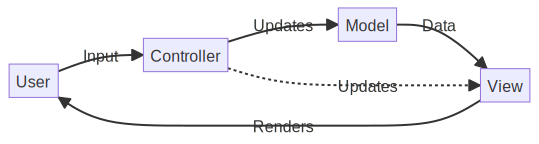
\includegraphics[width=\textwidth]{../images/mvc-classic.png}
	\caption{Classic MVC model when Users with controllers not screens}
	\label{fig:mvc-classic}
\end{figure}

\subsection{MVC dalam Kerangka Web dan Aplikasi Desktop Modern}

Banyak kerangka kerja web modern, seperti Laravel, Django, dan Spring, serta aplikasi desktop seperti JavaFX, menggunakan pendekatan MVC yang sedikit berbeda. Dalam implementasi ini:

\begin{itemize}
	\item Controller sering kali memiliki peran lebih besar, menangani logika bisnis dan interaksi dengan Model.
	\item View tidak hanya menampilkan data tetapi juga dapat berisi kode pemrograman untuk rendering dinamis.
	\item Model sering kali terintegrasi dengan ORM (\textit{Object-Relational Mapping}) untuk mempermudah akses ke basis data.
\end{itemize}

Diagram berikut menggambarkan perbedaan antara MVC klasik dan yang digunakan dalam kerangka kerja web dan aplikasi desktop modern:

\begin{figure}[h]
	\centering
	\includegraphics[width=\textwidth]{../images/mvc-modern.png}
	\caption{MVC in modern desktop/web frameworks.}
	\label{fig:mvc-modern}
\end{figure}

Pendekatan dalam kerangka kerja modern memungkinkan pemisahan lebih baik antara logika bisnis dan antarmuka pengguna, sekaligus mengintegrasikan teknologi seperti API REST dan AJAX untuk interaksi yang lebih dinamis.


\section{Model-View-Presenter (MVP)}

Model-View-Presenter (MVP) adalah pola desain yang mirip dengan MVC namun memiliki perbedaan signifikan dalam cara interaksi antara komponen-komponen tersebut. MVP lebih banyak digunakan dalam aplikasi desktop atau aplikasi yang membutuhkan pengendalian lebih besar terhadap tampilan dan interaksi pengguna. Dalam implementasi MVP:

\begin{itemize}
	\item \textbf{Model} bertanggung jawab untuk menangani logika bisnis dan data. Ini berinteraksi dengan basis data dan menyediakan data yang diperlukan oleh Presenter.
	\item \textbf{View} hanya bertugas untuk menampilkan antarmuka pengguna dan tidak mengandung logika bisnis. View akan menerima input dari pengguna dan meneruskannya ke Presenter. View bersifat pasif, artinya tidak mengelola pengolahan data atau logika bisnis.
	\item \textbf{Presenter} bertindak sebagai penghubung antara Model dan View. Presenter menerima input dari View, memprosesnya (dengan berinteraksi dengan Model), dan kemudian memperbarui View dengan data yang diperlukan.
\end{itemize}

Perbedaan utama antara \textbf{MVP} dan \textbf{MVC Klasik} terletak pada bagaimana komponen-komponen tersebut berinteraksi:
\begin{itemize}
	\item Dalam \textbf{MVP}, \textbf{Presenter} memiliki peran yang lebih besar. Semua logika bisnis dan pengolahan data dikelola oleh Presenter. View bertanggung jawab hanya untuk menampilkan data dan menerima input dari pengguna, tetapi tidak menangani pengolahan atau logika bisnis. Presenter mengelola interaksi antara Model dan View.
	\item Dalam \textbf{MVC Klasik}, \textbf{Controller} bertanggung jawab untuk menangani logika bisnis dan interaksi antara Model dan View. View hanya menampilkan data dan berinteraksi langsung dengan Controller. Dengan kata lain, Controller mempengaruhi tampilan berdasarkan aksi pengguna dengan mengubah Model, sedangkan View hanya berfungsi untuk menampilkan antarmuka pengguna.
	\item Dalam \textbf{MVP}, komunikasi antara View dan Presenter adalah dua arah, sementara dalam \textbf{MVC Klasik}, komunikasi lebih cenderung satu arah dari Controller ke View atau Model ke View.
\end{itemize}

Diagram berikut menggambarkan arsitektur MVP dan perbedaan utamanya dengan MVC Klasik:

\begin{figure}[h]
	\centering
	\includegraphics[width=\textwidth]{../images/mvp.png}
	\caption{Model-View-Presenter Architecture.}
	\label{fig:mvp-architecture}
\end{figure}

Keuntungan utama dari MVP adalah pemisahan yang jelas antara logika bisnis dan antarmuka pengguna, serta kemudahan pengujian unit karena Presenter dapat diuji secara terpisah tanpa bergantung pada View.

\section{Model-View-ViewModel (MVVM)}

Model-View-ViewModel (MVVM) adalah pola desain yang lebih banyak digunakan dalam aplikasi desktop dan aplikasi berbasis WPF (Windows Presentation Foundation) atau platform lain yang mendukung binding data dua arah. MVVM memisahkan logika presentasi dari antarmuka pengguna dengan cara yang sangat terstruktur. Dalam implementasi MVVM:

\begin{itemize}
	\item \textbf{Model} bertanggung jawab untuk menangani logika bisnis dan data. Model ini berinteraksi dengan basis data atau layanan lain untuk menyediakan data yang diperlukan oleh ViewModel.
	\item \textbf{View} bertanggung jawab untuk menampilkan antarmuka pengguna dan menerima input dari pengguna. View hanya berfokus pada rendering dan tidak mengelola logika atau data.
	\item \textbf{ViewModel} adalah penghubung antara View dan Model. ViewModel menangani logika presentasi, memanipulasi data yang diterima dari Model, dan menyediakan data tersebut dalam bentuk yang dapat digunakan oleh View. Dalam MVVM, ViewModel berinteraksi dengan View menggunakan binding data dua arah, yang memungkinkan pembaruan secara otomatis antara View dan ViewModel.
\end{itemize}

Perbedaan utama antara \textbf{MVVM} dan \textbf{MVP} terletak pada peran **ViewModel** dalam MVVM:
\begin{itemize}
	\item Dalam \textbf{MVVM}, \textbf{ViewModel} berfungsi untuk mempersiapkan data dari Model agar dapat digunakan oleh View. ViewModel mengelola logika presentasi dan menyediakan data dalam format yang dapat langsung dipakai oleh View.
	\item Dalam \textbf{MVP}, \textbf{Presenter} bertanggung jawab untuk memproses input dari View dan mengatur interaksi dengan Model, sementara View hanya menampilkan data dan tidak terlibat dalam pengolahan data atau logika.
	\item Dalam \textbf{MVVM}, komunikasi antara View dan ViewModel menggunakan binding data dua arah, memungkinkan pembaruan otomatis antara keduanya. Sebaliknya, dalam \textbf{MVP}, komunikasi antara View dan Presenter adalah satu arah, dimana Presenter memperbarui View dengan data yang diproses.
\end{itemize}

Diagram berikut menggambarkan arsitektur MVVM dan perbedaan utamanya dengan MVP:

\begin{figure}[h]
	\centering
	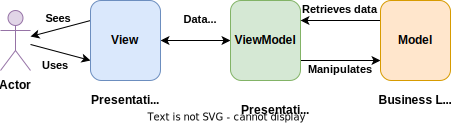
\includegraphics[width=\textwidth]{../images/mvvm.png}
	\caption{Model-View-ViewModel Architecture.}
	\label{fig:mvvm-architecture}
\end{figure}

Keuntungan utama dari MVVM adalah kemampuan untuk memisahkan logika presentasi dari antarmuka pengguna dengan menggunakan binding data dua arah, sehingga membuat pengujian dan pemeliharaan aplikasi lebih mudah. Selain itu, karena ViewModel menangani logika presentasi, View menjadi lebih sederhana dan lebih fokus pada rendering.


\section{Model-View-Intent (MVI)}

Model-View-Intent (MVI) adalah pola desain yang sering digunakan dalam aplikasi modern, terutama dalam pengembangan aplikasi Android. MVI bertujuan untuk menyederhanakan alur data dengan memberikan pendekatan yang lebih deklaratif dan reaktif. Dalam MVI, setiap komponen memiliki peran yang jelas dalam memanipulasi dan mengelola data aplikasi.

Dalam implementasi MVI:

\begin{itemize}
	\item \textbf{Model} berfungsi untuk menangani logika bisnis dan data aplikasi. Model ini menyediakan status atau keadaan aplikasi yang dapat digunakan oleh View. Model mengelola dan menyimpan data yang digunakan oleh aplikasi.
	\item \textbf{View} bertanggung jawab untuk menampilkan antarmuka pengguna dan menerima input dari pengguna. View akan mengirimkan intent ke Presenter atau ViewModel yang akan diproses lebih lanjut. View bersifat reaktif, menerima pembaruan dari Model melalui observasi data.
	\item \textbf{Intent} adalah tindakan atau niat yang dilakukan oleh pengguna yang kemudian diteruskan ke Presenter atau ViewModel untuk diproses. Intent menggambarkan apa yang ingin dilakukan oleh pengguna (misalnya, tombol ditekan atau elemen lainnya dipilih). Intent digunakan untuk memicu perubahan status pada Model atau memulai proses lain yang relevan.
\end{itemize}

Perbedaan utama antara \textbf{MVI} dan \textbf{MVP} terletak pada cara interaksi dan komunikasi antar komponen:
\begin{itemize}
	\item Dalam \textbf{MVI}, \textbf{Intent} menggantikan peran input pengguna yang secara langsung diteruskan ke ViewModel atau Presenter. Intent memfokuskan pada pengelolaan status aplikasi secara reaktif.
	\item Dalam \textbf{MVP}, \textbf{Presenter} bertanggung jawab untuk menangani logika presentasi dan memproses input dari View untuk memperbarui Model.
	\item Dalam \textbf{MVI}, komunikasi adalah satu arah dari Intent ke ViewModel atau Presenter, yang kemudian memodifikasi status Model dan mengirimkan pembaruan kembali ke View.
\end{itemize}

Diagram berikut menggambarkan arsitektur MVI dan perbedaannya dengan pola desain lain seperti MVP:

\begin{figure}[h]
	\centering
	\includegraphics[width=\textwidth]{../images/mvi.png}
	\caption{Model-View-Intent Architecture.}
	\label{fig:mvi-architecture}
\end{figure}

Keuntungan utama dari MVI adalah pengelolaan status aplikasi yang lebih sederhana dan kemampuan untuk menangani alur data yang lebih reaktif. MVI juga memudahkan pemeliharaan kode dengan mengurangi kebingungan terkait interaksi antara View dan Model, serta memperkenalkan pendekatan yang lebih terstruktur untuk menangani state.


\section{Contoh:}

Bagian ini menyajikan contoh implementasi arsitektur perangkat lunak menggunakan bahasa pemrograman Java dengan pustaka Java Swing. Implementasi ini menggunakan dua buah komponen \texttt{JSpinner}, di mana perubahan nilai pada \texttt{JSpinner} asal akan mempengaruhi nilai pada \texttt{JSpinner} tujuan. Perubahan nilai tidak terjadi secara langsung, melainkan diproses terlebih dahulu sesuai dengan arsitektur yang digunakan.

Setiap arsitektur memiliki pendekatan yang berbeda dalam menangani perubahan nilai pada \texttt{JSpinner}. Dalam Model-View-Controller (MVC), perubahan nilai dikelola oleh controller, yang bertanggung jawab sebagai perantara antara tampilan dan model. Dalam Model-View-Presenter (MVP), presenter mengambil alih peran perantara dengan mengelola logika pembaruan nilai. Model-View-ViewModel (MVVM) menggunakan mekanisme binding untuk menyinkronkan perubahan nilai antara tampilan dan model secara otomatis. Sementara itu, Model-View-Intent (MVI) menggunakan intent sebagai mekanisme untuk mengirimkan perubahan dari tampilan ke model.

Setiap arsitektur yang disajikan dalam bagian ini akan disertai dengan diagram urutan (sequence diagram) untuk menjelaskan bagaimana interaksi antara komponen terjadi dalam menangani perubahan nilai pada \texttt{JSpinner}. Diagram tersebut akan memberikan gambaran bagaimana data mengalir dari tampilan ke model serta bagaimana nilai diperbarui dalam sistem.


\subsection{Model-View-Controller (MVC)}
\begin{figure}[h]
	\centering
	\includegraphics[width=\textwidth]{../images/out/mvc-sequence}
	\caption{Model-View-Sequence Architecture.}
	\label{fig:mvc-sequence}
\end{figure}

Diagram urutan ini menggambarkan interaksi antara pengguna, tampilan (view), controller, dan model dalam arsitektur Model-View-Controller (MVC). Diagram ini menjelaskan bagaimana perubahan dalam antarmuka pengguna diproses melalui controller sebelum diperbarui di model dan tampilan.

Ketika \textbf{Pengguna} mengubah nilai pada spinner di antarmuka grafis, aksi ini ditangkap oleh \textbf{View}. Selanjutnya, view meneruskan perubahan ini ke \textbf{Controller} melalui metode \texttt{handleChange()} dengan parameter nama model, nama spinner, dan nilai baru.

Controller bertindak sebagai perantara antara view dan model dengan langkah-langkah sebagai berikut:

\begin{itemize}
	\item Controller menerima permintaan perubahan dari view dan meneruskannya ke \textbf{Model} dengan memanggil metode \texttt{setValue()} untuk memperbarui data yang sesuai.
	\item Model kemudian memperbarui data internalnya dengan nilai baru yang diberikan oleh controller.
	\item Setelah perubahan data selesai, model memperbarui \textbf{View} agar tampilan merefleksikan perubahan nilai yang telah terjadi.
\end{itemize}

Dalam arsitektur MVC, \textbf{Controller} bertanggung jawab untuk menangani interaksi pengguna dan meneruskan data ke model. Model menyimpan dan mengelola logika bisnis serta perubahan data, sementara view hanya menampilkan hasil tanpa menangani logika bisnis secara langsung.

Pendekatan ini memisahkan logika aplikasi dari antarmuka pengguna, membuat kode lebih mudah dipelihara dan diperluas. Selain itu, arsitektur MVC memungkinkan modularitas yang lebih besar, di mana model dan view dapat diperbarui atau diganti tanpa mengubah komponen lainnya.

Secara keseluruhan, diagram urutan ini menunjukkan bagaimana Model-View-Controller (MVC) mengelola aliran data dengan pendekatan yang lebih terstruktur, memastikan keterpisahan yang jelas antara presentasi, logika bisnis, dan data.


\subsection{Model-View-Presenter (MVP)}
\begin{figure}[h]
	\centering
	\includegraphics[width=\textwidth]{../images/out/mvp-sequence}
	\caption{Model-View-Presenter Sequence Architecture.}
	\label{fig:mvp-sequence}
\end{figure}

Diagram urutan ini menggambarkan interaksi antara pengguna, tampilan (view), presenter, dan model dalam arsitektur Model-View-Presenter (MVP). Diagram ini menjelaskan bagaimana perubahan dalam antarmuka pengguna diproses dan dikendalikan oleh presenter sebelum diperbarui di model dan tampilan.

Ketika \textbf{Pengguna} mengubah nilai pada spinner di antarmuka grafis, aksi ini ditangkap oleh \textbf{View}. Selanjutnya, view meneruskan perubahan ini ke \textbf{Presenter} melalui metode \texttt{stateChanged()}.

Presenter bertindak sebagai perantara antara view dan model dengan langkah-langkah sebagai berikut:

\begin{itemize}
	\item Presenter mengirimkan nilai baru ke \textbf{Model} dengan memanggil metode \texttt{setValue()} untuk memperbarui data yang sesuai.
	\item Setelah nilai diperbarui, presenter mengambil kembali nilai terbaru dari model dengan memanggil metode \texttt{getValue()}.
	\item Model mengembalikan nilai yang diperbarui ke presenter.
	\item Presenter kemudian memperbarui tampilan dengan mengirimkan nilai terbaru ke \textbf{View}, memastikan bahwa antarmuka pengguna mencerminkan perubahan yang telah terjadi.
\end{itemize}

Dalam arsitektur MVP, \textbf{Presenter} bertanggung jawab penuh untuk menangani logika aplikasi dan komunikasi antara view serta model. Hal ini memastikan bahwa view hanya menangani rendering antarmuka pengguna tanpa menyimpan atau mengelola data bisnis.

Pendekatan ini meningkatkan pemisahan tanggung jawab (Separation of Concerns), membuat kode lebih mudah diuji karena presenter dapat diuji secara terpisah dari view. Selain itu, arsitektur MVP memungkinkan fleksibilitas yang lebih besar dalam mengganti tampilan tanpa mengubah logika aplikasi di presenter.

Secara keseluruhan, diagram urutan ini menunjukkan bagaimana Model-View-Presenter (MVP) mengelola aliran data dan pembaruan tampilan dengan pendekatan yang lebih terstruktur dan terorganisir.


\subsection{Model-View-ViewModel (MVVM)}
\begin{figure}[h]
	\centering
	\includegraphics[width=\textwidth]{../images/out/mvvm-sequence}
	\caption{Model-View-ViewModel Sequence Architecture.}
	\label{fig:mvvm-sequence}
\end{figure}

Diagram urutan ini menggambarkan interaksi antara pengguna, tampilan (view), binder, properti ViewModel, ViewModel, dan model dalam arsitektur Model-View-ViewModel (MVVM). Diagram ini menjelaskan bagaimana perubahan dalam antarmuka pengguna diproses dan disinkronkan dengan model menggunakan mekanisme binding.

Ketika \textbf{Pengguna} mengubah nilai pada spinner di antarmuka grafis, aksi ini ditangkap oleh \textbf{View}. Selanjutnya, view mengirimkan perubahan ini ke \textbf{Binder} melalui metode \texttt{stateChanged()}. Binder bertugas untuk menjembatani komunikasi antara ViewModelProperty dan ViewModel.

Binder kemudian melakukan langkah-langkah berikut untuk memastikan data tetap sinkron antara view dan model:

\begin{itemize}
	\item Binder mengubah nilai pada \textbf{ViewModelProperty} dengan memanggil metode \texttt{setValue()}.
	\item Setelah nilai diperbarui, binder memberi tahu \textbf{ViewModel} tentang perubahan ini melalui metode \texttt{onPropertyChanged()}.
	\item ViewModel kemudian memperbarui \textbf{Model} dengan memanggil metode \texttt{setValue()} untuk menyimpan nilai baru.
	\item Setelah itu, ViewModel mengambil nilai terbaru dari Model menggunakan metode \texttt{getValue()}.
	\item Model mengembalikan nilai yang diperbarui ke ViewModel.
	\item ViewModel memperbarui nilai dalam \textbf{ViewModelProperty} dengan nilai yang baru.
	\item ViewModelProperty memberi tahu \textbf{Binder} bahwa perubahan telah terjadi melalui metode \texttt{onPropertyChanged()}.
	\item Terakhir, binder memperbarui tampilan (View) agar komponen yang terkait mencerminkan nilai yang telah diperbarui.
\end{itemize}

Arsitektur MVVM memastikan bahwa tampilan hanya berfungsi sebagai antarmuka pengguna tanpa menangani logika bisnis secara langsung. Binder bertugas sebagai penghubung antara View dan ViewModel untuk memastikan sinkronisasi data berjalan otomatis. 

Dengan menggunakan properti ViewModel dan mekanisme binding, arsitektur ini memungkinkan pemisahan tanggung jawab yang lebih jelas antara lapisan presentasi dan data. Pendekatan ini meningkatkan pemeliharaan kode dan memungkinkan pengujian yang lebih mudah karena ViewModel dapat diuji secara terpisah dari tampilan.

Secara keseluruhan, diagram urutan ini menunjukkan bagaimana Model-View-ViewModel (MVVM) mengelola perubahan status dengan cara yang terorganisir dan efisien, memastikan bahwa data selalu tersinkronisasi antara model dan tampilan.


\subsection{Model-View-Intent (MVI)}
\begin{figure}[h]
	\centering
	\includegraphics[width=\textwidth]{../images/out/mvi-sequence}
	\caption{Model-View-Intent Sequence Architecture.}
	\label{fig:mvi-sequence}
\end{figure}

Diagram urutan ini menggambarkan interaksi antara pengguna, tampilan (view), model, dan intent dalam arsitektur Model-View-Intent (MVI). Diagram ini menjelaskan bagaimana perubahan dalam antarmuka pengguna diproses dan diteruskan melalui sistem.

Ketika \textbf{Pengguna} mengubah nilai pada spinner di antarmuka grafis, aksi ini ditangkap oleh \textbf{View}. Selanjutnya, view membuat sebuah instance dari \texttt{UpdateValueIntent}, yang berisi nilai baru yang akan diperbarui serta komponen target yang akan menerima nilai tersebut. Intent ini berfungsi sebagai pesan terstruktur yang memberikan instruksi kepada model mengenai perubahan yang perlu dilakukan.

Setelah intent dibuat, view memanggil metode \texttt{handleIntent()} pada \textbf{Model}, dengan mengirimkan \texttt{UpdateValueIntent} sebagai parameter. Model kemudian memproses intent berdasarkan tipenya dengan mekanisme percabangan sebagai berikut:

\begin{itemize}
	\item \textbf{Jika intent adalah \texttt{UpdateValueIntent}}, model akan memperbarui nilai yang sesuai dengan memanggil metode \texttt{setValue()}. Selanjutnya, nilai yang diperbarui diambil kembali menggunakan metode \texttt{getValue()}. Setelah itu, model akan memperbarui tampilan dengan memanggil metode \texttt{updateViewState()} dan mengirimkan nilai yang telah diperbarui. Hal ini memastikan bahwa antarmuka pengguna selalu merefleksikan perubahan yang terjadi di dalam model.
	\item \textbf{Jika intent adalah tipe lain (\texttt{OtherIntent})}, model akan menjalankan aksi berbeda, yang mungkin melibatkan perhitungan tambahan atau perubahan status lainnya. Setelah operasi yang sesuai dijalankan, model akan memperbarui tampilan agar perubahan yang terjadi dapat terlihat pada antarmuka pengguna.
\end{itemize}

Arsitektur ini memastikan pemisahan tanggung jawab yang jelas dengan mendelegasikan pembaruan UI ke view, sementara model bertanggung jawab atas logika bisnis dan pengelolaan data. Pola ini meningkatkan kemudahan pemeliharaan serta pengujian dengan mengurangi keterkaitan langsung antara antarmuka pengguna dan logika aplikasi.

Dengan menggunakan intent, sistem menyediakan mekanisme terstruktur untuk mengelola perubahan status antara view dan model. Pendekatan ini memungkinkan manajemen status yang lebih baik dan memastikan bahwa semua perubahan diproses secara eksplisit melalui model, bukan langsung dimodifikasi di dalam view.

Secara keseluruhan, diagram urutan ini merepresentasikan implementasi arsitektur Model-View-Intent yang kuat, yang mendorong aliran data searah dan mengurangi ketergantungan antara komponen.

\chapter{Ports and Adapters Architecture}

\section{Pendahuluan}

Dalam pengembangan perangkat lunak, pemilihan arsitektur yang tepat menjadi salah satu faktor penentu keberhasilan sebuah aplikasi. Arsitektur yang baik memungkinkan aplikasi untuk tetap fleksibel, dapat diperluas, dan mudah dipelihara seiring perkembangan teknologi dan kebutuhan bisnis. Salah satu tantangan utama dalam pengembangan aplikasi adalah mengelola ketergantungan antara berbagai komponen, terutama antara logika bisnis dan teknologi eksternal seperti database, API, dan antarmuka pengguna.

Hexagonal Architecture, atau yang dikenal sebagai \textbf{Ports and Adapters Architecture}, adalah pendekatan yang dirancang untuk mengatasi tantangan ini. Dengan memisahkan logika bisnis inti dari teknologi eksternal, arsitektur ini memberikan fleksibilitas yang lebih besar dalam perubahan sistem, memungkinkan pengujian yang lebih mudah, serta meningkatkan modularitas aplikasi. Arsitektur ini pertama kali diperkenalkan oleh \textbf{Alistair Cockburn} pada tahun 2005 dan sejak saat itu telah menjadi salah satu pola yang banyak digunakan dalam pengembangan perangkat lunak modern.

Dokumen ini membahas konsep, prinsip, dan implementasi \textbf{Hexagonal Architecture} dalam bahasa pemrograman \textbf{Java}. Melalui pendekatan ini, pengembang dapat membangun aplikasi yang lebih terstruktur, terisolasi dari perubahan teknologi, dan lebih mudah diuji serta dipelihara.

\section{Latar Belakang}

Dalam pengembangan perangkat lunak, arsitektur aplikasi memiliki peran penting dalam menentukan bagaimana komponen-komponen di dalamnya berinteraksi. Arsitektur tradisional, seperti \textit{layered architecture} (n-tier architecture), sering kali menghasilkan ketergantungan yang kuat antara lapisan-lapisannya. Misalnya, perubahan dalam lapisan penyimpanan data dapat berdampak langsung pada lapisan logika bisnis dan presentasi, sehingga menyulitkan perawatan dan pengembangan lebih lanjut.

Untuk mengatasi masalah tersebut, berbagai pendekatan arsitektur perangkat lunak yang lebih fleksibel dan modular telah dikembangkan. Salah satu pendekatan yang muncul adalah \textbf{Hexagonal Architecture}, yang juga dikenal sebagai \textit{Ports and Adapters Architecture}. Konsep ini pertama kali diperkenalkan oleh \textbf{Alistair Cockburn} pada tahun 2005 dengan tujuan utama memisahkan logika bisnis inti dari teknologi eksternal, seperti database, API, dan antarmuka pengguna. Dengan pendekatan ini, perubahan pada salah satu komponen tidak akan berdampak langsung pada komponen lainnya.

\subsection{Sejarah Hexagonal Architecture}

Hexagonal Architecture lahir dari kebutuhan untuk menciptakan perangkat lunak yang lebih \textit{modular}, mudah diuji, dan fleksibel terhadap perubahan teknologi. Pada awal tahun 2000-an, banyak aplikasi monolitik memiliki ketergantungan yang kuat terhadap framework dan teknologi spesifik, yang menyebabkan kesulitan dalam melakukan migrasi atau perubahan arsitektur.

Alistair Cockburn memperkenalkan konsep ini dengan gagasan utama bahwa logika bisnis inti harus diisolasi dari dunia luar melalui \textbf{ports} (antarmuka komunikasi) dan \textbf{adapters} (implementasi yang memungkinkan komunikasi dengan teknologi eksternal). Dengan struktur ini, suatu aplikasi dapat dengan mudah diuji menggunakan \textit{mock} atau \textit{stub} tanpa bergantung pada teknologi seperti database atau layanan eksternal lainnya.

Konsep ini kemudian mendapat lebih banyak perhatian seiring berkembangnya praktik \textbf{Clean Architecture} yang diperkenalkan oleh \textbf{Robert C. Martin} (Uncle Bob) serta pendekatan berbasis \textbf{Domain-Driven Design (DDD)} yang dipopulerkan oleh \textbf{Eric Evans}. Hingga saat ini, Hexagonal Architecture banyak diadopsi dalam pengembangan aplikasi modern, terutama pada sistem yang membutuhkan fleksibilitas tinggi dalam mengintegrasikan berbagai teknologi.

\subsection{Motivasi Penggunaan Hexagonal Architecture}

Beberapa alasan utama mengapa Hexagonal Architecture semakin banyak digunakan dalam pengembangan perangkat lunak adalah sebagai berikut:

\begin{itemize}
	\item \textbf{Memisahkan logika bisnis dari ketergantungan teknologi} \\
	Dengan adanya \textit{ports and adapters}, perubahan pada teknologi penyimpanan data, framework, atau sistem eksternal lainnya tidak berdampak langsung pada domain bisnis.
	
	\item \textbf{Memudahkan pengujian unit dan integrasi} \\
	Karena tidak ada ketergantungan langsung dengan teknologi eksternal, pengujian dapat dilakukan secara independen tanpa memerlukan koneksi ke database atau layanan eksternal.
	
	\item \textbf{Fleksibilitas dalam penggantian teknologi} \\
	Dengan pendekatan ini, tim pengembang dapat mengganti database, sistem pesan, atau antarmuka pengguna tanpa harus mengubah logika bisnis yang sudah ada.
	
	\item \textbf{Struktur yang lebih modular dan mudah dikembangkan} \\
	Arsitektur ini memudahkan pengembang dalam menambahkan fitur baru atau mengganti bagian dari sistem tanpa merusak keseluruhan sistem.
\end{itemize}

Dengan semua manfaat tersebut, Hexagonal Architecture menjadi solusi yang kuat untuk membangun perangkat lunak yang \textbf{fleksibel}, \textbf{dapat dipelihara}, dan \textbf{mudah diuji}.


\section{Definisi, Prinsip, dan Struktur Hexagonal Architecture}

Hexagonal Architecture, yang juga dikenal sebagai \textit{Ports and Adapters Architecture}, adalah pola arsitektur perangkat lunak yang bertujuan untuk memisahkan logika bisnis inti dari teknologi eksternal seperti database, API, dan antarmuka pengguna. Konsep ini memungkinkan fleksibilitas dalam mengubah teknologi yang digunakan tanpa perlu mengubah logika inti aplikasi.

Pendekatan ini didasarkan pada ide bahwa sebuah sistem harus memiliki antarmuka yang jelas dalam berkomunikasi dengan dunia luar. Hal ini dicapai melalui penggunaan \textbf{ports} (antarmuka komunikasi) dan \textbf{adapters} (implementasi yang memungkinkan interaksi dengan teknologi eksternal). Dengan demikian, komponen dalam aplikasi tidak memiliki ketergantungan langsung terhadap teknologi spesifik.

\subsection{Prinsip Hexagonal Architecture}

Hexagonal Architecture memiliki beberapa prinsip utama yang menjadi dasar penerapannya:

\begin{itemize}
	\item \textbf{Pemisahan Logika Bisnis dan Teknologi Eksternal} \\
	Logika bisnis diletakkan di bagian inti (\textit{domain}) aplikasi, sementara detail teknis seperti database, layanan eksternal, dan antarmuka pengguna hanya berinteraksi melalui \textit{ports and adapters}.
	
	\item \textbf{Interaksi Melalui Ports dan Adapters} \\
	Semua interaksi antara domain bisnis dan dunia luar dilakukan melalui \textit{ports} (interface yang mendefinisikan kontrak komunikasi) dan \textit{adapters} (implementasi dari ports yang berkomunikasi dengan teknologi tertentu).
	
	\item \textbf{Dukungan terhadap Pengujian yang Lebih Mudah} \\
	Dengan struktur ini, unit bisnis dapat diuji secara independen tanpa harus bergantung pada database atau sistem eksternal lainnya. Hal ini memungkinkan penggunaan \textit{mock} atau \textit{stub} dalam pengujian.
	
	\item \textbf{Fleksibilitas dalam Perubahan Teknologi} \\
	Karena teknologi eksternal hanya dihubungkan melalui adapters, mengganti database, framework, atau layanan eksternal lainnya dapat dilakukan tanpa mengubah logika inti aplikasi.
\end{itemize}

\subsection{Struktur Hexagonal Architecture}

Gambar \ref{fig:hexagonal_architecture} menunjukkan bagaimana komponen-komponen dalam Hexagonal Architecture saling berinteraksi:

\begin{figure}[h]
	\centering
	\includegraphics[width=.8\textwidth]{../images/hexagonal_architecture.png}
	\caption{Hexagonal Architecture}
	\label{fig:hexagonal_architecture}
\end{figure}

Hexagonal Architecture membagi sistem menjadi tiga bagian utama:

\begin{enumerate}
	\item \textbf{Domain} \\
	Domain merupakan inti dari aplikasi yang berisi logika bisnis utama. Bagian ini harus bebas dari ketergantungan terhadap teknologi eksternal agar tetap bersifat murni (\textit{pure business logic}).
	
	\item \textbf{Ports} \\
	Ports adalah antarmuka yang menghubungkan domain dengan dunia luar. Ports mendefinisikan kontrak komunikasi yang digunakan oleh adapters untuk berinteraksi dengan domain.
	
	\item \textbf{Adapters} \\
	Adapters adalah implementasi dari ports yang memungkinkan interaksi dengan teknologi eksternal, seperti database, sistem pesan, atau antarmuka pengguna. Adapters bertanggung jawab untuk menerjemahkan data dari format eksternal ke format yang dapat dipahami oleh domain.
\end{enumerate}




\section{Kelebihan Hexagonal Architecture}

Hexagonal Architecture memiliki berbagai keunggulan dalam pengembangan perangkat lunak, terutama dalam hal modularitas, kemudahan pengujian, dan fleksibilitas terhadap perubahan teknologi. Berikut adalah beberapa kelebihan utama dari pendekatan ini:

\begin{enumerate}
	\item \textbf{Pemisahan Logika Bisnis dan Teknologi Eksternal} \\
	Logika bisnis ditempatkan di dalam \textit{domain}, sementara interaksi dengan teknologi eksternal seperti database, API, atau sistem pesan hanya dilakukan melalui \textit{ports} dan \textit{adapters}. Hal ini memastikan bahwa perubahan pada teknologi eksternal tidak berdampak langsung pada logika bisnis utama.
	
	\item \textbf{Memudahkan Pengujian Unit dan Integrasi} \\
	Karena domain tidak memiliki ketergantungan langsung terhadap teknologi eksternal, pengujian dapat dilakukan secara mandiri menggunakan \textit{mock} atau \textit{stub}. Dengan demikian, pengembang dapat menguji logika bisnis tanpa perlu bergantung pada infrastruktur seperti database atau layanan eksternal lainnya, sehingga meningkatkan kecepatan dan efektivitas pengujian.
	
	\item \textbf{Fleksibilitas dalam Penggantian Teknologi} \\
	Dengan adanya lapisan \textit{adapters}, teknologi yang digunakan di sisi luar domain dapat diganti tanpa mengubah kode dalam logika bisnis. Misalnya, jika sebuah aplikasi awalnya menggunakan MySQL sebagai penyimpanan data dan kemudian ingin beralih ke PostgreSQL atau MongoDB, perubahan tersebut dapat dilakukan dengan hanya mengganti implementasi adapter tanpa perlu mengubah domain atau layanan bisnis yang sudah ada.
	
	\item \textbf{Struktur yang Modular dan Mudah Dikembangkan} \\
	Dengan membagi aplikasi menjadi domain, ports, dan adapters, sistem menjadi lebih terorganisir dan mudah diperluas. Setiap komponen dapat dikembangkan secara independen, memungkinkan tim pengembang untuk bekerja secara paralel tanpa mengganggu bagian lain dari aplikasi.
	
	\item \textbf{Mendukung Prinsip Pemrograman yang Baik} \\
	Hexagonal Architecture mengikuti prinsip-prinsip pemrograman yang baik, seperti \textit{Separation of Concerns} (SoC) dan \textit{Dependency Inversion Principle} (DIP) dari SOLID. Dengan mengikuti prinsip-prinsip ini, kode menjadi lebih bersih, lebih terstruktur, dan lebih mudah dipahami serta dipelihara.
\end{enumerate}

Dengan semua keunggulan ini, Hexagonal Architecture menjadi pilihan yang ideal bagi pengembangan sistem yang membutuhkan fleksibilitas, skalabilitas, dan kemudahan pemeliharaan dalam jangka panjang.

\section{Kekurangan Hexagonal Architecture}

Meskipun Hexagonal Architecture memiliki banyak keunggulan, pendekatan ini juga memiliki beberapa kekurangan yang perlu dipertimbangkan sebelum diterapkan. Berikut adalah beberapa tantangan utama yang dapat dihadapi:

\begin{enumerate}
	\item \textbf{Kompleksitas Tambahan dalam Desain} \\
	Hexagonal Architecture memperkenalkan lapisan tambahan seperti \textit{ports} dan \textit{adapters}, yang meningkatkan kompleksitas desain sistem. Pengembang harus memahami cara menerapkan pola ini dengan benar agar manfaatnya dapat dimaksimalkan tanpa menambah beban yang tidak perlu.
	
	\item \textbf{Membutuhkan Lebih Banyak Kode} \\
	Dengan adanya pemisahan antara domain, ports, dan adapters, jumlah kode yang harus ditulis menjadi lebih banyak dibandingkan dengan arsitektur tradisional. Hal ini dapat memperpanjang waktu pengembangan dan meningkatkan beban pemeliharaan.
	
	\item \textbf{Kurva Belajar yang Lebih Curam} \\
	Pengembang yang belum familiar dengan konsep Hexagonal Architecture mungkin akan mengalami kesulitan dalam memahami cara kerja dan penerapannya. Dibutuhkan waktu untuk mempelajari dan mengadopsi pendekatan ini secara efektif.
	
	\item \textbf{Tidak Selalu Cocok untuk Aplikasi Sederhana} \\
	Untuk aplikasi kecil dengan kebutuhan bisnis yang sederhana, Hexagonal Architecture mungkin dianggap terlalu berlebihan. Struktur tambahan yang diperkenalkan dapat menjadi beban daripada keuntungan dalam proyek dengan kompleksitas rendah.
	
	\item \textbf{Meningkatkan Overhead dalam Komunikasi Antar Komponen} \\
	Karena setiap interaksi antara domain dan teknologi eksternal harus melalui ports dan adapters, ada potensi peningkatan overhead dalam komunikasi antar komponen dibandingkan dengan arsitektur yang lebih langsung.
\end{enumerate}

Meskipun memiliki beberapa kekurangan, Hexagonal Architecture tetap menjadi pilihan yang baik dalam pengembangan perangkat lunak yang membutuhkan fleksibilitas tinggi, kemudahan pengujian, dan skalabilitas jangka panjang.



\section{Contoh Implementasi dalam Java}

Untuk memahami bagaimana Hexagonal Architecture dapat diterapkan dalam pengembangan perangkat lunak menggunakan Java, berikut adalah contoh implementasi dengan studi kasus manajemen pengguna. Implementasi ini mencakup tiga komponen utama dalam Hexagonal Architecture: \textit{Domain}, \textit{Adapters}, dan layanan aplikasi.



\subsection{Definisi Domain}

Bagian \textbf{domain} merupakan inti dari sistem yang berisi logika bisnis utama. Domain harus dibuat sedemikian rupa sehingga tidak memiliki ketergantungan terhadap teknologi eksternal, seperti database, framework, atau sistem antarmuka pengguna. Dengan pendekatan ini, logika bisnis tetap bersifat murni (\textit{pure business logic}) dan dapat digunakan kembali tanpa bergantung pada detail implementasi teknis.

Domain dalam studi kasus ini adalah sistem manajemen akun pelanggan, yang mencakup validasi akun, pemrosesan saldo, dan transaksi pelanggan.

\begin{enumerate}
	\item \textbf{Entitas (\textit{Entity})} \\
	Entitas utama dalam domain ini adalah \texttt{CustomerAccount}, yang merepresentasikan akun pelanggan dengan fitur seperti ID unik, nama pelanggan, saldo akun, serta operasi bisnis seperti melakukan deposit dan penarikan saldo.
	
	\begin{lstlisting}[style=JavaStyle, caption=CustomerAccount Entity]
		public class CustomerAccount {
			private String id;
			private String name;
			private double balance;
			
			public CustomerAccount(String id, String name, double initialBalance) {
				if (initialBalance < 0) {
					throw new IllegalArgumentException("Saldo awal tidak boleh negatif.");
				}
				this.id = id;
				this.name = name;
				this.balance = initialBalance;
			}
			
			public String getId() { return id; }
			public String getName() { return name; }
			public double getBalance() { return balance; }
			
			public void deposit(double amount) {
				if (amount <= 0) {
					throw new IllegalArgumentException("Jumlah deposit harus lebih dari nol.");
				}
				this.balance += amount;
			}
			
			public void withdraw(double amount) {
				if (amount <= 0) {
					throw new IllegalArgumentException("Jumlah penarikan harus lebih dari nol.");
				}
				if (amount > this.balance) {
					throw new IllegalArgumentException("Saldo tidak mencukupi untuk penarikan.");
				}
				this.balance -= amount;
			}
		}
	\end{lstlisting}

	\begin{itemize}
		\item Kelas \texttt{CustomerAccount} merepresentasikan akun pelanggan dengan tiga atribut utama:
		\begin{itemize}
			\item \texttt{id}: ID unik pelanggan.
			\item \texttt{name}: Nama pelanggan.
			\item \texttt{balance}: Saldo akun pelanggan.
		\end{itemize}
		\item Konstruktor memastikan bahwa saldo awal tidak boleh negatif.
		\item Metode \texttt{deposit(double amount)} digunakan untuk menambahkan dana ke akun pelanggan dengan validasi jumlah yang harus lebih dari nol.
		\item Metode \texttt{withdraw(double amount)} memastikan bahwa pelanggan hanya dapat menarik saldo jika jumlahnya mencukupi dan lebih dari nol.
		\item Semua operasi dilakukan di dalam domain tanpa ketergantungan pada teknologi eksternal.
	\end{itemize}
	
	\item \textbf{Logika Bisnis ada di Domain} \\
	Dalam pendekatan Hexagonal Architecture, domain bertanggung jawab atas logika bisnis utama untuk menjaga isolasi dari teknologi eksternal. Beberapa alasan utama mengapa logika bisnis harus ditempatkan di domain adalah:
	\begin{itemize}
		\item Memastikan aturan bisnis tetap konsisten di seluruh aplikasi, terlepas dari teknologi yang digunakan.
		\item Memudahkan pengujian unit karena logika bisnis dapat diuji secara independen tanpa ketergantungan pada database atau antarmuka pengguna.
		\item Memungkinkan fleksibilitas dalam perubahan sistem tanpa harus mengubah keseluruhan arsitektur.
	\end{itemize}
\end{enumerate}

Dengan struktur ini, domain tetap fleksibel, modular, dan dapat digunakan kembali dalam berbagai skenario tanpa bergantung pada detail teknis tertentu.


\subsection{Definisi Port}

Dalam Hexagonal Architecture, \textbf{port} adalah antarmuka yang mendefinisikan bagaimana komponen domain berinteraksi dengan dunia luar, seperti layanan database, sistem eksternal, atau antarmuka pengguna. Port bertindak sebagai jembatan yang memungkinkan komunikasi antara domain dan teknologi eksternal tanpa menciptakan ketergantungan langsung terhadap implementasi spesifik.

\begin{enumerate}
	\item \textbf{Peran Port dalam Hexagonal Architecture} \\
	Port memiliki peran penting dalam menjaga modularitas dan fleksibilitas arsitektur, dengan beberapa fungsi utama:
	\begin{itemize}
		\item \textbf{Memisahkan logika bisnis dari teknologi eksternal} – Domain tidak perlu mengetahui detail teknis tentang bagaimana data disimpan atau bagaimana layanan lain bekerja.
		\item \textbf{Mendefinisikan kontrak komunikasi} – Port menentukan antarmuka yang harus diimplementasikan oleh teknologi eksternal, seperti database atau API.
		\item \textbf{Mempermudah pengujian unit} – Dengan menggunakan port, pengujian dapat dilakukan menggunakan \textit{mock} atau \textit{stub} tanpa bergantung pada implementasi nyata.
		\item \textbf{Memungkinkan perubahan teknologi tanpa mempengaruhi domain} – Jika teknologi penyimpanan data berubah (misalnya dari MySQL ke MongoDB), hanya adapter yang perlu diubah tanpa mempengaruhi logika bisnis.
	\end{itemize}
	
	\item \textbf{Jenis Port dalam Hexagonal Architecture} \\
	Dalam implementasi Hexagonal Architecture, terdapat dua jenis utama port:
	
	\begin{itemize}
		\item \textbf{Inbound Port (Driving Port)} \\
		Port ini digunakan untuk menerima permintaan dari luar dan meneruskannya ke domain. Contohnya adalah layanan API atau antarmuka pengguna yang memicu tindakan dalam domain.
		
		\item \textbf{Outbound Port (Driven Port)} \\
		Port ini digunakan oleh domain untuk berkomunikasi dengan dunia luar, seperti database atau layanan eksternal. Domain memanggil port ini, tetapi implementasinya ditentukan oleh adapter.
	\end{itemize}
	
	\item \textbf{Contoh Implementasi Port dalam Java} \\
	Dalam studi kasus manajemen akun pelanggan, kita mendefinisikan port untuk menghubungkan domain dengan lapisan penyimpanan data. Port ini memungkinkan domain menyimpan dan mengambil data pelanggan tanpa mengetahui detail teknis dari database.
	
	\begin{lstlisting}[style=JavaStyle, caption=CustomerAccountRepository Port]
		public interface CustomerAccountRepository {
			void save(CustomerAccount account);
			CustomerAccount findById(String id);
		}
	\end{lstlisting}
	
	\textbf{Penjelasan:}
	\begin{itemize}
		\item \texttt{CustomerAccountRepository} adalah port yang mendefinisikan kontrak untuk penyimpanan akun pelanggan.
		\item Metode \texttt{save(CustomerAccount account)} digunakan untuk menyimpan atau memperbarui akun pelanggan.
		\item Metode \texttt{findById(String id)} digunakan untuk mengambil akun pelanggan berdasarkan ID.
		\item Implementasi dari antarmuka ini akan dibuat dalam adapter yang berinteraksi dengan database.
	\end{itemize}
\end{enumerate}

Dengan pendekatan ini, domain tetap independen dari teknologi penyimpanan data. Jika di masa depan aplikasi ingin mengganti database dari SQL ke NoSQL, kita hanya perlu mengubah implementasi adapter tanpa menyentuh domain atau layanan bisnis yang sudah ada.


\subsection{Implementasi Adapter}

Dalam Hexagonal Architecture, \textbf{adapter} bertanggung jawab untuk menghubungkan domain dengan teknologi eksternal, seperti database. Adapter ini mengimplementasikan \textit{port} yang telah didefinisikan sebelumnya, yaitu \texttt{CustomerAccountRepository}, sehingga domain tetap bebas dari ketergantungan terhadap detail teknis penyimpanan data.

Pada implementasi ini, kita akan membuat dua adapter berbeda untuk mendukung dua jenis database: \textbf{MySQL} dan \textbf{PostgreSQL}. Keduanya akan mengimplementasikan port yang sama, sehingga domain tidak perlu mengetahui perbedaan di antara keduanya.

\begin{enumerate}
	\item \textbf{Implementasi Adapter untuk MySQL}
	
	Adapter ini menggunakan JDBC untuk berinteraksi dengan MySQL. Implementasi adapter MySQL dapat dilihat pada \ref{lst:mysql_adapter}. Kelas \texttt{MySQLCustomerAccountRepository} mengimplementasikan port \texttt{CustomerAccountRepository}, yang bertindak sebagai antarmuka antara domain bisnis dan database. Kelas ini menangani penyimpanan dan pengambilan data pelanggan dengan metode yang telah ditentukan dalam antarmuka.
	
	\begin{lstlisting}[style=JavaStyle, caption=MySQL Adapter Implementation, label=lst:mysql_adapter]
		public class MySQLCustomerAccountRepository implements CustomerAccountRepository {
			private Connection connection;
			
			// Konstruktor yang secara otomatis membuat koneksi ke database MySQL
			public MySQLCustomerAccountRepository() throws SQLException {
				this.connection = DriverManager.getConnection(
				"jdbc:mysql://localhost:3306/customer_db", "root", "secret"
				);
			}
			
			// Menyimpan akun pelanggan ke dalam database
			@Override
			public void save(CustomerAccount account) throws SQLException {
				String sql = "INSERT INTO customer_accounts (id, name, balance) VALUES (?, ?, ?)";
				PreparedStatement stmt = connection.prepareStatement(sql);
				stmt.setString(1, account.getId());
				stmt.setString(2, account.getName());
				stmt.setDouble(3, account.getBalance());
				stmt.executeUpdate();
			}
			
			// Mengambil akun pelanggan berdasarkan ID
			@Override
			public CustomerAccount findById(String id) throws SQLException {
				String sql = "SELECT * FROM customer_accounts WHERE id = ?";
				PreparedStatement stmt = connection.prepareStatement(sql);
				stmt.setString(1, id);
				ResultSet rs = stmt.executeQuery();
				
				if (rs.next()) {
					return new CustomerAccount(rs.getString("id"), rs.getString("name"), rs.getDouble("balance"));
				}
				return null;
			}
		}
	\end{lstlisting}
	
	Kelas ini memiliki beberapa fungsi utama:
	\begin{itemize}
		\item \textbf{Konstruktor:} \texttt{DriverManager.getConnection()} digunakan untuk membuka koneksi ke database MySQL menggunakan.
		\item \textbf{Metode \texttt{save()}:} Menggunakan prepared statement untuk menyimpan objek \texttt{CustomerAccount} ke dalam database guna mencegah SQL injection.
		\item \textbf{Metode \texttt{findById()}:} Mengeksekusi query untuk mencari akun pelanggan berdasarkan ID dan mengembalikan objek \texttt{CustomerAccount} jika ditemukan.
	\end{itemize}
	
	Pendekatan ini memungkinkan aplikasi berinteraksi dengan MySQL tanpa harus mengetahui detail implementasi spesifiknya. Dengan \textbf{Hexagonal Architecture}, perubahan sistem database tidak akan berdampak pada logika bisnis utama.
	

	\item \textbf{Implementasi Adapter untuk PostgreSQL}
	
	Adapter ini juga menggunakan JDBC dengan struktur yang mirip dengan MySQL. Implementasi adapter PostgreSQL dapat dilihat pada \ref{lst:postgres_adapter}. Kelas \texttt{PostgreSQLCus\-tomerAccountRepository} mengimplementasikan port \texttt{CustomerAccountReposito\-ry}, yang bertindak sebagai antarmuka antara domain bisnis dan database. Kelas ini menangani penyimpanan dan pengambilan data pelanggan dengan metode yang telah ditentukan dalam antarmuka.
	
	\begin{lstlisting}[style=JavaStyle, caption=PostgreSQL Adapter Implementation, label=lst:postgres_adapter]
		public class PostgreSQLCustomerAccountRepository implements CustomerAccountRepository {
			private Connection connection;
			
			// Konstruktor yang secara otomatis membuat koneksi ke database PostgreSQL
			public PostgreSQLCustomerAccountRepository() throws SQLException {
				this.connection = DriverManager.getConnection(
				"jdbc:postgresql://localhost:5432/customer_db", "postgres", "secret"
				);
			}
			
			// Menyimpan akun pelanggan ke dalam database
			@Override
			public void save(CustomerAccount account) throws SQLException {
				String sql = "INSERT INTO customer_accounts (id, name, balance) VALUES (?, ?, ?)";
				PreparedStatement stmt = connection.prepareStatement(sql);
				stmt.setString(1, account.getId());
				stmt.setString(2, account.getName());
				stmt.setDouble(3, account.getBalance());
				stmt.executeUpdate();
			}
			
			// Mengambil akun pelanggan berdasarkan ID
			@Override
			public CustomerAccount findById(String id) throws SQLException {
				String sql = "SELECT * FROM customer_accounts WHERE id = ?";
				PreparedStatement stmt = connection.prepareStatement(sql);
				stmt.setString(1, id);
				ResultSet rs = stmt.executeQuery();
				
				if (rs.next()) {
					return new CustomerAccount(rs.getString("id"), rs.getString("name"), rs.getDouble("balance"));
				}
				return null;
			}
		}
	\end{lstlisting}
	
	Kelas ini memiliki beberapa fungsi utama:
	\begin{itemize}
		\item \textbf{Konstruktor:} \texttt{DriverManager.getConnection()} digunakan untuk membuka koneksi ke database PostgreSQL.
		\item \textbf{Metode \texttt{save()}:} Menggunakan prepared statement untuk menyimpan objek \texttt{CustomerAccount} ke dalam database guna mencegah SQL injection.
		\item \textbf{Metode \texttt{findById()}:} Mengeksekusi query untuk mencari akun pelanggan berdasarkan ID dan mengembalikan objek \texttt{CustomerAccount} jika ditemukan.
	\end{itemize}
	
	Dengan menggunakan pendekatan yang seragam untuk kedua database, aplikasi tetap fleksibel dan dapat dengan mudah beralih antara MySQL dan PostgreSQL tanpa mengubah logika bisnis utama. Dengan \textbf{Hexagonal Architecture}, ketergantungan terhadap database tertentu dapat diminimalisir untuk meningkatkan skalabilitas dan fleksibilitas sistem.

	
	

	
\end{enumerate}

Pendekatan ini memastikan bahwa aplikasi dapat menggunakan MySQL atau PostgreSQL secara fleksibel tanpa mengubah logika bisnis utama. Dengan menggunakan \textbf{Hexagonal Architecture}, perubahan database tidak akan memengaruhi domain bisnis.



\subsection{Contoh Penggunaan}
Aplikasi konsol berikut menunjukkan cara menggunakan adapter MySQL atau PostgreSQL untuk menyimpan dan mengambil akun pelanggan. Implementasi utama dalam aplikasi konsol dapat dilihat pada \ref{lst:console_app}.

\begin{lstlisting}[style=JavaStyle, caption=Console Application Example, label=lst:console_app]
	public class Main {
		public static void main(String[] args) {
			try {
				// Menggunakan refleksi untuk menginstansiasi kelas repository secara dinamis
				CustomerAccountRepository repository = (CustomerAccountRepository)
				Class.forName("com.example.MySQLCustomerAccountRepository")
				.getDeclaredConstructor()
				.newInstance();
				
				// Membuat akun pelanggan baru
				CustomerAccount account = new CustomerAccount("C001", "Alice", 500.0);
				repository.save(account);
				
				// Mengambil akun pelanggan berdasarkan ID
				CustomerAccount retrieved = repository.findById("C001");
				
				// Menampilkan hasil pencarian akun pelanggan
				if (retrieved != null) {
					System.out.println("Customer: " + retrieved.getName() + 
					", Balance: " + retrieved.getBalance());
				} else {
					System.out.println("Customer not found.");
				}
			} catch (Exception e) {
				System.err.println("Terjadi kesalahan: " + e.getMessage());
				e.printStackTrace();
			}
		}
	}
\end{lstlisting}

Pendekatan ini menggunakan \textbf{Java Reflection} untuk menghindari ketergantungan langsung terhadap implementasi spesifik dari repository. Sistem dapat secara dinamis menentukan kelas repository yang akan digunakan dengan memanggil \texttt{Class.forName()} tanpa memerlukan pernyataan kondisional seperti \texttt{if-else}.

Kelebihan dari metode ini meliputi:
\begin{itemize}
	\item \textbf{Fleksibilitas}: Implementasi repository dapat diubah tanpa mengubah kode utama.
	\item \textbf{Dekoupling}: Mengurangi ketergantungan antara kelas utama dan implementasi spesifik repository.
	\item \textbf{Ekstensibilitas}: Memungkinkan penambahan repository lain di masa depan tanpa modifikasi kode utama.
\end{itemize}

Namun, pendekatan ini juga memiliki beberapa kelemahan, seperti:
\begin{itemize}
	\item \textbf{Kurangnya keamanan tipe}: Kesalahan nama kelas hanya dapat diketahui saat runtime, bukan saat kompilasi.
	\item \textbf{Kinerja}: Menggunakan refleksi memiliki sedikit overhead dibandingkan instansiasi langsung.
\end{itemize}

Pendekatan ini memastikan bahwa aplikasi dapat menggunakan MySQL atau PostgreSQL secara fleksibel tanpa mengubah logika bisnis utama. Dengan menggunakan \textbf{Hexagonal Architecture}, perubahan database tidak akan memengaruhi domain bisnis.


\section{Kesimpulan}

Hexagonal Architecture menawarkan pendekatan yang kuat dalam pengembangan perangkat lunak dengan memisahkan logika bisnis dari teknologi eksternal. Dengan menggunakan \textbf{ports} dan \textbf{adapters}, aplikasi menjadi lebih fleksibel, modular, dan dapat dengan mudah beradaptasi terhadap perubahan teknologi tanpa harus mengubah inti logika bisnis.

Beberapa manfaat utama dari Hexagonal Architecture meliputi:
\begin{itemize}
	\item \textbf{Pemisahan logika bisnis dan teknologi eksternal}, yang memungkinkan aplikasi tetap stabil meskipun ada perubahan dalam sistem eksternal.
	\item \textbf{Kemudahan pengujian}, karena logika bisnis dapat diuji secara mandiri tanpa bergantung pada database atau layanan eksternal.
	\item \textbf{Fleksibilitas dalam pergantian teknologi}, di mana database, sistem pesan, atau antarmuka pengguna dapat diubah tanpa harus mengubah domain aplikasi.
	\item \textbf{Struktur yang modular dan dapat dikembangkan}, memungkinkan pengembangan fitur baru tanpa mengganggu komponen lain dalam sistem.
\end{itemize}

Namun, Hexagonal Architecture juga memiliki beberapa tantangan, seperti meningkatnya kompleksitas desain dan kurva belajar yang lebih curam bagi pengembang yang belum familiar dengan konsep ini. Selain itu, penerapan arsitektur ini dapat memperbanyak jumlah kode dan meningkatkan overhead dalam komunikasi antar komponen.

Meskipun demikian, bagi aplikasi yang membutuhkan fleksibilitas tinggi, skalabilitas jangka panjang, dan pemeliharaan yang lebih mudah, Hexagonal Architecture menjadi pilihan yang sangat baik. Dengan penerapan yang tepat, arsitektur ini dapat membantu membangun sistem yang lebih tangguh, mudah diuji, dan berkelanjutan dalam menghadapi perubahan teknologi.




\chapter{Event-Driven Architecture}
\authors{Delvin, Gabrielle Sheila Sylvagno, Danica Recca Danendra}


\section{Event-Driven Architecture}
\subsection{Event-Driven Architecture}
\begin{figure}[h]
	\centering
	
\includegraphics[width=\textwidth]{diagram-EDA}
	\caption{Skema Diagram EDA}
	\label{fig:diagram-EDA}
\end{figure}
\textit{Event-driven architecture} (EDA) atau arsitektur berbasis peristiwa adalah paradigma desain perangkat lunak yang memanfaatkan peristiwa \textit{(event)} sebagai dasar interaksi dan integrasi antara komponen-komponen perangkat lunak.EDA berfokus pada peristiwa yang terjadi pada waktu tertentu, seperti permintaan pengguna atau respons sistem terhadap permintaan tersebut. Komponen-komponen perangkat lunak dalam arsitektur ini saling berkomunikasi melalui peristiwa-peristiwa yang terjadi, sehingga memungkinkan sistem untuk beroperasi secara asinkron.EDA sering digunakan dalam pengembangan aplikasi skala besar dan sistem berbasis layanan \textit{ (service-oriented architecture/SOA)} untuk memastikan penggunaan sumber daya yang efektif dan efisien. Arsitektur ini juga dapat membantu meminimalkan waktu respon dan meningkatkan skalabilitas sistem.Berikut ini diagram EDA yang ditampilkan pada \ref{fig:diagram-EDA}


\section{Kelebihan dan Kekurangan}
\subsection{Kelebihan}
Berikut ini adalah kelebihan dari EDA:
\begin{itemize}
\item Asinkron: EDA memungkinkan komponen sistem beroperasi secara asinkron, yaitu mereka dapat beroperasi secara independen tanpa harus menunggu komponen lainnya untuk menyelesaikan tugasnya.	
\item Pemicu: EDA didasarkan pada penggunaan peristiwa sebagai pemicu untuk memicu tindakan atau respons. Ketika peristiwa terjadi, EDA akan memicu tindakan yang sesuai dengan peristiwa tersebut.	
\item Publikasi dan Langganan: EDA menggunakan model publikasi-langganan \textit{(publish-subscribe)} dimana sebuah komponen menghasilkan peristiwa \textit{(publisher)} dan komponen lainnya yang tertarik \textit{(subscriber)} dapat menerima dan menangani peristiwa tersebut.	
\item Terdistribusi: EDA memungkinkan komponen sistem tersebar di berbagai mesin atau jaringan, sehingga memudahkan pengembangan sistem yang \textit{scalable} dan tahan bencana.	

\item Flesksibel dan modular: EDA
memisahkan komponen-komponen sistem sehingga mereka dapat beroperasi secara independen dan dapat digunakan kembali dalam berbagai aplikasi atau sistem yang berbeda.	
\item Responsif: EDA memungkinkan sistem merespons permintaan dengan cepat, karena komponen sistem dapat beroperasi secara independen dan merespons peristiwa secara asinkron.	
\item Berorientasi pada pesan: EDA menggunakan pesan sebagai sarana untuk berkomunikasi antar komponen sistem. Pesan dapat mengandung data atau informasi yang diperlukan oleh komponen lain dalam sistem.	
\item Skalabel: EDA dapat diimplementasikan pada sistem yang memiliki tingkat skala dan kompleksitas yang berbeda-beda, mulai dari sistem skala kecil hingga sistem skala besar dan terdistribusi.
\end{itemize}

\subsection{Kekurangan}
Berikut ini adalah kekurangan dari EDA:
\begin{itemize}
\item Kompleksitas: EDA bisa menjadi sangat kompleks karena banyaknya komponen dan interaksi antar komponen dalam sistem. Hal ini dapat membuat pengembangan dan pemeliharaan sistem menjadi lebih sulit.	
\item Kesulitan dalam pemantauan dan manajemen: Dalam EDA, setiap peristiwa dapat dicatat dan dilacak, namun hal ini bisa menyebabkan sulitnya pemantauan dan manajemen sistem jika terdapat banyak peristiwa yang terjadi pada waktu yang sama.	
\item Kemungkinan kesalahan: Karena EDA melibatkan banyak komponen yang berinteraksi satu sama lain, maka kemungkinan terjadinya kesalahan atau bug dalam sistem juga semakin besar. Hal ini dapat menyebabkan kerusakan sistem atau bahkan kegagalan total dalam sistem.
/item Tidak cocok untuk sistem yang simpel: EDA biasanya digunakan pada sistem yang kompleks dan memerlukan integrasi dengan berbagai sistem atau aplikasi lainnya. Sehingga EDA mungkin tidak cocok untuk sistem yang simpel atau terbatas dalam kompleksitasnya.
\end{itemize}

\section{Contoh Penerapan}
	\subsection{Perbankan}
 Sistem perbankan: EDA dapat digunakan untuk membangun sistem perbankan yang responsif dan skalabel. Contohnya adalah ketika seorang pelanggan melakukan transfer uang, hal ini memicu peristiwa (event) yang kemudian membuat sistem mengirimkan notifikasi kepada penerima transfer bahwa uang telah diterima.
\subsection{E-commerce}
 Aplikasi e-commerce: EDA dapat digunakan dalam aplikasi e-commerce untuk mempercepat proses pembelian. Ketika seorang pelanggan menyelesaikan pembelian, peristiwa ini dapat memicu sistem untuk mengirim notifikasi ke bagian pengiriman dan bagian keuangan untuk memproses pesanan.
\subsection{Internet of Thing (IoT)}
 Internet of Things (IoT): EDA juga dapat digunakan dalam sistem IoT, di mana banyak sensor dan perangkat harus berinteraksi dengan sistem pusat. Contohnya adalah ketika suhu di suatu ruangan melebihi batas normal, peristiwa ini dapat memicu sistem untuk mengirim notifikasi ke teknisi untuk memperbaiki perangkat pendingin ruangan.
\subsection{Manajemen Rantai Pasokan}
 Sistem manajemen rantai pasokan: EDA dapat digunakan dalam sistem manajemen rantai pasokan untuk memantau pergerakan barang dari satu titik ke titik lainnya. Ketika sebuah produk telah dikirim, peristiwa ini dapat memicu sistem untuk mengirim notifikasi ke penerima produk tentang waktu pengiriman yang dijadwalkan.
 \subsection{Manajemen Proyek}
 Sistem manajemen proyek: EDA dapat digunakan dalam sistem manajemen proyek untuk memantau perkembangan proyek dan memperingatkan manajer proyek ketika terjadi masalah atau penundaan. Contohnya, ketika seorang anggota tim menyelesaikan tugas mereka, peristiwa ini dapat memicu sistem untuk memperbarui proyek secara otomatis dan memberikan notifikasi kepada manajer proyek.





\chapter{Pendahuluan}
\authors{Alfa Yohannis, Rizki Wahyudi, Tommy Chitiawan, Mandalan}


	%\gny{Tolong tambahkan keterangan gambar contoh : Gambar 7.1, 7.2, dst.. dan tambahkan italic text untuk setiap bahasa asing}

	\section{Definisi}
		\textit{Pipe and Filter Architecture} adalah sebuah pendekatan desain perangkat lunak yang menggambarkan bagaimana data dapat diproses melalui serangkaian \textit{filter} atau pemroses yang saling terkait dan saling bergantung dalam suatu \textit{pipeline}. Setiap \textit{filter} memiliki tugas spesifik untuk mengubah atau memanipulasi data yang melewatinya, dan data tersebut kemudian dikirim ke \textit{filter} berikutnya dalam \textit{pipeline} untuk diproses lebih lanjut.
	
	\textit{Pipe and Filter Architecture} terdiri dari beberapa elemen utama, yaitu:
	\begin{itemize}
		\item \textit{Pipes}: adalah saluran yang menghubungkan antara satu \textit{filter} dengan \textit{filter} lainnya. Pipe digunakan untuk mengalirkan data dari satu \textit{filter} ke \textit{filter} berikutnya.
		\item \textit{filter}: adalah blok bangunan logika yang bertanggung jawab untuk memproses dan mengubah data. \textit{Filter} dapat melakukan tugas sederhana seperti memisahkan atau menyaring data, atau tugas yang lebih kompleks seperti mengubah format data.
		\item \textit{Source dan Sink}: adalah elemen yang menghasilkan \textit{input} data dan menerima \textit{output} data dari \textit{pipeline}.
	\end{itemize}
	
	Keuntungan utama dari \textit{Pipe and Filter Architecture} adalah bahwa ia memungkinkan pengembang untuk membangun sistem yang sangat modular, dengan setiap \textit{filter} melakukan tugas yang jelas dan terbatas. Hal ini membuat perubahan pada pipeline lebih mudah dan aman, karena hanya memerlukan perubahan pada satu \textit{filter} tanpa mempengaruhi \textit{filter} lainnya. Selain itu, arsitektur ini juga dapat meningkatkan kinerja sistem, karena memungkinkan untuk memproses data secara paralel dalam beberapa \textit{filter}.
	
	Namun, kelemahan dari \textit{Pipe and Filter Architecture} adalah bahwa dapat menjadi sulit untuk menangani kasus penggunaan yang kompleks, karena setiap filter harus dirancang dengan sangat baik agar dapat berjalan dengan benar dalam pipeline. Selain itu, pengembang harus memperhatikan antarmuka antara filter yang berbeda agar dapat saling berinteraksi dengan benar.
	
	
	\section{\textit{Pipe and Filter Architecture Schema}}
		\begin{figure}[h] 
		\begin{center} 
			\renewcommand{\figurename}{Gambar} 
			\includegraphics[scale=0.5]{Capture.png} 
			\caption{\textit{pipe and filter}} 
			\label{gambar} 
		\end{center} 
	\end{figure}
	
	\section{Kelebihan}
	
	\begin{itemize}
		\item Memastikan sambungan komponen, \textit{filter} yang longgar dan fleksibel.
		\item Kopling longgar memungkinkan \textit{filter} diubah tanpa modifikasi ke \textit{filter} lain.
		\item Konduktif untuk pemrosesan paralel.
		\item\textit{filter} dapat diperlakukan sebagai kotak hitam. Pengguna sistem tidak perlu mengetahui logika di balik kerja setiap \textit{filter}.
		\item Dapat digunakan kembali. Setiap \textit{filter} dapat dipanggil dan digunakan berulang kali.
	\end{itemize}
	
	
	\section{Kekurangan}
	
	\begin{itemize}
		\item Penambahan sejumlah besar \textit{filter independent} dapat mengurangi kinerja karena overhead komputasi yang berlebihan.
		\item Bukan pilihan yang baik untuk sistem interaktif.
		\item Sistem \textit{pipe and filter} mungkin tidak cocok untuk perhitungan jangka panjang.
		
	\section{penerapan dalam aplikasi}
		\begin{itemize}
			\item Sistem pengolahan data: \textit{Pipe and filter} dapat digunakan untuk mengambil data dari berbagai sumber dan memprosesnya melalui serangkaian \textit{filter} untuk menghasilkan \textit{output} yang diinginkan.
			
			\item Sistem pengolahan gambar: \textit{Pipe and filter} dapat digunakan untuk memproses gambar atau video yang diambil dari kamera dengan menggunakan berbagai filter untuk menghasilkan gambar yang lebih baik atau memberikan efek khusus.
			
			\item Sistem pencarian: \textit{Pipe and filter} dapat digunakan untuk memproses data pencarian yang diberikan oleh pengguna dan memfilter data untuk menghasilkan hasil pencarian yang relevan.
			
			\item Sistem pemrosesan audio: \textit{Pipe and filter} dapat digunakan untuk memproses audio dan melakukan pengolahan suara seperti pengurangan kebisingan, pengaturan volume, dan pemotongan audio.
			
			\item Sistem pemrosesan teks: \textit{Pipe and filter} dapat digunakan untuk memproses teks dan melakukan pengolahan bahasa alami seperti analisis sentimen dan pengenalan entitas.
		\end{itemize}
	\end{itemize}



\chapter{Serverless Architecture}
\authors{Ryan Christensen Wang, Steven Tanaka, Yogi Valentino Nadeak}
	
\section{Definisi Serverless Architechture}
\emph{Serverless architecture}s merupakan pendekatan dalam desain \emph{software} yang mana developer tidak perlu pusing-pusing lagi mengelola infrastruktur seperti server.Developer bisa fokus dalam mengembangkan aplikasinya dan masalah server akan dikelola oleh penyedia layanan \emph{serverless} (provider).

Less dalam \emph{serverless} bukan berarti tanpa server sama sekali, tetapi memungkinkan untuk konfigurasi seminimal mungkin atau dikurangi. Misalnya, pengembang tidak perlu tidak perlu otak-atik konfigurasi web server ketika melakukan deploy kode yang hanya tinggal dihubungkan ke \emph{proxy}.

Developer menggunakan \emph{Serverless Architecture} untuk menggunakan kembali layanan dalam sistem yang berbeda atau menggabungkan beberapa layanan independen untuk melakukan tugas yang kompleks. 

Misalnya, beberapa proses bisnis dalam suatu organisasi memerlukan fungsionalitas autentikasi pengguna. Alih-alih menulis ulang kode autentikasi untuk semua proses bisnis, Anda dapat membuat satu layanan autentikasi dan menggunakannya kembali untuk semua aplikasi. Demikian juga dengan sistem di seluruh organisasi layanan kesehatan, seperti sistem manajemen pasien dan sistem catatan kesehatan elektronik (EHR), sebagian besar perlu mendaftarkan pasien. Sistem ini dapat memanggil satu layanan umum untuk melakukan tugas pendaftaran pasien.

\begin{figure}
	\centering
	\includegraphics{Img/Mono.png}
	\caption{Monolith vs Microservices}
	\label {Gambar 8.1}
\end{figure}

\textbf{Ada beberapa istilah dasar dalam arsitektur ini, antara lain:}

\begin{itemize}
	\item \textbf{\textit{Invocation,}} yaitu eksekusi fungsi tunggal.
	\item \textbf{\textit{Duration,}} durasi waktu yang dibutuhkan fungsi \emph{serverless}
	\item \textbf{\textit{Cold start,}} yaitu terjadinya latensi saat fungsi ter-trigger pertama kali atau setelah periode tidak aktif.
	\item \textbf{\textit{Concurrency limit,}} yaitu jumlah fungsi \emph{instance} yang dapat dijalankan secara bersamaan dalam satu wilayah
	\item \textbf{\textit{Timeout,}} yaitu jumlah waktu yang diizinkan oleh penyedia layanan untuk menjalankan fungsi sebelum dihentikan.
\end{itemize}

\emph{Serverless architecture} ini cocok digunakan untuk kasus yang melakukan tugas jangka pendek dan mengelola beban kerja yang mengalami lalu lintas yang jarang dan tidak dapat diprediksi. Ada beberapa kasus lain yang dapat dipertimbangkan menggunakan arsitektur ini, yaitu:

\begin{itemize}
	\item Tugas yang berdasarkan trigger
	\item Membangun \emph{RESTful API}
	\item \emph{Continuous Integration} dan \emph{Continuous Delivery} (CI/CD)
	\item Proses asinkronus
\end{itemize}

\begin{figure}
	\centering
	\includegraphics[width=1.0\textwidth]{Img/Archi.png}
	\caption{Traditional vs Serverless Architecture}
	\label{Gambar 8.2}
\end{figure}

\section{Fungsi/Kegunaan dari Serverless Architecture}

\emph{Serverless architecture} adalah sebuah model komputasi di awan yang mana penyedia layanan awan bertanggung jawab dalam mengelola infrastruktur dan memperuntukan sumber daya komputasi yang dibutuhkan secara otomatis, tanpa pengguna perlu mengurus atau merawat server. Terdapat beberapa keuntungan dari penggunaan arsitektur serverless, diantaranya adalah:

Penilaian untuk setiap karakteristik berdasarkan kecenderungan alami untuk implementasi tipikal pola layered.

\begin{itemize}
	\item Optimisasi biaya dengan hanya membayar untuk sumber daya yang digunakan
	\item Memungkinkan pengembangan aplikasi yang lebih cepat
	\item Skalabilitas yang mudah untuk mengakomodasi perubahan permintaan
	\item Serta perawatan dan pemeliharaan yang lebih mudah karena dikelola oleh penyedia layanan awan.
\end{itemize}

\section{Kekurangan dan Kelebihan dari Serverless Architecture}
\subsection{Kelebihan dari Serverless Architecture}

\begin{itemize}
	\item \textbf{Skalabilitas:} Dalam arsitektur serverless, aplikasi dapat dengan mudah ditingkatkan kapasitasnya untuk menangani permintaan yang berfluktuasi, sehingga dapat mengurangi pengeluaran untuk infrastruktur yang tidak terpakai.
	\item \textbf{Biaya operasional yang rendah:} Dalam serverless, pengguna hanya membayar untuk sumber daya yang mereka gunakan, yang dapat mengurangi biaya operasional secara signifikan.
	\item \textbf{Fokus pada pengembangan aplikasi:} Dalam serverless, pengembang tidak perlu khawatir mengurus infrastruktur server dan dapat fokus pada pengembangan aplikasi.
	\item \textbf{Perawatan dan pemeliharaan yang mudah:} Dalam serverless, penyedia layanan awan bertanggung jawab atas perawatan dan pemeliharaan infrastruktur, sehingga pengguna tidak perlu memikirkan pembaruan sistem operasi atau patch keamanan.
\end{itemize}

\subsection{Kekurangan dari Serverless Architecture}

\begin{itemize}
	\item \textbf{Keterbatasan dalam penggunaan:} Serverless mungkin tidak cocok untuk semua jenis aplikasi, terutama jika aplikasi memerlukan kontrol tinggi atas infrastruktur dan lingkungan di mana aplikasi berjalan.
	\item \textbf{Ketergantungan pada penyedia layanan awan:} Serverless membuat pengguna sangat bergantung pada penyedia layanan awan, sehingga jika terjadi masalah atau gangguan pada layanan, aplikasi dapat mengalami downtime yang signifikan.
	\item \textbf{Pengaturan konfigurasi yang kompleks:} Serverless dapat memiliki konfigurasi yang kompleks dan memerlukan pengaturan yang cermat untuk memastikan aplikasi berjalan dengan baik.
	\item \textbf{Performa yang tidak stabil:} : Serverless dapat mengalami performa yang tidak stabil jika pengguna tidak melakukan penyesuaian yang cermat dalam skala dan konfigurasi aplikasi.
\end{itemize}

\section{Penerapan Serverless Architecture}
	\emph{Serverless Architecture} adalah model komputasi awan di mana penyedia awan secara dinamis mengelola alokasi dan penyediaan server, memungkinkan pengembang untuk fokus menulis kode tanpa harus mengelola infrastruktur.
	
	Berikut adalah beberapa contoh penerapan serverless architecture:
	\begin{itemize}
		\item \textbf{\textit{Web applications:}} Pengembang dapat membangun dan menerapkan aplikasi web menggunakan arsitektur tanpa server, tanpa harus mengelola server atau infrastruktur. Mereka dapat menggunakan layanan seperti \emph{AWS Lambda, Google Cloud Functions, atau Azure Functions} untuk menulis kode yang merespons kejadian, seperti permintaan HTTP, dan berjalan sesuai permintaan.
		\item \textbf{Data processing:} Serverless Architecture dapat digunakan untuk tugas pemrosesan data seperti transformasi data, pembersihan, dan analisis. Pengembang dapat menggunakan layanan seperti \emph{AWS Glue, Google Cloud Dataflow, atau Azure Stream Analytics} untuk memproses data tanpa server, tanpa harus mengelola server atau infrastruktur.
		\item \textbf{\textit{Chatbots:}} Pengembang dapat membangun chatbot menggunakan serverless, dengan menulis kode yang merespons acara obrolan, seperti pesan pengguna. Mereka dapat menggunakan layanan seperti \emph{AWS Lex, Google Cloud Dialogflow, atau Azure Bot Service} untuk membuat dan menerapkan chatbot yang berjalan sesuai permintaan.
		\item \textbf{\textit{IoT applications:}} Serverless Architecture dapat digunakan untuk aplikasi IoT, dengan memungkinkan pengembang menulis kode yang merespons kejadian dari perangkat IoT, seperti pembacaan sensor. Mereka dapat menggunakan layanan seperti \emph{AWS IoT, Google Cloud IoT Core, atau Azure IoT Hub} untuk membangun dan menerapkan aplikasi IoT tanpa server.
	\end{itemize}



%\documentclass{report}

%\usepackage{graphicx}
%\usepackage{titlesec}

%\begin{document}
%	\begin{titlepage}
	%%	\centering
		%\includegraphics[scale=0.3]{logo_universitas.png}
	%	{\bfseries\Large
			%Universitas Pradita\\
		 	%Teknik Informatika\\
			%\vskip2cm
			%Mikrokernel Arsitektur\\
	%	}
	%	\vskip2cm
	%	{\bfseries\Large
	%		%Nama Penulis:\\
	%	}
	%	\vskip0.5cm
	%	{\bfseries
	%	1. Paris Matio\\
	%	2. Bryant Elmer\\
	%	3. Richard Haryono Yang
	%	}
			
	%	\vfill
	%	{\large
	%		27 Maret 2023\\
	%	}
	%\end{titlepage}
	
	%\title{{\Huge Mikrokernel Architecture}}
	
	\chapter{Chapter 9}
	\authors{Student1, Student2, Student3}
	\section{Apa itu kernel?}
	
	\gny{usepackage mungkin bisa taro di main.tex, dan sisanya ikut template chapter chapter lain aja dikarenakan error compile}
	Kernel adalah bagian inti dari sistem operasi yang mengelola sumber daya. 
	
	\begin{enumerate}
	
	\item Itu juga bertindak sebagai jembatan antara perangkat lunak dan perangkat keras. 
	
	\item Ini adalah salah satu program pertama yang dijalankan setelah Boot-loader.
	
	\item Ini mengelola berbagai layanan seperti manajemen input dan output, menangani berbagai panggilan sistem, dan sebagainya. Selain itu, kernel berada pada tingkat abstraksi yang rendah.
	
	\item Kernel juga bertugas menyediakan berbagai program dengan akses aman ke perangkat keras mesin. 
	
	\item Ini juga menentukan kapan dan berapa lama aplikasi tertentu akan menggunakan perangkat keras tertentu.
	
	\end{enumerate}	

	\vskip0.5cm

	\section*{Tipe Kernel}
	
	Ada dua jenis kernel:
	
	1. Mikrokernel
	
	2. Kernel monolitik
	
	\vskip0.5cm
	
	\subsection*{1. Mikrokernel}
	
	Mikrokernel adalah perangkat lunak atau program yang berisi layanan pengguna dan kernel di ruang alamat yang terpisah. Karena ukuran Mikrokernel lebih kecil dari kernel Monolitik. Karena layanan pengguna dan layanan kernel berada di ruang alamat yang berbeda, untuk tujuan komunikasi, pengiriman pesan digunakan, yang membuat eksekusi mikrokernel menjadi lebih lambat.
	
	Meskipun demikian, mikrokernel mudah diperpanjang. Akibatnya, jika layanan baru perlu ditambahkan, tidak diperlukan perubahan pada kernel. Selanjutnya, jika layanan pengguna gagal, itu tidak berpengaruh pada pengoperasian mikrokernel.
	
	Mari kita bahas beberapa poin lagi untuk memahami mikrokernel dengan cara yang lebih baik: 
	
	\begin{enumerate}
		\item Ini hanya menyediakan memori minimal dan layanan manajemen proses.
		
		\item Mikrokernel dan lingkungan penggunanya biasanya ditulis dalam bahasa pemrograman C++ atau C, dengan sedikit rakitan yang disertakan untuk ukuran yang baik. Namun, bahasa implementasi lainnya dimungkinkan dengan beberapa pengkodean tingkat tinggi.
		
		\item Contoh mikrokernel antara lain QNX, Minix, Symbian, Mac OS X, L4Linux, Integrity, K42, dan lain sebagainya.
	\end{enumerate}

	\vskip0.5cm
	
	\subsection*{2. Kernel Monolitik}
	Kernel monolitik adalah program atau perangkat lunak di mana kernel dan layanan pengguna berbagi ruang alamat yang sama. Panggilan sistem digunakan agar layanan pengguna menggunakan layanan kernel apa pun. Ini memungkinkan kernel monolitik untuk mengeksekusi lebih cepat daripada mikrokernel.
	
	Selain itu, kernel monolitik berukuran jauh lebih besar daripada mikrokernel. Karena layanan pengguna dan kernel hadir di ruang alamat yang sama, kernel monolitik sulit untuk diperluas. Akibatnya, untuk menambahkan layanan apa pun, perubahan harus dilakukan pada seluruh kernel.
	
	Namun, kerugian utama dari kernel monolitik adalah jika layanan pengguna gagal, seluruh sistem mungkin gagal.
	
	\begin{enumerate}
		\item Dalam ruang kernel, kernel monolitik mengelola semua layanan sistem dasar seperti manajemen proses, manajemen memori, komunikasi I/O, penanganan interupsi, sistem file, dan seterusnya.
		
		\item Dalam jenis pendekatan Kernel ini, seluruh sistem operasi berjalan dalam mode kernel sebagai satu program. Sistem operasi terdiri dari prosedur yang dihubungkan bersama untuk membentuk program biner besar yang dapat dieksekusi.
		
		\item Contoh kernel monolitik adalah Microsoft Windows, Linux, BSD (OpenBSD, NetBSD, FreeBSD), Solaris, DOS, OpenVMS, dll.
	\end{enumerate}

	\vskip0.5cm

	\section*{Arsitektur Mikrokernel}

	\begin{figure}
		\centering
		\includegraphics[width=12cm]{Mikrokernel-1.png}
		\caption{Mikrokernel Operating System}
	\end{figure}
	
	Mikrokernel adalah komponen paling penting dalam pengoperasian sistem operasi yang tepat. Mikrokernel melakukan fungsi dasar seperti manajemen memori, algoritma penjadwalan proses, dan komunikasi antar proses.
	
	Pada gambar di atas, Algoritma penjadwalan proses, memori, dan komunikasi antarproses semuanya disertakan. Ini adalah satu-satunya program yang berjalan pada mode istimewa, yaitu mode kernel. Fungsi OS lainnya dipindahkan dari mode kernel dan dijalankan dalam mode pengguna. Driver perangkat, aplikasi, server file, komunikasi antarproses, dan seterusnya adalah contoh dari fungsionalitas ini.
	
	Selain itu, kernel bertanggung jawab atas layanan penting karena merupakan komponen OS yang paling penting. Akibatnya, hanya layanan terpenting yang ada di dalam kernel di bawah desain ini. Layanan sistem operasi lainnya, di sisi lain, termasuk dalam perangkat lunak aplikasi sistem.
	
	Mikrokernel sepenuhnya bertanggung jawab atas layanan terpenting sistem operasi, yaitu sebagai berikut:
	
	\begin{figure}
		\centering
		\includegraphics[width=12cm]{Mikrokernel-2.png}
		\caption{The Structure of the system services}
	\end{figure}
	
	\subsection*{Inter-Process Communication}
	
	Interaksi proses disebut sebagai komunikasi antarproses. Ada beberapa utas dalam suatu proses. Utas dari proses apa pun berinteraksi satu sama lain di ruang kernel. Pesan dikirim dan diterima melalui port di seluruh utas. Ada beberapa port di tingkat kernel, termasuk port proses, port luar biasa, port bootstrap, dan port terdaftar. Semua port ini berinteraksi dengan proses ruang pengguna.
	
	\subsection*{Memory Management}
	
	Manajemen memori menetapkan ruang di memori utama dan untuk mengelola operasi yang berbeda antara disk dan memori utama. Namun, ada juga pembuatan memori virtual untuk proses. Memori virtual berarti bahwa jika suatu proses memiliki ukuran lebih besar dari memori utama, itu dipartisi menjadi beberapa bagian dan disimpan. Setelah itu, setiap bagian dari proses tersebut disimpan di dalam memori utama satu per satu hingga CPU mengeksekusinya.
	
	\subsection*{CPU Scheduling}
	
	CPU SCHEDULING adalah proses untuk menentukan proses mana yang akan berjalan selanjutnya di CPU dan proses mana yang akan di-HOLD sementara yang lain sedang berjalan. Semua proses antri dan dijalankan secara berurutan. Setiap proses memiliki tingkat prioritas, dan prosedur prioritas tertinggi dilakukan terlebih dahulu. Penjadwalan CPU dapat membantu Anda mendapatkan hasil maksimal dari komputer Anda. Selain itu, sumber daya digunakan secara lebih efektif. Ini juga mengurangi jumlah waktu yang dihabiskan untuk menunggu.
	
	\vskip0.5cm
	
	\section*{Fungsi Mikrokernel}
	\begin{enumerate}
		\item Memisahkan komponen inti dari sistem operasi menjadi modul-modul yang lebih kecil dan independen, seperti pengelolaan memori, sistem file, dan jaringan.
		
		\item Memungkinkan pengembang untuk dengan mudah menambahkan dan mengubah fungsi sistem operasi tanpa mempengaruhi fungsi lainnya.
		
		\item Mengoptimalkan skalabilitas sistem operasi sehingga dapat disesuaikan dengan kebutuhan dan ukuran yang berbeda.
		
		\item Memungkinkan sistem operasi lebih modular sehingga memungkinkan pengembang untuk lebih mudah menguji dan memodifikasi komponen sistem operasi.
		
		\item Meningkatkan keamanan sistem operasi dengan menjalankan fungsi inti yang kritis dalam ruang kernel yang terisolasi dari aplikasi lainnya, sehingga mencegah kesalahan kernel mempengaruhi aplikasi lainnya.
		
		\item Memungkinkan sistem operasi lebih mudah dipindahkan ke platform yang berbeda karena fungsi inti yang kritis dijalankan dalam ruang kernel yang terisolasi dari hardware.
		
		\item Meningkatkan efisiensi sistem operasi dengan mengurangi overhead dan mempercepat waktu respon sistem operasi.
		
		\item Memungkinkan sistem operasi untuk lebih mudah dikembangkan dan dipelihara dengan menjaga modul-modul yang berbeda terpisah satu sama lain.
		
		\item Meningkatkan fleksibilitas dan adaptabilitas sistem operasi dengan memungkinkan pengembang untuk memperluas atau mengubah fungsionalitas sistem operasi tanpa mempengaruhi komponen inti yang lain.
		
		\item Menyediakan lingkungan yang lebih terstruktur bagi pengembang dan peneliti sistem operasi untuk menguji, mengevaluasi, dan memodifikasi sistem operasi.
	\end{enumerate}

	\vskip0.5cm
	
	\section*{Kelebihan Mikrokernel}
	
	\begin{enumerate}
		\item Karena arsitektur Mikrokernel kompak dan terisolasi, ia dapat bekerja lebih baik.
		
		\item Mikrokernel aman karena hanya komponen yang disediakan yang akan mengganggu fungsionalitas sistem. 
		
		\item Ini mudah diperluas dibandingkan dengan kernel monolitik. 
		
		\item Mikrokernel bersifat modular, dan berbagai modul dapat ditukar, dimuat ulang, dan dimodifikasi tanpa memengaruhi Kernel.
		
		\item Jika dibandingkan dengan sistem monolitik, ada lebih sedikit kerusakan sistem.
		
		\item Antarmuka Mikrokernel membantu implementasi struktur sistem yang lebih modular.
		
		\item Kegagalan server diisolasi dengan cara yang sama seperti kegagalan program pengguna lainnya diisolasi.
		
		\item Karena sistem Mikrokernel serbaguna, berbagai teknik dan API yang diterapkan oleh banyak server dapat hidup berdampingan dalam sistem.
		
		\item Saat keamanan dan stabilitas meningkat, jumlah kode yang dieksekusi dalam mode kernel berkurang.
		
		\item Ini sangat cocok untuk aplikasi berbasis produk, di mana kami dapat menyediakan produk yang layak minimum (MVP) kepada pelanggan sambil secara bertahap menambahkan lebih banyak rilis dan fitur dengan perubahan minimal.
	\end{enumerate}
	
	\section*{Kekurangan Mikrokernel}
	
	\begin{enumerate}
		\item Dibandingkan dengan sistem monolitik, menyediakan layanan dalam sistem Mikrokernel mahal.
		
		\item Arsitektur ini tidak sesuai untuk sistem yang sering membutuhkan komunikasi dan ketergantungan antar komponen yang berbeda.
		
		\item Sakelar konteks atau pemanggilan fungsi diperlukan saat driver diimplementasikan sebagai prosedur atau proses.
		
		\item Performa sistem Mikrokernel dapat bervariasi, menyebabkan masalah.
	\end{enumerate}
	

%\documentclass[a4paper]{report}
%\usepackage[utf8]{inputenc}
%\usepackage{graphicx}
%\usepackage{titlesec}
%\begin{document}
%	\begin{titlepage}
	%		\centering
	%		{\textbf{{Space-Based Architecture}}}
	%		\vskip2cm
	%		\includegraphics[scale=0.07]{C:/Users/david/Downloads/Logo Pradita.png}
	%		\vskip2cm
	%		{ David Eri Nugroho\\ Khalid Husein\\ Ezra Christoper Kid Manopo\\
		%			\vskip1cm
		%			{\textbf{ Teknik Informatika, Pradita University}}}
	%		\vfill
	%		{\textbf{ 1 April 2023\\}}
	%	\end{titlepage}
\chapter{Space-Based Architectur}
\authors{David Eri Nugroho}
\section{{Latar Belakang}}
 Asal mula terciptanya Space-Based Architecture ini dikarenakan adanya kondisi Triangle-Shaped Topology, yaitu suatu kondisi ketika kita melakukan scalability dengan cara menambah jumlah aplikasi, server, API, database, ataupun aplikasi lain untuk mengatasi kelambatan di sistem kita.\\
\vskip0.15cm
\begin{figure}
	\centering
	%		\includegraphics{../Downloads/Triangle-Shaped Topology}
	\includegraphics{dummy}
	\caption{Triangle-Shape Topology}
\end{figure}
\vskip0.15cm
Biasanya kelambatan ini terjadi karena adanya jumlah traffic visitor yang tidak terduga, yang itu berarti traffic visitor dapat membludak sewaktu-waktu, misalnya seperti situs e-commerce, aplikasi penjualan tiket baik app maupun web, serta game.\\

Dalam kasus ini, jumlah web server misalnya, bisa jauh lebih banyak daripada API, dan jumlah API lebih banyak daripada jumlah Database. Hal ini tidak masalah jika jumlah pengunjung masih dalam batas kendali sistem. Jika sistem sudah tidak bisa menampung jumlah pengunjung, maka harus dilakukan scalling dengan menambah jumlah server, API, maupun database.\\

Namun, melakukan scalling tentu tidak bisa dilakukan dengan mudah. Perlu banyak proses untuk melakukan scalling, seperti replikasi dan proses lainnya. Hal ini mirip seperti yang terjadi pada kasus gerbang tol, yang mana para pengguna jalan harus melewati gerbang tol untuk dapat melanjutkan perjalanan.\\

Kadangkala hal seperti itulah yang menyebabkan kemacetan. Ini juga terjadi dalam kasus ini. Oleh karena itu dibuatlah suatu arsitektur aplikasi yang dapat mengatasi masalah ini, sehingga penggunaan aplikasi bisa menjadi lebih optimal, yaitu Space-Based Architecture.
\vskip0.5cm
\subsection{{Pengertian}}
\begin{figure}
	\centering
	%		\includegraphics[scale=0.4]{../Downloads/Space-Based Achitecture Topology Vertsiya 1}
	\includegraphics{dummy}
	\caption{Space-Based Architecture Versi 1}
\end{figure}
 Space-Based Architecture adalah pendekatan untuk sistem komputasi terdistribusi di mana berbagai komponen berinteraksi satu sama lain dengan bertukar tupel atau entri melalui satu atau lebih ruang bersama. Hal ini berlawanan dengan pendekatan layanan message queueing yang lebih umum di mana berbagai komponen berinteraksi satu sama lain dengan bertukar pesan melalui message broker.\\

Space-Based Architecture (terkadang disebut sebagai cloud architecture pattern atau pola arsitektur awan) dirancang khusus untuk mengatasi dan memecahkan masalah skalabilitas yang ekstrem dan konkurensi. Pola ini juga berguna untuk aplikasi yang volume penggunanya tidak dapat diprediksi. Pola ini dinamakan berdasar pada konsep tuple space dimana menggunakan shared memory yang terdistribusi.\\

Space-based architecture (SBA) adalah arsitektur perangkat lunak yang didesain untuk mengatasi masalah skalabilitas dan kinerja yang kompleks pada sistem distribusi. SBA didasarkan pada konsep space, yaitu kumpulan data yang dikelompokkan berdasarkan konteks dan dibagi ke dalam cluster-cluster yang terdistribusi secara geografis.\\

SBA memungkinkan aplikasi untuk memproses data secara parallel dan terdistribusi pada beberapa node atau server yang terhubung, sehingga meningkatkan kinerja dan skalabilitas sistem. SBA juga memungkinkan aplikasi untuk memproses data secara real-time dan memberikan respons yang cepat terhadap permintaan pengguna.\\

SBA menggunakan beberapa teknologi seperti middleware message-oriented, data grid, dan virtualization untuk membangun sistem yang terdistribusi dan terintegrasi dengan baik. Beberapa contoh teknologi yang digunakan dalam SBA antara lain Apache Kafka, Apache Ignite, dan Docker.\\

SBA dapat digunakan dalam berbagai jenis aplikasi seperti e-commerce, manufaktur, telekomunikasi, dan lain-lain. SBA sangat cocok untuk aplikasi yang membutuhkan skalabilitas dan kinerja yang tinggi, seperti aplikasi e-commerce yang memproses ribuan transaksi per detik atau aplikasi telekomunikasi yang memproses jutaan panggilan dan pesan per hari.\\

Berikut ini adalah contoh kerja space-based architecture (SBA) pada e-commerce:
\begin{enumerate}
	\item  Memisahkan data transaksi dari aplikasi e-commerce utama dan menyimpannya di dalam data grid yang terdistribusi. Data grid dapat diimplementasikan menggunakan teknologi seperti Apache Ignite atau Hazelcast.
	\item  Menentukan konteks dan kunci unik untuk setiap transaksi, sehingga memungkinkan pengelompokan dan akses data secara efisien. Konteks dapat berupa informasi pembayaran, informasi pengiriman, atau informasi produk. Kunci unik dapat berupa nomor pesanan atau nomor transaksi.
	\item  Memperbarui atau mengakses data transaksi dengan mengirimkan permintaan ke data grid. Permintaan tersebut dapat berupa operasi CRUD (Create, Read, Update, Delete) atau operasi lain yang sesuai dengan kebutuhan aplikasi e-commerce.
	\item  Menggunakan middleware message-oriented seperti Apache Kafka atau RabbitMQ untuk mengintegrasikan aplikasi e-commerce dengan sistem lain. Middleware message-oriented memungkinkan aplikasi untuk melakukan pub/sub model dan mengirimkan pesan antar komponen atau server.
	\item  Menggunakan teknologi virtualisasi seperti Docker atau Kubernetes untuk mengelola dan mengontrol kontainer aplikasi yang terdistribusi. Teknologi virtualisasi memungkinkan aplikasi untuk berjalan pada lingkungan yang terisolasi dan terpisah, sehingga meningkatkan keamanan dan stabilitas sistem.
	\item  Menggunakan teknologi monitoring dan logging seperti Prometheus atau ELK stack untuk memonitor kinerja dan performa sistem. Monitoring dan logging memungkinkan aplikasi untuk mendeteksi dan memperbaiki masalah sebelum mempengaruhi pengguna.
\end{enumerate}
\begin{figure}
	\centering
	%		\includegraphics{../Downloads/Space-Based Achitecture Topology Vertsiya 2}
	\includegraphics{dummy}
	\caption{Space-Based Architecture Versi 2}
\end{figure}
\vskip0.5cm
\subsection{{Sejarah}}
 Space-based architecture (SBA) awalnya ditemukan dan dikembang-kan di Microsoft pada tahun 1997–98. Secara internal di Microsoft dikenal sebagai Youkon Distributed Caching platform (YDC). Proyek web besar pertama berdasarkan itu adalah MSN Live Search (dirilis pada September 1999) dan kemudian penyimpanan data pemasaran Pelanggan MSN (DB dalam memori multi-terabyte yang dibagikan oleh semua situs MSN) serta sejumlah situs MSN lainnya yang dirilis pada akhir 1990-an dan awal 2000-an.
\section{{Jenis-jenis Space-Based Achitecture}}
\subsection{{Tuple Space}}
\begin{itemize}
	\item  setiap ruang seperti 'saluran' dalam sistem perantara pesan yang dapat dipilih oleh komponen untuk berinteraksi
	\item  komponen dapat menulis 'tuple' atau 'entry' ke dalam spasi, sementara komponen lain dapat membaca entri/tuple dari space, tetapi menggunakan mekanisme yang lebih kuat daripada perantara pesan
	\item  menulis entri ke spasi umumnya tidak dipesan seperti pada broker pesan, tetapi bisa jika perlu
	\item  merancang aplikasi menggunakan pendekatan ini kurang intuitif bagi kebanyakan orang, dan dapat menghadirkan lebih banyak muatan kognitif untuk diapresiasi dan dieksploitasi
\end{itemize}
 Ruang tuple adalah implementasi dari paradigma memori asosiatif untuk komputasi paralel/terdistribusi. Ini menyediakan repositori tupel yang dapat diakses secara bersamaan.
\subsection{{Message Broker}}
\begin{itemize}
	\item  setiap broker biasanya mendukung beberapa 'saluran' yang dapat dipilih oleh komponen untuk berinteraksi
	\item  komponen menulis 'pesan' ke saluran, sementara komponen lain membaca pesan dari saluran
	\item  menulis pesan ke saluran umumnya berurutan, di mana pesan umumnya dibaca dalam urutan yang sama
	\item  merancang aplikasi menggunakan pendekatan ini lebih intuitif bagi kebanyakan orang, seperti database NoSQL lebih intuitif daripada SQL
\end{itemize}
\subsection{{Data Grid}}
 Data Grid mungkin merupakan komponen yang paling penting dan krusial dalam pola ini. Kisi data berinteraksi dengan mesin replikasi data di setiap unit pemrosesan untuk mengelola replikasi data antar unit pemrosesan saat pembaruan data terjadi. Karena kotak perpesanan dapat meneruskan permintaan ke salah satu unit pemroses yang tersedia, setiap unit pemroses harus berisi data yang persis sama dalam kisi data dalam memorinya.
\subsection{{Messaging Grid}}
 Messaging Grid mengelola permintaan masukan dan informasi sesi. Saat permintaan masuk ke komponen middleware tervirtualisasi, komponen jaringan pesan menentukan komponen pemrosesan aktif mana yang tersedia untuk menerima permintaan dan meneruskan permintaan ke salah satu unit pemrosesan tersebut. Kompleksitas kotak perpesanan dapat berkisar dari algoritme round-robin sederhana hingga algoritme next-available yang lebih kompleks yang melacak permintaan mana yang sedang diproses oleh unit pemrosesan mana.
\subsection{{Processing Grid}}
 Processing Grid adalah komponen opsional dalam middleware tervirtualisasi yang mengelola pemrosesan permintaan terdistribusi ketika terdapat beberapa unit pemrosesan, masing-masing menangani sebagian dari aplikasi. Jika permintaan masuk yang memerlukan koordinasi antara jenis unit pemrosesan (misalnya, unit pemrosesan pesanan dan unit pemrosesan pelanggan), jaringan pemrosesanlah yang memediasi dan mengatur permintaan antara dua unit pemrosesan tersebut.
\subsection{{Deployment Manager}}
 Deployment Manager mengelola startup dinamis dan shutdown unit pemrosesan berdasarkan kondisi beban. Komponen ini terus memantau waktu respons dan beban pengguna, dan memulai unit pemrosesan baru saat beban meningkat, dan mematikan unit pemrosesan saat beban berkurang. Ini adalah komponen penting untuk mencapai kebutuhan skalabilitas variabel dalam aplikasi.
\section{{Kelebihan dan Kekurangan}}
\subsection{{Kelebihan}}
\begin{itemize}
	\item  Merespons dengan cepat terhadap lingkungan yang terus berubah.
	\item  Meskipun arsitektur berbasis ruang umumnya tidak dipisahkan dan didistribusikan, mereka dinamis, dan alat berbasis cloud yang canggih memungkinkan aplikasi untuk dengan mudah "didorong" ke server, menyederhanakan penerapan.
	\item  Performa tinggi dicapai melalui akses data dalam memori dan mekanisme caching yang dibangun ke dalam pola ini.
	\item  Skalabilitas tinggi berasal dari fakta bahwa ada sedikit atau tidak ada ketergantungan pada database terpusat, oleh karena itu pada dasarnya menghilangkan hambatan yang membatasi ini dari persamaan skalabilitas.
\end{itemize} 
\subsection{{Kekurangan}}
\begin{itemize}
	\item  Mencapai beban pengguna yang sangat tinggi dalam lingkungan pengujian adalah hal yang mahal dan memakan waktu, sehingga sulit untuk menguji aspek skalabilitas aplikasi.
	\item  Caching yang canggih dan produk grid data dalam memori membuat pola ini relatif kompleks untuk dikembangkan, sebagian besar karena kurangnya pemahaman tentang alat dan produk yang digunakan untuk membuat jenis arsitektur ini. Selain itu, perhatian khusus harus diberikan saat mengembangkan jenis arsitektur ini untuk memastikan tidak ada kode sumber yang memengaruhi kinerja dan skalabilitas.
\end{itemize}
\section{{Implementasi}}
 Space-based architecture adalah sebuah arsitektur perangkat lunak yang terdiri dari beberapa komponen atau node yang bekerja sama secara terdistribusi dan saling terhubung melalui jaringan komunikasi. Beberapa contoh aplikasi space-based architecture adalah:
\begin{itemize}
	\item  {\textbf{E-commerce:}} Sebuah aplikasi e-commerce memerlukan sistem yang mampu menangani banyak transaksi dan permintaan yang berbeda-beda dari pengguna. Space-based architecture dapat digunakan untuk mempercepat kinerja aplikasi e-commerce dengan memperluas kemampuan skalabilitas dan toleransi kesalahan yang lebih besar.
	\item  {\textbf{Permainan online:}} Permainan online memerlukan sistem yang mampu menangani banyak pemain dalam satu waktu dan menyediakan pengalaman yang konsisten untuk setiap pemain. Space-based architecture dapat digunakan untuk memperluas kemampuan game server dalam menangani jumlah pemain yang lebih besar dan memberikan pengalaman game yang lebih responsif.
	\item  {\textbf{Sistem sensor jaringan:}} Sistem sensor jaringan yang digunakan dalam lingkungan yang luas atau di permukaan bumi dapat memanfaatkan space-based architecture untuk memperluas cakupan dan memperkuat kinerja dengan menyediakan jaringan yang lebih terdistribusi dan skalabel.
	\item  {\textbf{Sistem analisis data:}} Sistem analisis data yang memerlukan kinerja yang tinggi dan skalabilitas dapat mengadopsi space-based architecture untuk mempercepat waktu respon dan memperluas kemampuan data processing yang lebih besar.
	\item  {\textbf{Aplikasi internet of things:}} Aplikasi internet of things yang memerlukan konektivitas yang tinggi antara perangkat dan sistem dapat mengadopsi space-based architecture untuk mempercepat respons waktu dan meningkatkan kinerja sistem secara keseluruhan.
\end{itemize}
%\end{document}
\chapter{Orchestration-driven Service-oriented Architecture}
\authors{Hansel Ricardo, Jonathan Erik Maruli Tua, Yefta Tanuwijaya}

% Tolong tambahkan keterangan gambar contoh : Gambar 11.1, 11.2, dst.. dan tambahkan italic text untuk setiap bahasa asing

\section{Definisi}
\textit{Orchestration-driven Service-oriented Architecture} (ODSOA) adalah suatu pendekatan arsitektur perangkat lunak yang bertujuan untuk memfasilitasi pengembangan dan integrasi sistem yang kompleks dengan cara menggunakan layanan (\textit{Services}) yang terdistribusi dan terpisah secara fisik namun saling terkait secara fungsional.

ODSOA menempatkan Orkestrasi (\textit{Orchestration}) sebagai elemen kunci untuk mengelola interaksi antara layanan. Orkestrasi dapat didefinisikan sebagai proses otomatis yang mengkoordinasikan dan mengatur eksekusi layanan secara teratur untuk mencapai tujuan bisnis tertentu.

Dalam ODSOA, layanan disediakan sebagai fungsi-fungsi modular yang dapat digunakan oleh aplikasi dan sistem lain untuk memperoleh fungsionalitas tambahan. Layanan ini biasanya disediakan secara independen oleh unit bisnis atau departemen yang berbeda dan dapat diakses melalui jaringan.

ODSOA memiliki beberapa keuntungan, antara lain: skalabilitas, fleksibilitas, dan interoperabilitas. Skalabilitas memungkinkan sistem untuk diukur dan meningkatkan kapasitasnya dengan mudah. Fleksibilitas memungkinkan pengguna untuk menyesuaikan layanan sesuai kebutuhan mereka tanpa harus mengubah keseluruhan arsitektur. Interoperabilitas memungkinkan sistem untuk berinteraksi dengan sistem lain yang menggunakan standar yang sama.

Secara keseluruhan, ODSOA dapat membantu perusahaan dalam mempercepat pengembangan dan integrasi aplikasi serta meningkatkan efisiensi dan efektivitas bisnis secara keseluruhan.
	
\section{\textit{Orchestration-driven Service-oriented Architecture Schema}}

\begin{figure}[h]
	\centering
	\includegraphics[width=\textwidth]{ODSOA}
	\caption {Arsitektur ODSOA.}
	\label{fig:Arsitektur ODSOA}
\end{figure}

\textit{Orchestration-driven Service-oriented Architecture} (ODSOA) Schema adalah suatu model yang menggambarkan arsitektur ODSOA secara visual, yang mencakup komponen-komponen utama dan interaksi antara mereka. Beberapa komponen utama dalam schema ODSOA antara lain:
	\begin{itemize}
	\item Layanan (\textit{Services}): Komponen inti dari ODSOA adalah layanan, yang merupakan unit fungsional yang terdistribusi secara terpisah namun saling terkait secara fungsional. Layanan ini dapat digunakan oleh aplikasi dan sistem lain untuk memperoleh fungsionalitas tambahan.
	\item Orkestrasi (\textit{Orchestration}): Orkestrasi merupakan proses otomatis yang mengkoordinasikan dan mengatur eksekusi layanan secara teratur untuk mencapai tujuan bisnis tertentu. Orkestrasi dapat mengatur urutan dan kondisi yang harus dipenuhi oleh layanan.
	\item Bus Layanan (\textit{Service Bus}): Bus Layanan adalah infrastruktur yang memfasilitasi komunikasi antara layanan dalam arsitektur ODSOA. Bus Layanan dapat mengatur dan mengarahkan permintaan dan respons antara layanan.
	\item Repositori Layanan (\textit{Service Repository}): Repositori Layanan adalah tempat untuk menyimpan informasi terkait dengan layanan yang tersedia, seperti deskripsi, spesifikasi teknis, dan interdependensi antara layanan. Repositori Layanan memungkinkan pengguna untuk mencari dan menemukan layanan yang dibutuhkan.
	\item Klien (\textit{Client}): Klien adalah aplikasi atau sistem yang menggunakan layanan untuk memperoleh fungsionalitas tambahan. Klien mengirim permintaan ke layanan dan menerima respons dari layanan.
	\item Penyedia Layanan (\textit{Service Provider}): Penyedia Layanan adalah unit bisnis atau departemen yang menyediakan layanan untuk digunakan oleh aplikasi dan sistem lain. Penyedia Layanan bertanggung jawab untuk mengembangkan dan menjaga layanan yang disediakan.
	\end{itemize}
Dalam ODSOA Schema, interaksi antara komponen-komponen tersebut direpresentasikan dengan panah yang menghubungkan mereka. Misalnya, panah dari klien ke layanan menunjukkan bahwa klien menggunakan layanan tersebut, sedangkan panah dari layanan ke bus layanan menunjukkan bahwa layanan terdaftar dalam infrastruktur bus layanan. Dengan ODSOA Schema, pengguna dapat dengan mudah memahami arsitektur ODSOA secara visual dan mengidentifikasi komponen-komponen utama dan interaksi antara mereka.

\section{Kelebihan}
\begin{itemize}
\item Skalabilitas: ODSOA memungkinkan sistem untuk diukur dan meningkatkan kapasitasnya dengan mudah. Layanan dapat dikonfigurasi ulang atau ditambahkan ke infrastruktur dengan mudah, tanpa mempengaruhi sistem keseluruhan. Hal ini memudahkan perusahaan untuk menyesuaikan sistem mereka dengan perubahan kebutuhan bisnis.
\item Fleksibilitas: ODSOA memungkinkan pengguna untuk menyesuaikan layanan sesuai kebutuhan mereka tanpa harus mengubah keseluruhan arsitektur. Dengan demikian, perusahaan dapat dengan mudah memodifikasi fungsionalitas sistem dan mengintegrasikan solusi baru tanpa mempengaruhi sistem keseluruhan.
\item Interoperabilitas: ODSOA memungkinkan sistem untuk berinteraksi dengan sistem lain yang menggunakan standar yang sama. Hal ini memungkinkan perusahaan untuk berintegrasi dengan sistem lain dengan mudah dan memperluas fungsionalitas sistem mereka.
\item Reusabilitas: Layanan dalam ODSOA adalah modular dan dapat digunakan kembali oleh aplikasi dan sistem lain. Hal ini memungkinkan perusahaan untuk mengembangkan sistem dengan cepat dan efisien.
\item Pemisahan Tugas: ODSOA memisahkan tugas-tugas sistem menjadi layanan yang terpisah secara fisik namun saling terkait secara fungsional. Hal ini memudahkan manajemen sistem dan memungkinkan perusahaan untuk mengoptimalkan penggunaan sumber daya.
\end{itemize}

\section{Kekurangan}
\begin{itemize}
\item Kompleksitas: Arsitektur ODSOA dapat menjadi sangat kompleks, terutama ketika menangani banyak layanan yang berbeda dan memerlukan integrasi yang kompleks. Oleh karena itu, perusahaan memerlukan tingkat keahlian teknis yang tinggi untuk mengimplementasikan dan mengelola arsitektur ini dengan efektif.
\item Keamanan: Arsitektur ODSOA dapat menimbulkan masalah keamanan karena penggunaannya yang melibatkan layanan dari banyak sistem dan vendor. Oleh karena itu, perusahaan harus memperhatikan masalah keamanan yang terkait dengan integrasi dan melakukan tindakan yang tepat untuk mengurangi risiko keamanan.
\item Pengelolaan versi: Dalam ODSOA, perubahan pada satu layanan dapat mempengaruhi layanan lainnya. Oleh karena itu, pengelolaan versi menjadi penting untuk memastikan bahwa perubahan yang dibuat pada layanan tidak mengganggu kinerja sistem secara keseluruhan.
\item Biaya: Implementasi arsitektur ODSOA memerlukan biaya yang tinggi karena melibatkan pengembangan, integrasi, dan manajemen layanan yang kompleks. Oleh karena itu, perusahaan harus mempertimbangkan biaya ini sebelum mengimplementasikan arsitektur ini.
\item Ketergantungan terhadap vendor: Terkadang perusahaan tergantung pada vendor tertentu untuk memasok layanan tertentu. Jika vendor tersebut menghentikan layanannya, maka perusahaan perlu mencari alternatif layanan dari vendor lain atau bahkan harus mengubah arsitektur sistem secara keseluruhan.
\end{itemize}

\section{Penerapan dalam Aplikasi}
Berikut adalah contoh penerapannya dalam sebuah aplikasi

\chapter{Microservices}
\chapterauthor{Inzaghi Posuma Al Kahfi, Lucky Rusandana, Alfred Gerald Thendiwijaya}

\section{Definisi \textit{Microservices}}

Microservices adalah desain arsitektur untuk membuat aplikasi dari banyak unit layanan yang terpisah namun masih saling berhubungan. Setiap unit layanan dalam aplikasi menjalankan fungsi yang berbeda, namun tetap saling mendukung.

Dengan kata lain, microservices sama dengan membangun aplikasi dalam aplikasi. Contohnya, penerapan Microservices architecture pada super-app seperti Shopee. Dalam satu aplikasi, Shopee menggunakan beberapa microservice untuk berbagai jenis service-nya seperti Shopee Food, ShopeePay, Shopee Mall, dsb. Atau untuk contoh lainnya seperti Gojek memiliki Microservices seperti GoRide, GoPay, GoFood, GoSend, dsb.

\begin{figure}[h]
	\centering
	\includegraphics[width=\textwidth]{../images/Microservices Architecture E-Commerce Application}
	\caption{Microservices pada E-Commerce.}
\end{figure}

\section{Karakteristik \textit{Microservices}}

Lorem ipsum dolor sit amet, consectetur adipiscing elit, sed do eiusmod tempor incididunt ut labore et dolore magna aliqua. Ut enim ad minim veniam, quis nostrud exercitation ullamco laboris nisi ut aliquip ex ea commodo consequat. Duis aute irure dolor in reprehenderit in voluptate velit esse cillum dolore eu fugiat nulla pariatur. Excepteur sint occaecat cupidatat non proident, sunt in culpa qui officia deserunt mollit anim id est laborum.

\section{Kelebihan \textit{Microservices}}

Lorem ipsum dolor sit amet, consectetur adipiscing elit, sed do eiusmod tempor incididunt ut labore et dolore magna aliqua. Ut enim ad minim veniam, quis nostrud exercitation ullamco laboris nisi ut aliquip ex ea commodo consequat. Duis aute irure dolor in reprehenderit in voluptate velit esse cillum dolore eu fugiat nulla pariatur. Excepteur sint occaecat cupidatat non proident, sunt in culpa qui officia deserunt mollit anim id est laborum.

\section{Kekurangan \textit{Microservices}}

Lorem ipsum dolor sit amet, consectetur adipiscing elit, sed do eiusmod tempor incididunt ut labore et dolore magna aliqua. Ut enim ad minim veniam, quis nostrud exercitation ullamco laboris nisi ut aliquip ex ea commodo consequat. Duis aute irure dolor in reprehenderit in voluptate velit esse cillum dolore eu fugiat nulla pariatur. Excepteur sint occaecat cupidatat non proident, sunt in culpa qui officia deserunt mollit anim id est laborum.

\section{Contoh dari \textit{Microservices}}

Lorem ipsum dolor sit amet, consectetur adipiscing elit, sed do eiusmod tempor incididunt ut labore et dolore magna aliqua. Ut enim ad minim veniam, quis nostrud exercitation ullamco laboris nisi ut aliquip ex ea commodo consequat. Duis aute irure dolor in reprehenderit in voluptate velit esse cillum dolore eu fugiat nulla pariatur. Excepteur sint occaecat cupidatat non proident, sunt in culpa qui officia deserunt mollit anim id est laborum.

\section{Kesimpulan}

\chapter{Orchestration-driven Service-oriented Architecture}

\section{Pendahuluan}

Orchestration-driven Service-oriented Architecture (SOA) merupakan pendekatan dalam pengembangan sistem terdistribusi yang menekankan pada pengelolaan alur proses bisnis melalui komponen pusat yang disebut orkestrator. Dalam arsitektur ini, orkestrator bertanggung jawab mengatur urutan eksekusi, pengambilan keputusan, serta koordinasi antar layanan secara eksplisit berdasarkan logika proses yang telah didefinisikan.

Berbeda dengan pendekatan \textit{choreography} yang bersifat desentralisasi, orkestrasi memberikan kontrol terpusat terhadap aliran proses, sehingga lebih mudah untuk dipantau, diuji, dan dimodifikasi. Layanan-layanan dalam SOA tetap bersifat loosely coupled dan reusable, namun interaksi antar layanan terjadi berdasarkan arahan dari orkestrator.

Arsitektur ini banyak digunakan dalam sistem enterprise dan integrasi lintas sistem, terutama pada skenario yang membutuhkan konsistensi transaksi, tracking proses, serta pengendalian alur kerja yang kompleks. Dengan memanfaatkan workflow engine seperti Camunda, Zeebe, atau Temporal, organisasi dapat merancang dan menjalankan proses bisnis secara modular, fleksibel, dan terotomatisasi, tanpa harus mengubah kode dari masing-masing layanan penyedia.

Pendekatan orkestrasi ini menjadi fondasi penting dalam membangun sistem informasi modern yang scalable, maintainable, dan selaras dengan kebutuhan bisnis yang terus berkembang.


\section{Konsep Dasar Orkestrasi Layanan}

\subsection{Definisi Orchestration dalam SOA}

Orchestration dalam konteks Service-oriented Architecture (SOA) merujuk pada pengelolaan dan pengendalian urutan eksekusi layanan-layanan terdistribusi oleh satu komponen pusat yang disebut \textit{orchestrator}. Orkestrasi mengatur bagaimana layanan saling berinteraksi dalam suatu workflow secara terkoordinasi dan terpusat, sehingga keseluruhan proses bisnis dapat dimodelkan, dijalankan, dan diawasi secara sistematis.

Orchestrator bertindak sebagai pengendali logika proses, mulai dari menentukan urutan layanan yang akan dipanggil, menangani input dan output dari setiap langkah, hingga mengatur bagaimana menangani kegagalan, melakukan retry, atau menginisiasi kompensasi. Pendekatan ini memberikan visibilitas penuh terhadap alur proses dan memungkinkan kontrol yang tinggi terhadap integrasi antar layanan dalam skenario bisnis kompleks.

\subsection{Perbedaan antara Orchestration dan Choreography}

Dalam SOA, dua pendekatan utama yang digunakan untuk mengatur interaksi layanan adalah orchestration dan choreography.

\begin{itemize}
	\item \textbf{Orchestration} bersifat \textit{terpusat}. Semua alur interaksi layanan dikendalikan oleh satu entitas pengatur (orchestrator) yang mengetahui dan mengarahkan setiap langkah dalam proses. Layanan yang terlibat tidak perlu mengetahui keseluruhan proses, cukup menanggapi permintaan dari orchestrator.
	
	\item \textbf{Choreography} bersifat \textit{terdistribusi}. Tidak ada satu entitas pengendali pusat; setiap layanan mengetahui kapan harus berinteraksi dengan layanan lain dan bertindak sesuai peran masing-masing dalam proses. Komunikasi terjadi secara peer-to-peer berdasarkan aturan (rules) yang telah disepakati.
\end{itemize}

Perbedaan utamanya terletak pada kontrol dan visibilitas. Orchestration memberikan kontrol lebih kuat dan kemudahan pengelolaan proses secara end-to-end, namun menimbulkan ketergantungan pada orchestrator. Sementara itu, choreography menawarkan skalabilitas dan desentralisasi yang lebih baik, tetapi sulit dikelola pada sistem dengan alur bisnis kompleks.

\subsection{Komponen Utama dalam Orchestration}

Beberapa komponen penting dalam implementasi arsitektur orkestrasi layanan meliputi:

\begin{enumerate}
	\item \textbf{Orchestrator Engine} \\
	Komponen inti yang menjalankan workflow berdasarkan definisi proses bisnis. Engine ini bertanggung jawab mengatur alur eksekusi, melakukan pemanggilan layanan, menangani keputusan bercabang, serta mencatat status proses. Contoh orchestrator engine termasuk Camunda, Zeebe, Temporal, dan Apache ODE.
	
	\item \textbf{Process Definition (Workflow)} \\
	Deskripsi formal dari urutan langkah dalam proses bisnis, biasanya ditulis menggunakan BPMN (Business Process Model and Notation) atau DSL (Domain-Specific Language) tertentu. Definisi ini berisi aktivitas, urutan, kondisi, serta aturan eksekusi antar layanan.
	
	\item \textbf{Service Tasks} \\
	Unit eksekusi dalam workflow yang merepresentasikan pemanggilan ke layanan eksternal. Setiap service task dihubungkan ke endpoint API tertentu dan dapat dikonfigurasi untuk menangani input/output serta error.
	
	\item \textbf{Data Mapping dan Transformation} \\
	Mekanisme untuk mengubah atau memformat data antar langkah dalam workflow agar sesuai dengan spesifikasi masing-masing layanan. Orchestrator biasanya menyediakan fitur mapping input/output dan ekspresi transformasi data.
	
	\item \textbf{Monitoring dan Audit Trail} \\
	Fasilitas untuk memantau eksekusi proses, melacak status task, menganalisis kegagalan, serta menghasilkan jejak audit yang berguna untuk debugging, compliance, dan pelaporan.
	
	\item \textbf{Error Handling dan Compensation} \\
	Strategi penanganan kegagalan, seperti retry otomatis, branching ke jalur alternatif, dan pengaktifan aktivitas kompensasi untuk membatalkan efek dari langkah-langkah sebelumnya jika terjadi kesalahan dalam proses.
\end{enumerate}


\section{Contoh Kasus Penggunaan}

\subsection{Sistem Pemesanan Tiket Multi-Layanan}

Salah satu contoh nyata implementasi Orchestration-driven SOA adalah pada sistem pemesanan tiket yang melibatkan beberapa layanan eksternal, seperti layanan penerbangan, hotel, transportasi darat, dan pembayaran. Dalam kasus ini, orchestrator mengelola urutan pemesanan agar seluruh proses berjalan konsisten dan atomik.

Sebagai contoh, ketika pengguna memesan tiket paket liburan melalui aplikasi, orchestrator akan mengatur alur sebagai berikut: pertama memanggil layanan penerbangan untuk mencari ketersediaan tiket, kemudian layanan hotel untuk reservasi kamar, diikuti oleh pemesanan transportasi lokal, dan terakhir layanan pembayaran. Jika salah satu langkah gagal (misalnya hotel tidak tersedia), orchestrator akan menjalankan proses kompensasi, seperti membatalkan tiket pesawat yang sudah dipesan.

Pendekatan ini memastikan koordinasi penuh antar layanan, menjaga integritas data pemesanan, dan menyediakan audit trail yang jelas terhadap seluruh proses pemesanan.

\subsection{Automasi Proses Bisnis di Perusahaan Jasa}

Di perusahaan jasa seperti asuransi, leasing, atau logistik, banyak proses bisnis bersifat berulang dan membutuhkan interaksi antar banyak sistem. Contoh proses seperti pengajuan klaim asuransi, permintaan layanan pelanggan, atau proses onboarding mitra dapat diotomatisasi menggunakan orkestrasi.

Misalnya, dalam pengajuan klaim asuransi kendaraan, orchestrator mengatur langkah-langkah seperti: menerima formulir pengajuan, memvalidasi dokumen melalui OCR service, memverifikasi data kendaraan dengan sistem registrasi nasional, menghitung estimasi kerusakan melalui layanan pihak ketiga, dan akhirnya memicu pembayaran klaim jika klaim disetujui.

Dengan orkestrasi, proses tersebut dapat dimodelkan secara visual, dijalankan secara otomatis, serta dimonitor oleh staf untuk intervensi manual jika diperlukan. Hal ini meningkatkan efisiensi operasional, mengurangi waktu penyelesaian, dan menghindari duplikasi kerja antar divisi.

\subsection{Integrasi Antar Aplikasi di Lingkungan Enterprise}

Dalam lingkungan enterprise yang kompleks, aplikasi-aplikasi sering dikembangkan oleh tim yang berbeda dan beroperasi pada platform yang beragam. Orkestrasi memungkinkan integrasi antar aplikasi tersebut tanpa perlu membuat perubahan besar pada masing-masing sistem.

Contohnya adalah integrasi antara sistem HR, payroll, dan sistem keuangan. Ketika seorang karyawan baru direkrut, orchestrator dapat secara otomatis:
\begin{enumerate}
	\item Menambahkan data karyawan ke sistem HR.
	\item Membuat akun gaji dan menghitung pro-rata salary di sistem payroll.
	\item Mengalokasikan anggaran pelatihan awal di sistem keuangan.
	\item Mengirim notifikasi ke manajer dan staf terkait untuk approval dan koordinasi.
\end{enumerate}

Tanpa orkestrasi, integrasi semacam ini akan bergantung pada skrip ad-hoc atau komunikasi manual antar sistem. Dengan orkestrator, seluruh proses menjadi transparan, terdokumentasi, dan lebih mudah diatur ulang jika terjadi perubahan bisnis atau regulasi.


\section{Kelebihan dan Kekurangan}

\subsection{Kelebihan}
Penerapan arsitektur Orchestration-driven Service-oriented Architecture (SOA) memberikan berbagai keunggulan yang signifikan, khususnya dalam sistem berskala besar yang membutuhkan koordinasi layanan yang kompleks dan terdistribusi. Salah satu kelebihan utama dari pendekatan ini adalah kemampuannya dalam mengelola proses bisnis secara terpusat dan eksplisit. Dengan menggunakan orchestrator, organisasi dapat dengan mudah memodelkan alur proses dalam bentuk workflow yang terstruktur, memantau status eksekusinya secara real-time, serta melakukan tracing atas setiap interaksi antar layanan yang terlibat.

Selain itu, arsitektur orkestrasi memudahkan adaptasi terhadap perubahan bisnis. Jika terjadi perubahan dalam aturan proses, orchestrator cukup diperbarui tanpa harus mengubah kode masing-masing layanan yang terlibat. Hal ini memberikan fleksibilitas tinggi, terutama dalam organisasi yang menghadapi dinamika regulasi atau kebutuhan pelanggan yang terus berkembang. Dengan pendekatan modular yang terintegrasi melalui orchestrator, pengujian proses bisnis juga menjadi lebih terukur karena dapat dilakukan secara isolasi terhadap definisi workflow.

Dari sisi efisiensi pengembangan dan kolaborasi tim, orchestrasi mendukung pemisahan tanggung jawab secara jelas antara tim bisnis dan tim teknis. Tim bisnis dapat terlibat langsung dalam merancang logika proses menggunakan notasi visual seperti BPMN, sementara tim teknis fokus pada pengembangan layanan-layanan spesifik yang dihubungkan melalui workflow. Ini mempercepat siklus pengembangan dan memfasilitasi komunikasi lintas peran.

\subsection{Kekurangan}
Namun demikian, pendekatan orkestrasi juga memiliki keterbatasan yang perlu diperhatikan. Salah satu tantangan utamanya adalah meningkatnya ketergantungan terhadap orchestrator sebagai komponen pusat. Kegagalan atau bottleneck pada orchestrator dapat berdampak luas terhadap keseluruhan proses bisnis. Oleh karena itu, penerapan orchestrator harus dirancang dengan redundansi dan pengawasan ketat.

Selain itu, orkestrasi dapat menimbulkan kompleksitas tambahan dalam hal debugging dan monitoring jika tidak dilengkapi dengan sistem observabilitas yang memadai. Karena proses berjalan lintas banyak layanan dan sering kali melibatkan komunikasi asinkron, tracing dan root cause analysis menjadi lebih sulit tanpa dukungan alat seperti distributed tracing dan centralized logging.

Kelemahan lain yang perlu dipertimbangkan adalah potensi overhead kinerja karena orchestrator harus terus mengelola status dan dependensi antar langkah. Dalam beban kerja yang sangat tinggi, orchestrator yang tidak dioptimalkan dapat menjadi titik lemah sistem. Dalam konteks ini, pendekatan choreography yang lebih ringan dan terdistribusi dapat menjadi alternatif, meskipun dengan tantangan koordinasi yang berbeda.

Secara keseluruhan, arsitektur berbasis orkestrasi sangat sesuai untuk organisasi yang membutuhkan kontrol alur proses yang kuat, konsistensi eksekusi, dan visibilitas lintas sistem. Namun keberhasilannya sangat bergantung pada kualitas desain workflow, pemilihan teknologi orchestrator yang tepat, serta kesiapan infrastruktur dan tim dalam mengelola kompleksitas sistem yang terpusat.


\section{Arsitektur dan Desain Sistem}

\begin{figure}
	\centering
	\includegraphics[width=\textwidth]{../images/orchestration-example}
\end{figure}
Dalam implementasi Orchestration-driven Service-oriented Architecture (SOA), sistem dibangun secara modular dan berlapis, memisahkan tanggung jawab setiap komponen berdasarkan perannya dalam mendukung proses bisnis secara menyeluruh. Pendekatan ini mempermudah integrasi, skalabilitas, pengelolaan dependensi, serta pengendalian alur proses bisnis yang kompleks. Berikut adalah komponen utama dalam arsitektur sistem orkestrasi layanan:

\subsection{Business Services}
Business Services merupakan representasi logika bisnis tingkat tinggi yang merepresentasikan proses-proses utama dalam organisasi, seperti pemesanan, klaim, penggajian, atau pengelolaan pelanggan. Layanan ini tidak berdiri sebagai satu unit tunggal, tetapi merupakan komposisi dari sejumlah layanan aplikasi (application services) yang dikendalikan melalui proses orkestrasi.

Sebagai contoh, dalam sistem pemesanan paket perjalanan, business service \textit{BookTravelPackage} dapat mencakup serangkaian langkah seperti pemesanan tiket pesawat, reservasi hotel, penyediaan transportasi lokal, dan pencatatan data pelanggan. Semua langkah tersebut dijalankan oleh layanan yang berbeda, namun dikoordinasikan oleh satu workflow yang dieksekusi oleh orchestrator. Workflow ini biasanya didefinisikan dalam bentuk BPMN (Business Process Model and Notation) dan dijalankan menggunakan engine seperti Camunda.

Secara teknis, business service direpresentasikan dalam bentuk definisi proses berbasis BPMN, YAML, atau DSL tertentu yang kemudian dideploy ke workflow engine. Engine seperti Camunda BPM menyediakan lingkungan berbasis Java dengan dukungan penuh terhadap BPMN 2.0. Zeebe, yang dikembangkan oleh tim Camunda, menawarkan workflow engine berbasis event dengan skalabilitas tinggi untuk microservices. Temporal, yang mendukung bahasa Go dan Java, digunakan untuk membangun workflow yang tahan terhadap gangguan (durable execution). Di bidang data engineering, Apache Airflow sering digunakan untuk mengelola workflow batch, meskipun kurang cocok untuk orkestrasi proses bisnis real-time.

Business Services sangat penting karena menyediakan visibilitas penuh terhadap proses lintas sistem, serta memungkinkan adaptasi cepat terhadap perubahan proses bisnis tanpa mengubah kode layanan di bawahnya.

\subsection{Enterprise Service Bus}
Enterprise Service Bus (ESB) adalah komponen middleware yang memfasilitasi komunikasi antar layanan dan sistem secara terstandar, terstruktur, dan terintegrasi. Fungsinya mencakup pengiriman pesan, transformasi format data (misalnya dari XML ke JSON), routing ke layanan tujuan, serta pengelolaan protokol dan keamanan komunikasi. Selain itu, ESB juga memungkinkan penerapan aturan bisnis, logging, dan monitoring trafik antar layanan.

Sebagai ilustrasi, dalam sistem keuangan yang perlu mengirimkan data transaksi ke sistem pelaporan dan sistem audit secara paralel, ESB dapat bertindak sebagai perantara yang menggandakan pesan, mengonversi data ke format yang sesuai dengan masing-masing sistem, dan mengatur antrian agar sistem downstream tidak kelebihan beban.

Teknologi yang umum digunakan untuk membangun ESB antara lain Apache ServiceMix dan Mule ESB yang berbasis Java dan mendukung integrasi standar industri. WSO2 Enterprise Integrator juga sering digunakan karena menyediakan fitur orkestrasi layanan, mediasi, serta pemetaan data. Untuk kebutuhan enterprise yang lebih kompleks, Red Hat Fuse (sebelumnya JBoss Fuse) menyediakan lingkungan pengembangan berbasis Apache Camel yang mendukung routing dinamis dan transformasi pesan. Bagi pengembang yang memilih pendekatan ringan, Spring Integration atau Apache Camel dapat digunakan sebagai basis ESB modular tanpa platform berat.

Meskipun demikian, pada arsitektur modern berbasis event, banyak fungsi tradisional ESB kini digantikan oleh kombinasi event broker seperti Apache Kafka, service mesh seperti Istio, serta orkestrator desentralistik. Namun ESB tetap relevan di lingkungan enterprise yang masih banyak bergantung pada integrasi sistem warisan (legacy system) dan komunikasi sinkron.


\subsection{Orchestration Engine}
 Orchestration Engine adalah inti dari sistem yang bertanggung jawab menjalankan workflow proses bisnis secara terstruktur. Engine ini berperan sebagai pengendali utama yang menentukan urutan eksekusi layanan, menangani aliran data antar tahapan, memantau status eksekusi tiap langkah, dan merespons event serta kesalahan yang terjadi selama proses berlangsung. Engine bekerja berdasarkan definisi proses bisnis yang ditulis dalam format standar seperti BPMN (Business Process Model and Notation) atau DSL (Domain Specific Language) tertentu.

Dalam praktiknya, orchestrator akan mengeksekusi proses secara sinkron maupun asinkron, tergantung pada jenis layanan yang dipanggil. Misalnya, dalam skenario pemrosesan order pelanggan, orchestrator akan mengeksekusi langkah-langkah seperti validasi data, pengecekan stok barang, penghitungan total harga, dan pemanggilan sistem pembayaran secara berurutan. Setiap langkah tersebut dapat dikonfigurasi untuk mengakses API tertentu, memproses response, dan memicu langkah berikutnya. Jika terjadi error, orchestrator dapat menjalankan mekanisme retry otomatis, percabangan ke jalur alternatif, atau menjalankan kompensasi.

Beberapa teknologi populer yang digunakan sebagai orchestration engine meliputi Camunda BPM, Zeebe, dan Temporal. Camunda BPM mendukung definisi proses berbasis BPMN 2.0 dan banyak digunakan dalam sistem enterprise berbasis Java. Zeebe, sebagai generasi baru dari Camunda, dirancang untuk kebutuhan event-driven dan microservices dengan skalabilitas tinggi. Sementara itu, Temporal adalah workflow engine berbasis kode (code-first) yang banyak digunakan dalam ekosistem cloud-native karena mendukung durabilitas, retries otomatis, dan kompensasi melalui bahasa pemrograman seperti Go dan Java.

Keberadaan orchestration engine memberikan keunggulan dalam hal observabilitas, kemampuan tracing proses end-to-end, serta fleksibilitas dalam mengubah alur proses tanpa harus memodifikasi layanan-layanan individual yang terlibat.

\subsection{Integration Hub}.
 Integration Hub merupakan komponen yang menjembatani integrasi antar sistem atau layanan yang memiliki format data, protokol komunikasi, dan kebutuhan autentikasi yang berbeda. Dalam lingkungan enterprise, aplikasi-aplikasi yang digunakan seringkali dibangun oleh tim berbeda, berasal dari generasi teknologi berbeda, atau bahkan dimiliki oleh pihak ketiga. Integration Hub memungkinkan sistem-sistem tersebut tetap dapat berkomunikasi secara lancar dengan menyediakan lapisan abstraksi yang menyatukan perbedaan teknis antar aplikasi.

Fungsi utama dari Integration Hub mencakup normalisasi data, transformasi format (misalnya dari XML ke JSON atau sebaliknya), pengaturan rute pesan berdasarkan isi (content-based routing), penjadwalan pemrosesan data, serta penyisipan logika tambahan seperti validasi atau pengayaan (enrichment) data sebelum diteruskan ke sistem tujuan. Sebagai contoh, ketika data pelanggan dikirim dari sistem CRM ke sistem keuangan, Integration Hub dapat melakukan pemetaan ulang struktur data, menambahkan metadata tambahan seperti timestamp, dan mengubah protokol dari REST ke SOAP.

Secara teknis, Integration Hub dapat dibangun menggunakan platform integrasi seperti WSO2 Enterprise Integrator yang menyediakan mediasi dan transformasi data melalui konfigurasi visual maupun skrip, atau melalui Apache Camel yang memungkinkan developer menulis rute dan logika transformasi dalam bahasa Java atau XML. Dalam pendekatan yang lebih ringan dan modern, pengembang dapat memanfaatkan middleware berbasis event seperti Apache Kafka bersama Kafka Connect untuk integrasi berbasis streaming data, atau menggunakan cloud-native tools seperti AWS EventBridge atau Azure Logic Apps untuk integrasi lintas layanan dengan sedikit kode.

Integration Hub tidak hanya memudahkan integrasi, tetapi juga memperkuat aspek keamanan dan monitoring karena seluruh lalu lintas antar sistem dapat dipusatkan, dipantau, dan dikelola dari satu titik. Ini sangat penting untuk memastikan auditabilitas, troubleshooting, dan pengendalian akses pada sistem yang terdistribusi.


\subsection{Enterprise Services}. 
Enterprise Services adalah layanan-layanan reusable yang mewakili perilaku atomik dari suatu domain bisnis tertentu, seperti \textit{VerifyIdentity}, \textit{CalculateCreditScore}, atau \textit{GenerateContract}. Layanan ini dikembangkan dengan tingkat granularitas yang cukup kecil agar dapat digunakan kembali dalam berbagai alur proses bisnis dan business services yang berbeda, sekaligus cukup bermakna agar tidak terlalu teknis seperti application services murni. Enterprise services bersifat fine-grained, dan berfungsi sebagai blok penyusun (building blocks) bagi orchestrator dalam membentuk layanan bisnis yang lebih besar.

Sebagai contoh, \textit{EvaluateCreditworthinessService} dapat digunakan dalam business service untuk pengajuan pinjaman, pembukaan rekening baru, maupun approval limit kartu kredit. Demikian pula, \textit{GenerateDigitalContractService} dapat digunakan tidak hanya dalam proses pinjaman, tetapi juga dalam business service seperti e-signing kontrak kerja sama vendor. Karena reusable, enterprise services dikembangkan dengan standar API yang stabil, terdokumentasi, dan diisolasi dari sistem tertentu. Mereka biasanya hanya fokus pada satu tanggung jawab logis dan tidak tergantung pada antarmuka pengguna atau platform penyimpanan tertentu.

Secara teknis, enterprise services dapat diimplementasikan dengan memanfaatkan satu atau lebih application services di bawahnya. Misalnya, enterprise service untuk verifikasi identitas mungkin memanggil application service untuk melakukan OCR dokumen dan pemeriksaan database kependudukan. Meskipun begitu, enterprise services tetap menjaga antarmuka logika bisnis yang bersih agar dapat digunakan oleh berbagai business service tanpa bergantung pada platform atau teknologi implementasinya.

\subsection{Application Services}. 
Application Services adalah layanan yang menyediakan fungsi-fungsi teknis spesifik dari suatu aplikasi atau sistem tertentu. Layanan ini biasanya terikat pada konteks platform atau unit sistem individual, dan tidak dirancang untuk digunakan secara lintas domain bisnis. Application services bisa berupa layanan yang melakukan ekstraksi data dari sistem monolitik, melakukan OCR pada gambar dokumen, menjalankan model machine learning, atau menghasilkan file PDF berdasarkan template.

Berbeda dengan enterprise services yang mendefinisikan makna bisnis secara atomik, application services lebih dekat ke pelaksanaan teknis dari suatu tugas. Misalnya, \textit{OCRApplicationService}, \textit{MLScoringService}, dan \textit{PDFGenerationService} masing-masing melakukan satu tugas spesifik yang kemudian dikombinasikan oleh enterprise service untuk membentuk perilaku bisnis yang utuh.

Application services dapat berupa microservices, library internal, atau wrapper terhadap sistem lama (legacy). Mereka sering kali hanya digunakan dalam konteks tertentu—misalnya hanya untuk modul verifikasi KYC atau untuk sistem helpdesk internal. Dalam arsitektur orkestrasi, application services tidak dipanggil langsung oleh orchestrator, melainkan dipanggil oleh enterprise services yang menyatukan fungsionalitasnya menjadi satu API bisnis yang koheren.

Application services idealnya dirancang dengan prinsip single responsibility, idempoten, dan memiliki observabilitas yang baik. Mereka juga harus cukup fleksibel untuk digunakan oleh berbagai enterprise service jika dibutuhkan, meskipun cakupan pemakaiannya biasanya lebih terbatas.


\subsection{Infrastructure Services}. 
Infrastructure Services merupakan lapisan dukungan teknis yang menyediakan fungsionalitas-fungsionalitas fundamental yang digunakan oleh berbagai komponen lain dalam arsitektur. Layanan ini bersifat reusable, tidak spesifik terhadap domain bisnis tertentu, dan biasanya dikelola oleh tim DevOps, SRE, atau platform engineering. Infrastruktur ini menjadi tulang punggung dari sistem orkestrasi karena mendukung operasional, komunikasi, dan observabilitas dari seluruh workflow dan layanan yang terlibat.

Contoh paling umum dari infrastructure services adalah layanan penyimpanan data, seperti database relasional (PostgreSQL, MySQL), database NoSQL (MongoDB, DynamoDB), atau object storage seperti Amazon S3 dan Google Cloud Storage. Untuk komunikasi antar layanan, sistem messaging seperti Apache Kafka, RabbitMQ, atau AWS SNS/SQS digunakan untuk membangun pola komunikasi event-driven. Selain itu, sistem monitoring dan observabilitas seperti Prometheus untuk metrik, ELK stack untuk log sentral, dan Grafana untuk visualisasi sangat penting dalam mendukung pengawasan dan debugging sistem orkestrasi.

Dalam arsitektur modern, service discovery (seperti Consul atau Eureka), configuration management (seperti Spring Cloud Config atau HashiCorp Vault), serta container orchestration (seperti Kubernetes) juga termasuk ke dalam lapisan infrastructure services. Semua komponen ini bekerja secara horizontal mendukung seluruh aplikasi tanpa perlu memahami logika bisnis secara langsung. Ketahanan, skalabilitas, dan latensi dari layanan-layanan infrastruktur ini memiliki dampak besar terhadap stabilitas keseluruhan proses orkestrasi. Oleh karena itu, pemantauan yang aktif, strategi failover, dan pengujian beban berkala menjadi bagian penting dari operasionalisasi infrastructure services.


\subsection*{Contoh Implementasi: Skenario Pengajuan Pinjaman Digital}

Seorang pengguna bernama Andi membuka aplikasi pinjaman digital dan mengisi formulir pengajuan. Saat ia menekan tombol “Ajukan Pinjaman”, sistem mengaktifkan \textbf{Business Service} utama bernama \textit{LoanApplicationProcessing}. Business service ini didefinisikan dalam bentuk workflow BPMN yang mengatur urutan langkah proses bisnis seperti validasi identitas, analisis kelayakan kredit, pembuatan kontrak digital, pencairan dana, dan pengiriman notifikasi. Business service tidak menjalankan langkah-langkah ini secara langsung, melainkan mengoordinasikan sejumlah layanan di bawahnya melalui orchestrator.

Langkah-langkah dalam business service ini dijalankan oleh kombinasi antara \textbf{Enterprise Services} dan \textbf{Application Services}. Sebagai contoh, \textit{VerifyIdentityService}, \textit{EvaluateCreditworthinessService}, dan \textit{GenerateContractService} adalah \textbf{Enterprise Services} karena mereka bersifat fine-grained, reusable, dan dapat digunakan kembali dalam konteks proses bisnis lain seperti pembukaan rekening atau perpanjangan pinjaman. Layanan-layanan ini mewakili logika bisnis atomik dan dikembangkan agar dapat digunakan lintas modul melalui kontrak API yang stabil.

Di sisi lain, untuk melakukan operasi teknis seperti OCR terhadap dokumen KTP, memanggil model machine learning untuk prediksi risiko, atau membuat file PDF untuk kontrak, masing-masing enterprise service ini akan memanggil \textbf{Application Services} yang lebih spesifik dan terikat pada teknologi atau platform tertentu. Misalnya, `VerifyIdentityService` memanggil `OCRApplicationService`, `EvaluateCreditworthinessService` memanggil `MLScoringService`, dan `GenerateContractService` menggunakan `PDFGeneratorService`. Application services biasanya memiliki fungsi tertentu, seperti generate pdf, machine learning analytics, kirim email, komunikasi dengan aplikasi eksternal, dsb.

Untuk komunikasi dan koordinasi antara layanan-layanan tersebut, data ditransmisikan antar sistem menggunakan \textbf{Enterprise Service Bus (ESB)}. ESB menangani transformasi format data (misalnya dari JSON ke XML), mengelola koneksi ke sistem eksternal seperti SLIK OJK, serta mendistribusikan hasil pemrosesan ke sistem pelaporan dan audit. Routing dan keamanan komunikasi juga diatur secara terpusat melalui ESB. ESB terdiri dari 2 komponen, yaitu Orchestration Engine dan Integration Hub.

Seluruh alur proses dikoordinasikan oleh \textbf{Orchestration Engine} seperti Camunda BPM. Engine ini menjalankan workflow bisnis secara terstruktur, mengelola status setiap langkah, dan menangani event atau error seperti retry atau kompensasi bila terjadi kegagalan pada salah satu layanan. Branching logika juga dapat diatur, misalnya jika pinjaman melebihi nominal tertentu, orchestrator memicu jalur approval manual.

Agar integrasi antar sistem dapat dilakukan dengan lancar, \textbf{Integration Hub} digunakan untuk menjembatani komunikasi antara sistem CRM, sistem pelanggan lama, dan enterprise services. Integration hub seperti Apache Camel melakukan normalisasi struktur data, enrich metadata, dan transformasi protokol komunikasi antar sistem.

\textbf{Infrastructure Services} menjadi fondasi teknis dari seluruh sistem ini. Data disimpan dalam PostgreSQL dan MongoDB, sementara cache digunakan melalui Redis. Komunikasi asynchronous didukung oleh Apache Kafka. Monitoring dilakukan menggunakan Prometheus dan Grafana, sedangkan log dan tracing dikumpulkan melalui ELK Stack dan OpenTelemetry. Semua komponen dijalankan di atas Kubernetes dengan manajemen konfigurasi melalui Spring Cloud Config dan service discovery menggunakan Consul.

Dengan pemisahan yang jelas antara enterprise services dan application services, arsitektur ini memungkinkan pengembangan sistem yang modular dan scalable. Enterprise services dapat digunakan ulang dalam berbagai business service lain, sementara application services memberikan dukungan teknis spesifik terhadap kebutuhan implementasi dari layanan-layanan tersebut. Dengan orchestrator sebagai pengendali utama, sistem ini memberikan fleksibilitas dan visibilitas penuh terhadap proses bisnis yang kompleks seperti pengajuan pinjaman digital.


\section{Pola Implementasi}

Pola implementasi dalam Orchestration-driven Service-oriented Architecture sangat menentukan bagaimana orkestrasi dijalankan secara operasional, bagaimana layanan berinteraksi, serta bagaimana sistem dirancang untuk mendukung konsistensi, skalabilitas, dan observabilitas. Terdapat beberapa pendekatan umum yang sering diterapkan dalam dunia nyata untuk merealisasikan orkestrasi secara efektif.

\subsection{Centralized Orchestrator}

Pola ini menempatkan satu komponen utama—disebut orchestrator—sebagai pengendali pusat alur proses bisnis. Orchestrator bertanggung jawab terhadap urutan eksekusi, penanganan error, kontrol alur bercabang, serta pelacakan status proses end-to-end. Dalam pendekatan ini, seluruh layanan yang terlibat bertindak sebagai "aktor pasif" yang menunggu instruksi dari orchestrator, dan tidak mengetahui keseluruhan konteks proses.

Contoh klasik penerapan centralized orchestrator dapat ditemukan dalam sistem pemrosesan order e-commerce, di mana orchestrator mengatur alur dari mulai validasi order, pengecekan stok, pembuatan invoice, hingga konfirmasi pembayaran. Camunda BPM dan Temporal adalah dua teknologi populer yang mendukung pendekatan ini. Meskipun pola ini memberikan visibilitas dan kendali tinggi, ia juga membawa tantangan dalam hal skalabilitas dan ketahanan (resilience), karena orchestrator menjadi komponen sentral yang harus dijaga keandalannya secara khusus.

\subsection{Orchestrated Microservices}

Dalam konteks arsitektur microservices, orchestrasi digunakan untuk mengatur koordinasi antar layanan-layanan kecil yang memiliki tanggung jawab spesifik. Meskipun masing-masing microservice dapat berjalan secara independen, orchestrator digunakan untuk menyatukan layanan-layanan tersebut ke dalam suatu alur kerja yang kompleks.

Misalnya, dalam sistem manajemen pengiriman barang, terdapat layanan terpisah untuk manajemen inventori, logistik, pelacakan GPS, dan notifikasi pelanggan. Orchestrator memanggil masing-masing layanan ini sesuai urutan logika bisnis: setelah barang dikemas oleh layanan logistik, orchestrator memicu layanan pelacakan untuk memulai monitoring lokasi, lalu mengaktifkan layanan notifikasi untuk memberi tahu pelanggan. Pendekatan ini memungkinkan pengembangan yang terdistribusi oleh tim berbeda, tetapi tetap menjaga keselarasan dalam proses bisnis secara keseluruhan.

Keberhasilan orchestrated microservices sangat dipengaruhi oleh kejelasan kontrak layanan, idempotensi fungsi, dan standar komunikasi seperti REST atau gRPC. Kombinasi orchestrator seperti Zeebe dengan protokol komunikasi yang ringan menjadikan pola ini fleksibel dan cocok untuk cloud-native deployment.

\subsection{Long-running Business Transactions (Saga dalam SOA)}

Tidak semua proses bisnis dapat diselesaikan dalam satu kali eksekusi cepat. Dalam sistem keuangan, supply chain, atau pelayanan publik, sering kali transaksi berlangsung dalam waktu yang panjang dan melibatkan beberapa sistem yang saling bergantung. Pola Saga digunakan untuk menangani transaksi semacam ini dengan pendekatan terdistribusi dan bersifat toleran terhadap kegagalan.

Dalam Saga, setiap langkah dalam transaksi memiliki kompensasi eksplisit—yakni langkah pembatalan jika eksekusi gagal. Orchestrator bertugas mengatur eksekusi urutannya, serta menjalankan kompensasi bila perlu. Sebagai contoh, dalam proses pembelian tiket pesawat, jika pembayaran berhasil tetapi reservasi kursi gagal, orchestrator akan memicu kompensasi untuk membatalkan pembayaran.

Pola ini sangat cocok diterapkan dalam orkestrasi berbasis event dengan orchestrator seperti Temporal, karena mendukung retry, timeout, dan state persistence secara natural. Selain meningkatkan keandalan sistem, pola Saga juga memungkinkan sistem memproses transaksi kompleks tanpa memerlukan lock database jangka panjang, yang biasanya menjadi bottleneck dalam sistem terpusat.

\subsection{Monitoring dan Logging dalam Orkestrasi}

Dalam sistem yang melibatkan banyak layanan dan alur proses yang kompleks, kemampuan monitoring dan logging yang memadai menjadi syarat mutlak. Orchestrator perlu mencatat setiap langkah yang dijalankan, waktu eksekusi, hasil respons, serta error yang terjadi. Hal ini tidak hanya berguna untuk debugging dan analisis insiden, tetapi juga penting untuk audit trail, SLA tracking, dan compliance.

Sistem monitoring yang baik harus dapat memberikan visibilitas menyeluruh terhadap status proses bisnis, seperti workflow mana yang aktif, langkah mana yang gagal, serta metrik performa seperti latency dan jumlah eksekusi per layanan. Observabilitas yang baik biasanya dicapai dengan mengintegrasikan orchestrator ke dalam sistem monitoring seperti Prometheus untuk metrik, Jaeger atau OpenTelemetry untuk tracing, serta ELK stack atau Loki untuk pencatatan log.

Selain itu, orchestrator modern seperti Camunda dan Temporal sudah menyediakan dashboard built-in untuk memantau proses, serta API atau webhook untuk integrasi dengan sistem observabilitas eksternal. Desain workflow yang baik juga harus mencantumkan ID korelasi (correlation ID) agar setiap proses dapat ditelusuri secara menyeluruh meskipun menyebar ke berbagai layanan.

Pola implementasi monitoring dan logging yang baik menjadikan orkestrasi tidak hanya dapat dikendalikan, tetapi juga dapat diawasi dan disempurnakan secara berkelanjutan sesuai kebutuhan operasional dan bisnis.


\section{Best Practices}

Agar penerapan arsitektur Orchestration-driven SOA dapat berjalan dengan efektif dan tahan terhadap dinamika sistem, sejumlah praktik terbaik (best practices) perlu diterapkan secara konsisten. Praktik-praktik ini menyangkut aspek desain layanan, penanganan kesalahan, pemantauan, dan pengelolaan proses bisnis, sehingga sistem yang dibangun tidak hanya fungsional, tetapi juga andal, dapat diobservasi, dan mudah beradaptasi terhadap perubahan.

\subsection{Desain Kontrak Layanan yang Stabil}

Kontrak layanan (service contract) adalah definisi formal dari antarmuka layanan, mencakup endpoint, metode yang tersedia, format data, serta aturan validasi input/output. Dalam konteks orkestrasi, stabilitas kontrak layanan sangat penting karena orchestrator bergantung pada antarmuka ini untuk memanggil layanan secara otomatis. Perubahan yang tidak kompatibel pada kontrak dapat menyebabkan eksekusi workflow gagal dan berdampak pada proses bisnis secara keseluruhan.

Untuk menjaga stabilitas kontrak, pengembangan layanan sebaiknya mengikuti prinsip backward compatibility. Perubahan terhadap format data atau parameter sebaiknya dilakukan melalui versi baru dari endpoint (API versioning), bukan dengan mengubah endpoint yang sudah digunakan. Dokumentasi kontrak menggunakan OpenAPI (untuk REST) atau protobuf (untuk gRPC) sangat disarankan agar tim pengembang lain maupun orchestrator dapat memahami spesifikasi layanan dengan jelas dan konsisten.

Selain itu, validasi input harus dilakukan di sisi layanan maupun orchestrator untuk mencegah propagasi error lebih jauh dalam workflow. Kontrak juga sebaiknya menyertakan definisi error dan kode status yang standar agar orchestrator dapat merespons dengan logika yang sesuai.

\subsection{Reusabilitas dan Modularitas Layanan}

Layanan dalam arsitektur orkestrasi sebaiknya dirancang dengan prinsip modularitas dan reusabilitas yang tinggi. Setiap layanan sebaiknya memiliki tanggung jawab tunggal (single responsibility) dan menangani satu jenis tugas bisnis secara spesifik, sehingga dapat digunakan kembali oleh berbagai workflow atau orchestrator yang berbeda tanpa duplikasi logika.

Sebagai contoh, layanan validasi data pelanggan dapat digunakan dalam proses registrasi, pembukaan rekening, maupun pengajuan pinjaman. Dengan membangun layanan yang generik namun kontekstual, pengembangan menjadi lebih efisien dan sistem menjadi lebih mudah dikembangkan atau diperluas.

Modularitas juga mendukung pengujian dan pemeliharaan. Layanan yang berdiri sendiri dapat diuji secara independen dari orchestrator, sehingga kesalahan dapat diisolasi lebih cepat. Dalam jangka panjang, layanan yang modular mempermudah proses refactoring, migrasi ke platform baru, atau integrasi dengan sistem pihak ketiga.

\subsection{Manajemen Ketahanan dan Error Handling}

Ketahanan (resilience) adalah aspek penting dalam sistem terorkestrasi yang berjalan secara terdistribusi. Karena layanan dapat gagal kapan saja akibat jaringan, timeout, atau masalah internal, sistem harus dirancang untuk dapat pulih secara otomatis dan mencegah propagasi kegagalan.

Setiap langkah dalam workflow perlu dilengkapi dengan logika penanganan error yang mencakup retry otomatis, fallback, serta kompensasi jika diperlukan. Retry sebaiknya menggunakan strategi exponential backoff untuk mencegah overloading sistem target. Untuk kasus yang tidak dapat diperbaiki secara otomatis, event dapat diarahkan ke Dead Letter Queue (DLQ) agar ditangani secara manual.

Layanan juga perlu bersifat idempoten, artinya dapat dieksekusi lebih dari sekali tanpa menghasilkan efek samping yang tidak diinginkan. Ini penting karena orchestrator dapat memanggil ulang layanan dalam kondisi tidak pasti, seperti setelah timeout atau kegagalan parsial.

Penerapan circuit breaker (misalnya dengan library seperti Resilience4j) juga disarankan untuk mencegah orchestrator terus-menerus memanggil layanan yang sedang bermasalah. Ini menjaga stabilitas sistem dan memberi waktu bagi layanan yang bermasalah untuk pulih.

\subsection{Audit Trail dan Observabilitas}

Dalam lingkungan layanan yang kompleks, audit trail dan observabilitas menjadi pilar utama untuk memahami perilaku sistem, melakukan debugging, serta memastikan kepatuhan terhadap regulasi. Setiap eksekusi proses bisnis harus dapat ditelusuri dari awal hingga akhir, termasuk langkah-langkah yang dijalankan, waktu eksekusi, respons dari layanan, serta penyebab kegagalan jika terjadi.

Orchestrator modern biasanya menyertakan ID korelasi (correlation ID) yang dapat digunakan untuk menelusuri seluruh jejak eksekusi antar layanan. Setiap log, metrik, dan trace harus menyertakan ID ini agar analisis dapat dilakukan secara end-to-end. Untuk tujuan ini, sistem observabilitas seperti Prometheus untuk metrik, Grafana untuk visualisasi, Jaeger atau OpenTelemetry untuk tracing, serta ELK Stack atau Loki untuk logging sangat direkomendasikan.

Selain untuk kebutuhan teknis, audit trail juga berfungsi sebagai bukti kepatuhan dalam sektor-sektor yang diatur secara ketat seperti keuangan, kesehatan, dan pemerintahan. Penyimpanan histori proses, termasuk data input dan output, perlu dijaga dengan mekanisme keamanan dan privasi yang sesuai, serta didokumentasikan dengan baik untuk kebutuhan audit dan pelaporan.

Dengan menerapkan praktik terbaik ini secara konsisten, organisasi dapat membangun sistem orkestrasi yang tidak hanya berfungsi dengan baik, tetapi juga siap untuk bertahan dan tumbuh dalam skala operasional yang besar dan dinamis.


\section{Kesimpulan}

Orchestration-driven Service-oriented Architecture (SOA) merupakan pendekatan yang efektif dalam mengelola proses bisnis kompleks melalui koordinasi layanan secara terpusat dan eksplisit. Dengan memanfaatkan orchestrator, organisasi dapat merancang alur proses secara modular, terstandar, dan terdokumentasi dengan baik, sekaligus menjaga konsistensi dan transparansi dalam pelaksanaannya. Kemampuan orchestrator dalam mengelola urutan eksekusi, penanganan error, serta integrasi antar sistem heterogen menjadikan pendekatan ini sangat cocok untuk skenario enterprise yang melibatkan banyak subsistem, baik yang modern maupun warisan (legacy). Kombinasi antara workflow engine, service contract yang stabil, dan observabilitas yang baik membentuk fondasi sistem yang dapat dikembangkan dan diawasi secara berkelanjutan.

Meskipun menawarkan banyak keuntungan seperti fleksibilitas, reusabilitas layanan, dan visibilitas proses end-to-end, arsitektur ini juga memerlukan perhatian serius terhadap aspek ketahanan sistem, desain kontrak antarmuka, serta pengelolaan error secara sistematis. Pemilihan teknologi orchestrator yang tepat, penerapan standar seperti BPMN dan OpenAPI, serta dukungan infrastruktur seperti message queue dan monitoring stack menjadi faktor penting dalam keberhasilan implementasi. Dengan merancang orkestrasi secara hati-hati dan mengikuti praktik terbaik, organisasi dapat mewujudkan sistem informasi yang tidak hanya terintegrasi dan adaptif, tetapi juga mampu menjawab kebutuhan bisnis yang semakin dinamis dan menuntut ketepatan proses dalam skala besar.

\documentclass{beamer}
\usetheme{default}

\usepackage{graphicx}
\graphicspath{{../../images/}}

\setbeamertemplate{caption}[numbered]

\title{Chapter-14: DevOps}
\subtitle{IF231303-Software Architecture\\Pradita University}
\author{Hendra Lijaya, Oktavianus Hendry Wijaya}
\begin{document}
	
	\begin{frame}[plain]
		\maketitle
	\end{frame}
	
	\begin{frame}{DevOps}
		\begin{figure}[h]
			\centering
			\includegraphics[width=\textwidth]{Arsitektur DevOps}
			\caption{DevOps architecture.}
			\label{fig:DevOps}
		\end{figure}
	\end{frame}
	
	\begin{frame}{Background}
		\begin{itemize}
			\item Pengertian
			\\DevOps merupakan metode pengembangan software dengan mengkolaborasikan \textit{software developer} dengan \textit{IT operation}. 
			\item Fungsi
			\\Tujuan akhir atau \textit{goal} dari DevOps adalah untuk menciptakan lingkungan kolaborasi yang berkelanjutan untuk membawa software menjadi lebih berkualitas, lebih cepat, dan dapat diandalkan.
		\end{itemize}
	\end{frame}
	
	\begin{frame}{Kelebihan}
		Kelebihan dari menerapkan arsitektur DevOps adalah:
		\begin{itemize}
			\item DevOps menjadi pilihan yang bagus untuk \textit{development} dan \textit{deployment} aplikasi yang cepat
			\item Merespon lebih cepat ke perubahan market untuk meningkatkan \textit{business growth} (pertumbuhan bisnis)
			\item Data dapat disentralisasikan sehingga meningkatkan konsistensi data dan mengurangi duplikasi data.
			\item DevOps meningkatkan profit bisnis dengan mengurangi waktu \textit{delivery software} dan biaya.
			\item DevOps menghilangkan proses deskriptif sehingga memberikan kejelasan mengenai \textit{development} dan \textit{delivery product}.
			
		\end{itemize}
	\end{frame}
	
	\begin{frame}{Kekurangan}
		Kekurangan dari penerapan arsitektur DevOps adalah:
		\begin{itemize}
			\item DevOps \textit{professional} atau \textit{expert} masih belum umum ditemukan.
			\item \textit{Developing} dengan DevOps mahal.
			\item Penerapan DevOps baru ke dalam industri sulit untuk dikelola dalam waktu singkat.
			\item 	Kurangnya pengetahuan mengenai DevOps dapat menyebabkan masalah pada \textit{Continuous Integration} dari \textit{project automation}.
		\end{itemize}
	\end{frame}
	
	\begin{frame}{Perbedaan}
		Perbedaan besar dari \textit{development} dengan DevOps dan nonDevOps yaitu:
		\begin{itemize}
			\item Kolaborasi
			\item \textit{Continuous Integration and Delivery (CI/CD)}
			\item \textit{Automation}
			\item \textit{Monitoring}
			\item \textit{Agile Development}
		\end{itemize}
	\end{frame}

	\begin{frame}{Tools}
		Tools yang digunakan:
		\begin{itemize}
			\item Git - GitHub Action
			\item Heroku
			\item Postman
		\end{itemize}
	\end{frame}

	\begin{frame}{Contoh Kasus}
		\begin{figure}[h]
			\centering
			\includegraphics[width=\textwidth]{Chapter-14-Studi-Kasus}
			\caption{Studi Kasus \textit{E-Commerce Microservice}.}
			\label{fig:client-server-schema}
		\end{figure}
	
	\end{frame}

\end{document}


\backmatter
\addcontentsline{toc}{chapter}{Daftar Pustaka}
%\bibliographystyle{splncs}
\bibliography{references}

\end{document}